\documentclass[11pt]{article}

% macros.tex — GameTheory chapter notation
% Subset/extension of VegasCore macros.  Kept compatible so that, in a joint
% thesis, a shared macro file can subsume both.

% ── Packages ──────────────────────────────────────────────────────────
\usepackage[utf8]{inputenc}
\usepackage[T1]{fontenc}
\usepackage{textcomp}
\usepackage{amsmath,amssymb,amsthm}
% Unicode characters that appear in Lean snippets / em-dashes / etc.
\DeclareUnicodeCharacter{2014}{---}
\DeclareUnicodeCharacter{2013}{--}
\DeclareUnicodeCharacter{2018}{`}
\DeclareUnicodeCharacter{2019}{'}
\DeclareUnicodeCharacter{201C}{``}
\DeclareUnicodeCharacter{201D}{''}
\DeclareUnicodeCharacter{2500}{-}
\DeclareUnicodeCharacter{03B9}{$\iota$}
\DeclareUnicodeCharacter{03BA}{$\kappa$}
\DeclareUnicodeCharacter{03C3}{$\sigma$}
\DeclareUnicodeCharacter{03B2}{$\beta$}
\DeclareUnicodeCharacter{03B5}{$\varepsilon$}
\DeclareUnicodeCharacter{03B4}{$\delta$}
\DeclareUnicodeCharacter{03B7}{$\eta$}
\DeclareUnicodeCharacter{03BC}{$\mu$}
\DeclareUnicodeCharacter{03B1}{$\alpha$}
\DeclareUnicodeCharacter{03B3}{$\gamma$}
\DeclareUnicodeCharacter{03C4}{$\tau$}
\DeclareUnicodeCharacter{03BB}{$\lambda$}
\DeclareUnicodeCharacter{03C0}{$\pi$}
\DeclareUnicodeCharacter{03B8}{$\theta$}
\DeclareUnicodeCharacter{03A3}{$\Sigma$}
\DeclareUnicodeCharacter{0394}{$\Delta$}
\DeclareUnicodeCharacter{03A6}{$\Phi$}
\DeclareUnicodeCharacter{2192}{$\to$}
\DeclareUnicodeCharacter{2194}{$\leftrightarrow$}
\DeclareUnicodeCharacter{21D2}{$\Rightarrow$}
\DeclareUnicodeCharacter{21D4}{$\Leftrightarrow$}
\DeclareUnicodeCharacter{2286}{$\subseteq$}
\DeclareUnicodeCharacter{2287}{$\supseteq$}
\DeclareUnicodeCharacter{2265}{$\ge$}
\DeclareUnicodeCharacter{2264}{$\le$}
\DeclareUnicodeCharacter{2260}{$\neq$}
\DeclareUnicodeCharacter{2261}{$\equiv$}
\DeclareUnicodeCharacter{2208}{$\in$}
\DeclareUnicodeCharacter{2200}{$\forall$}
\DeclareUnicodeCharacter{2203}{$\exists$}
\DeclareUnicodeCharacter{2245}{$\cong$}
\DeclareUnicodeCharacter{00A7}{\S}
\DeclareUnicodeCharacter{2026}{\ldots}
\DeclareUnicodeCharacter{2032}{$'$}
\DeclareUnicodeCharacter{2033}{$''$}
\DeclareUnicodeCharacter{2502}{|}
\usepackage{stmaryrd}        % \llbracket, \rrbracket
\usepackage{mathtools}        % \coloneqq
\usepackage{xcolor}
\usepackage{booktabs}
\usepackage{enumitem}

% ── Theorem environments ──────────────────────────────────────────────
\newtheorem{theorem}{Theorem}[section]
\newtheorem{lemma}[theorem]{Lemma}
\newtheorem{proposition}[theorem]{Proposition}
\newtheorem{corollary}[theorem]{Corollary}
\theoremstyle{definition}
\newtheorem{definition}[theorem]{Definition}
\newtheorem{example}[theorem]{Example}
\theoremstyle{remark}
\newtheorem{remark}[theorem]{Remark}
\newtheorem{notation}[theorem]{Notation}

% ── Players and sets ──────────────────────────────────────────────────
\newcommand{\Players}{\mathcal{I}}
\newcommand{\pl}[1]{i_{#1}}
\newcommand{\NN}{\mathbb{N}}
\newcommand{\RR}{\mathbb{R}}
\newcommand{\Rgeq}{\mathbb{R}_{\ge 0}}

% ── Distributions ─────────────────────────────────────────────────────
\newcommand{\PMF}[1]{\ensuremath{\mathrm{PMF}(#1)}}
\newcommand{\Kernel}{\mathrm{Kernel}}
\newcommand{\Dirac}{\delta}

% ── Strategic objects ─────────────────────────────────────────────────
\newcommand{\KG}{\ensuremath{\mathcal{G}}}            % a kernel game
\newcommand{\GF}{\ensuremath{\mathcal{F}}}            % a game form
\newcommand{\Strat}{\ensuremath{\mathsf{S}}}          % strategy space
\newcommand{\Outcome}{\ensuremath{\mathcal{O}}}       % outcome space
\newcommand{\util}{\ensuremath{u}}                    % utility
\newcommand{\Profile}{\ensuremath{\sigma}}
\newcommand{\Payoff}[1]{\mathrm{Payoff}(#1)}
\newcommand{\EU}{\ensuremath{\mathrm{EU}}}
\newcommand{\K}{\ensuremath{K}}                       % outcome kernel
\newcommand{\toKG}{\mathrm{toKernelGame}}
\newcommand{\toGF}{\mathrm{toGameForm}}

% ── Solution concepts ─────────────────────────────────────────────────
\newcommand{\Nash}{\mathrm{Nash}}
\newcommand{\IsNash}{\ensuremath{\mathrm{IsNash}}}
\newcommand{\IsBR}{\mathrm{IsBestResponse}}
\newcommand{\IsNashFor}{\mathrm{IsNashFor}}
\newcommand{\IsBRfor}{\mathrm{IsBestResponseFor}}
\newcommand{\IsStrongNash}{\ensuremath{\mathrm{IsStrongNash}}}
\newcommand{\Knows}{\ensuremath{\mathrm{Knows}}}
\newcommand{\stratMap}{\mathrm{stratMap}}
\newcommand{\outcomeMap}{\mathrm{outcomeMap}}
\newcommand{\notebox}[1]{\par\smallskip\noindent\emph{Notation.} #1\par\smallskip}
\newcommand{\Dom}{\mathrm{Dom}}
\newcommand{\WDom}{\mathrm{WeaklyDominates}}
\newcommand{\SDom}{\mathrm{StrictlyDominates}}
\newcommand{\WDomFor}{\mathrm{WeaklyDominatesFor}}
\newcommand{\SDomFor}{\mathrm{StrictlyDominatesFor}}
\newcommand{\IsDomFor}{\mathrm{IsDominantFor}}
\newcommand{\IsDom}{\mathrm{IsDominant}}
\newcommand{\CE}{\mathrm{CE}}                          % correlated eq
\newcommand{\CCE}{\mathrm{CCE}}                        % coarse correlated
\newcommand{\IsCorrelatedEq}{\ensuremath{\mathrm{IsCorrelatedEq}}}
\newcommand{\IsCoarseCorrelatedEq}{\mathrm{IsCoarseCorrelatedEq}}
\newcommand{\IsCorrelatedEqFor}{\mathrm{IsCorrelatedEqFor}}
\newcommand{\IsCoarseCorrelatedEqFor}{\mathrm{IsCoarseCorrelatedEqFor}}
\newcommand{\PoA}{\mathrm{PoA}}
\newcommand{\PoS}{\mathrm{PoS}}
\newcommand{\Welfare}{\mathrm{SW}}
\newcommand{\Pot}{\Phi}                                % potential
\newcommand{\Regret}{\mathrm{Reg}}

% ── Preference & EU ───────────────────────────────────────────────────
\newcommand{\Pref}{\succeq}
\newcommand{\sPref}{\succ}
\newcommand{\PrefPo}{\mathrm{PrefPreorder}}
\newcommand{\euPref}{\Pref_{\EU}}

% ── Language layer ────────────────────────────────────────────────────
\newcommand{\NFG}{\mathrm{NFG}}
\newcommand{\EFG}{\mathrm{EFG}}
\newcommand{\MAID}{\mathrm{MAID}}
\newcommand{\FOSG}{\mathrm{FOSG}}
\newcommand{\MR}{\mathrm{MR}}                          % multi-round
\newcommand{\IM}{\mathrm{InfoModel}}
\newcommand{\Act}{\mathsf{A}}
\newcommand{\Hist}{\mathsf{H}}
\newcommand{\InfoSet}{\mathsf{I}}
\newcommand{\InfoState}{\mathsf{InfoState}}
\newcommand{\evalPure}{\mathrm{evalPure}}
\newcommand{\InfoStruct}{\ensuremath{\mathsf{InfoStruct}}}
\newcommand{\Tree}{\ensuremath{\mathsf{Tree}}}
\newcommand{\Obs}{\mathsf{Obs}}
\newcommand{\eval}{\mathrm{eval}}
\newcommand{\evalDist}{\mathrm{evalDist}}
\newcommand{\compileTo}{\rightsquigarrow}              % language→KG

% ── Strategy types in EFG ─────────────────────────────────────────────
\newcommand{\Sbeh}{\Sigma^{\mathrm{beh}}}
\newcommand{\Smix}{\Sigma^{\mathrm{mix}}}
\newcommand{\Spure}{\Sigma^{\mathrm{pure}}}

% ── Categorical / morphisms ───────────────────────────────────────────
\newcommand{\bind}{\mathbin{\gg\!=}}
\newcommand{\Iso}{\cong}
\newcommand{\Sim}{\Rightarrow}
\newcommand{\refines}{\sqsubseteq}
\newcommand{\catGF}{\mathbf{GameForm}}
\newcommand{\catKG}{\mathbf{KernelGame}}

% ── Denotational semantics & Lean refs ────────────────────────────────
\newcommand{\den}[1]{\llbracket #1 \rrbracket}
\newcommand{\densub}[2]{\llbracket #1 \rrbracket_{#2}}
\newcommand{\leanref}[1]{\texttt{\detokenize{#1}}}
\newcommand{\TT}[1]{\texttt{#1}}

% ── Boxes ─────────────────────────────────────────────────────────────
\newcommand{\designnote}[1]{\par\smallskip\noindent\emph{Design note.} #1\par\smallskip}
\newcommand{\leancorr}[1]{\par\smallskip\noindent\emph{Lean correspondence.} #1\par\smallskip}
\newcommand{\tradeoff}[1]{\par\smallskip\noindent\emph{Tradeoff.} #1\par\smallskip}

\usepackage[most]{tcolorbox}
\tcbset{
  leanstyle/.style={
    colback=black!3, colframe=black!30, boxrule=0.3pt, arc=1pt,
    left=8pt, right=8pt, top=4pt, bottom=4pt,
    breakable, enhanced jigsaw,
    before skip=4pt, after skip=4pt,
    fontupper=\footnotesize\ttfamily,
  },
}
\newtcolorbox{leanbox}[1][]{leanstyle, #1}
\newcommand{\bd}{\hspace*{1.6em}}
\newcommand{\bdd}{\hspace*{3.2em}}


\usepackage[margin=1in]{geometry}
\usepackage{tikz}
\usetikzlibrary{arrows.meta,positioning,fit,calc,shapes.geometric,
                decorations.pathreplacing}
\usepackage[numbers,sort&compress]{natbib}
\usepackage{hyperref}
\usepackage{cleveref}

\sloppy
\emergencystretch=3em

\title{A Mechanized Library of Finite Game Theory:\\
       Kernel Games, Languages, and Bridges}
\author{Elazar Gershuni\\\texttt{elazarg@gmail.com}}
\date{May 2026}

\begin{document}
\maketitle

\begin{abstract}
This paper presents a Lean~4 project, built on top of
mathlib~\citep{mathlib2020}, that formalizes a broad finite-game
library around a reusable discrete semantic core.  The central
carrier is the \emph{kernel game}:\ per-player strategy types, an
outcome type, a stochastic transition
$\K : \prod_i \Strat_i \to \PMF{\Outcome}$, and a utility
$\util : \Outcome \to (\Players \to \RR)$.  Its utility-free shadow,
the \emph{game form}, supports preference-parameterized solution
concepts; the kernel-game layer recovers the expected-utility
specializations.  Normal-form games, extensive-form games,
multi-agent influence diagrams, multi-round games,
factored-observation stochastic games, and intrinsic-form games are
implemented as language layers that compile to this semantic core,
with bridge theorems stating when compiled games preserve protocol
structure, utility distributions, or expected utilities.

Beyond this substrate, the flagship theorem layer covers mixed Nash
existence via Brouwer,
correlated and coarse-correlated equilibrium existence,
learning-to-$\varepsilon$-CCE results, von Neumann minimax,
an observable mixed-action approximate discounted folk theorem,
Zermelo/backward induction, the one-shot deviation principle, Kuhn's
behavioral/mixed equivalence, Shapley-value uniqueness, and
Gale--Shapley stable matching.  Mechanism-design, social-choice, and
auction developments sit on top of the same infrastructure, including
Bayesian games, a finite revelation principle, Arrow and
Gibbard--Satterthwaite, Sen's liberal paradox, Vickrey/VCG
truthfulness, and contract-theory examples.  We explain the design
choices that make the library reusable — finiteness, discrete
probability, the protocol/preference split, relation-parameterized
expressiveness, and the deviation-family schema for equilibrium
notions — and make explicit what each choice gains and what it
costs.
\end{abstract}

\tableofcontents

\section*{Notation and glossary}
\addcontentsline{toc}{section}{Notation and glossary}
\label{sec:glossary}

We summarize the notation used throughout the chapter.  Names match
the Lean library's identifiers wherever the LaTeX rendering does
not get in the way; a separate definitional supplement lists the
exact Lean signatures.

\begin{center}\small
\begin{tabular}{@{}p{0.24\textwidth}p{0.66\textwidth}@{}}
\toprule
Symbol & Meaning \\
\midrule
$\Players$ & player index type, almost always a finite type \\
$\Payoff{\Players}$ & the type $\Players \to \RR$ of payoff vectors \\
$\PMF{X}$ & probability mass functions on $X$ (discrete distributions) \\
$\Strat_i$ & strategy type of player $i$ \\
$\Profile$ & strategy profile: an element of $\prod_i \Strat_i$ \\
$\Profile[i \mapsto s']$ & unilateral deviation: replace $\Profile_i$ by $s'$ \\
$\K$ & outcome kernel $\prod_i \Strat_i \to \PMF{\Outcome}$ \\
$\GF = (\Strat, \Outcome, \K)$ & game form: protocol layer \\
$\KG = (\Strat, \Outcome, \util, \K)$ & kernel game: $\GF$ with utility \\
$\toGF,$\newline$\toKG$ & forgetful and adjoinment maps between $\GF$ and $\KG$ \\
$\EU(\Profile, i)$ & expected utility of player $i$ under profile $\Profile$ \\
$\Pref_i, \sPref_i$ & weak / strict preference of player $i$ on $\PMF{\Outcome}$ \\
$\IsNash, \IsBR$, etc. & solution-concept predicates \\
$\NFG, \EFG, \MAID,$\newline$\MR, \FOSG$ & language-layer presentations \\
$\compileTo$ & compilation arrow from a language to $\KG$ \\
$\Iso, \Sim, \refines$ & isomorphism, simulation, refinement (game-form level) \\
\bottomrule
\end{tabular}
\end{center}

We freely use $\NN$, $\RR$, $\Rgeq$ for naturals, reals, and
non-negative reals, and write $\Dirac_x$ for the Dirac (point-mass)
distribution at $x$.  ``Finite'' always means \emph{Lean-finite},
i.e.\ a type with a \texttt{Fintype} instance, equivalently a type
in bijection with $\{0, \dots, n-1\}$ for some $n \in \NN$.

\section{Introduction}
\label{sec:introduction}

Game theory has long been a stable consumer of formal-mathematical
notation, but its primary objects — strategy spaces, equilibria,
mechanisms — are presented in textbooks~\citep{OsborneRubinstein1994,
MaschlerSolanZamir2013, ShohamLeytonBrown2008, Myerson1991} in a
mixture of styles that resists direct mechanization.  A
mechanization must commit, line by line, to whether ``a game'' means
a tree, a payoff matrix, an information-set diagram, a stochastic
process, or a Bayesian belief structure; whether ``a strategy'' is a
function on histories, on information sets, or on observation
sequences; whether ``probability'' lives in the discrete or the
measure-theoretic world; and whether ``equilibrium'' is a predicate
on a single profile, a profile distribution, or a correlation
device.  The textbook style routinely picks the most convenient
answer locally, then quietly switches when the next theorem
benefits from a different one.

This chapter describes a Lean~4 library that picks one answer at
the bottom and pays the cost of plumbing every other notion through
it.  At the bottom is a finite, discrete-probability, utility-aware
object — the \emph{kernel game}.  Every other representation in the
library — normal-form, extensive-form, multi-agent influence
diagrams, multi-round games, factored-observation stochastic games
— is a \emph{language} whose semantics is a kernel game.  Solution
concepts are defined once on the kernel-game (and game-form) layer
and inherited by every language.  Theorems about specific
representations are stated either as theorems about their kernel
games or as theorems about commuting compilations between languages.

\subsection{Contributions}

\begin{enumerate}[leftmargin=*]

\item \emph{A semantic core that is small enough to share.}  The
\TT{KernelGame} record (\S\ref{sec:semantic-core}) and its
utility-free shadow \TT{GameForm} are tiny:\ a strategy family, an
outcome type, a stochastic kernel, and (for kernel games) a utility.
Solution concepts are defined as predicates on this carrier and on
\TT{GameForm}, parameterized by an arbitrary preference relation on
outcome distributions.  Every representation downstream — and every
external consumer of the library — works against the same predicate
schema.

\item \emph{A protocol/preference split that pays for itself.}
Following classical mechanism-design practice~\citep{Myerson1991},
we separate the strategy-and-outcome structure (the \emph{game
form}) from the payoff function.  Lean lets us make the split
structural rather than rhetorical:\ \TT{GameForm} is a record without
\TT{utility}, and \TT{KernelGame} = \TT{GameForm} + \TT{utility} via
a definitional adjunction.  This lets us state Kuhn's theorem,
information-set machinery, and unilateral deviation as game-form
results — independent of preferences — and instantiate Nash,
dominance, correlated equilibrium, and Pareto efficiency for any
preference relation on outcome distributions.  Expected-utility
preferences come for free as a special case.

\item \emph{Languages and bridges as commuting compilations.}  Each
language layer (NFG, EFG, MAID, MultiRound, FOSG) ships with
syntax, an SOS-style operational semantics, and a denotational
\TT{toKernelGame} that is the official semantic anchor.  Bridges
between languages are not merely translations between syntactic
objects but theorems that two compilation paths to the same kernel
game agree.  This is what lets, for example, an EFG strategy theorem
be transported to a MAID by composing two bridges, without
re-proving anything strategic.  When a bridge enriches outcomes with
traces or changes the strategy representation, the transport
condition is phrased as observed-law deviation simulation:\ every
target-side deviation must be matched by a source-side deviation with
the same observed outcome law.

\item \emph{Classical theorems, mechanized.}  Existence of mixed
Nash equilibria (via Brouwer on the product simplex, lifted from
mathlib's fixed-point theory), of correlated and coarse correlated
equilibria, the minimax theorem, the one-shot deviation principle,
Zermelo's backward induction, and Kuhn's
behavioral-vs-mixed-strategy equivalence are all stated and proved
on the \TT{KernelGame} / \TT{GameForm} layer.  Their statements live
once; their consequences for any specific language layer are
corollaries.

\item \emph{An expressiveness layer.}  Beyond raw compilation, the
library exposes a \emph{relation-parameterized expressiveness
framework}:\ a comparison between two languages is a translation
on syntax paired with a soundness theorem stating that the
compiled kernel games agree under a chosen relation $R$
(EU-isomorphism, simulation, refinement, etc.;
\S\ref{sec:languages:expressiveness}).  This is what gives
substantive content to claims like ``every finite NFG is a
one-shot FOSG'' or ``every bounded MAID is an EFG up to
strategic-form refinement,'' both of which are mechanized as
$R$-reductions in this framework; comparisons that are not in the
library (e.g., MAID directly to multi-round) appear as targets in
\S\ref{sec:future}.

\item \emph{Mechanism-design and auction worked examples.}  Bayesian
games, a finite revelation-principle formulation, social-choice
machinery, and auction fragments (Vickrey, first-price, all-pay, VCG)
are formalized as consumers of the library.  The auction layer is
deliberately uneven:\ Vickrey and VCG carry dominant-strategy
truthfulness theorems, first-price records a no-dominant-strategy
result, and all-pay consists of format-specific payoff lemmas.
\end{enumerate}

\subsection{What this library is not}

It is not a measure-theoretic foundation.  All probability is
discrete, encoded by mathlib's \TT{PMF}~\citep{mathlib2020} (we
explain in \S\ref{sec:preliminaries} what is gained and lost by this
choice).  It is not a computational engine:\ many definitions are
\TT{noncomputable}, depending on classical choice for irrelevant
case splits, and we are explicit about where a constructive
implementation would diverge.  It is not a coverage of continuous
games:\ the theorem layer works under finite carrier hypotheses, and
the core expectation operator reduces to finite sums in those cases.
It is, finally, not a stand-alone proof assistant for
game-theoretic claims:\ it is a mechanized library, designed to be
imported, depended on, and extended.

A separate \emph{Definitional Supplement} accompanies this chapter.
The supplement documents the Lean signatures of every major object
and theorem with explicit textbook correspondence, so a reader
who wants to verify that ``what the library calls Nash equilibrium
is the textbook Nash equilibrium'' can do so by inspection.  The
chapter is the narrative; the supplement is the faithfulness
certificate.  Cross-references throughout this chapter point to
the relevant supplement section.

\subsection{Reading guide}

\Cref{sec:preliminaries} fixes the probabilistic and finiteness
discipline and explains why we made the design choices we made.
\Cref{sec:semantic-core} introduces \TT{GameForm}, \TT{KernelGame},
their morphisms, and the deviation-family schema that all
equilibrium notions instantiate.  \Cref{sec:solution-concepts}
catalogues the solution concepts.  \Cref{sec:languages} introduces
the language layer and its bridges.  \Cref{sec:theorems} states the
major theorems and sketches their structure.
\Cref{sec:mechanism-auctions} covers mechanism design and auctions.
\Cref{sec:discussion} collects the design tradeoffs we made
explicit.  \Cref{sec:related-work} situates the library against
prior formalization efforts and against the textbook tradition.
\Cref{sec:future} lists the natural extensions.

\section{Preliminaries}
\label{sec:preliminaries}

This section fixes the probabilistic, type-theoretic, and
finiteness conventions used throughout the chapter, and explains
the most consequential design choices.  We are deliberately
verbose:\ each choice is paired with the alternative we rejected
and a candid statement of what we gained and what we lost.

\subsection{Discrete probability and \TT{PMF}}
\label{sec:prelim:pmf}

Every distribution in the library is a probability mass function
in mathlib's sense:\ a function $\PMF{X}$ assigning to each $x \in
X$ a non-negative extended real number whose total mass equals
one.  The relevant API is monadic — $\PMF{\cdot}$ is the discrete
Giry monad — with \TT{pure}, \TT{bind}, \TT{map}, and a Dirac
embedding $\Dirac_x \in \PMF{X}$.  Expected value of a function
$f : X \to \RR$ under $\mu \in \PMF{X}$ is the (countable) sum
$\sum_{x} \mu(x)\,f(x)$, formalized as
\TT{Math.Probability.expect}.  When $X$ is finite, this is a
finite sum; when $X$ is countably infinite, it is a tsum that
converges by the unit-mass condition together with
non-negativity of $\mu$.

A \emph{kernel} (in the library's sense, \TT{Math.Probability.Kernel})
is a function $\K : A \to \PMF{B}$.  This is not a kernel in the
measure-theoretic sense:\ no $\sigma$-algebra is involved.  It is the
discrete analogue, and is the right object for finite games:\ a
strategy profile maps deterministically to a distribution over
outcomes, and the no-measurability-needed nature of the discrete
case makes it tractable to reason about by equational rewriting.

\paragraph{Why discrete, and what is gained.}  Mechanizing
measure theory in dependent type theory is feasible — mathlib
contains a substantial measure-theoretic library — but the cost is
non-trivial.  A measure on a space $X$ requires a $\sigma$-algebra
on $X$ (a designated collection of subsets closed under
complements and countable unions); functions of interest must be
proved measurable; integration is defined first for
non-negative measurable functions via simple-function
approximation, then extended to integrable real-valued functions;
Fubini–Tonelli, change of variables, and pushforward each require
their own measurability hypotheses.  Even small-looking statements
acquire side conditions — ``measurable function'', ``integrable
function'', ``$\mu$-a.e.\ equal'' — that propagate through every
definition that uses them.  In a finite or countable setting,
these hypotheses are vacuously satisfied (every function from a
finite type to a measurable space is measurable; every function
into $\RR$ from a finite type is integrable), but the
\emph{infrastructure} that produces the side conditions does not
disappear:\ the proof obligations remain to be discharged, and the
notation for distributions is more cumbersome.

In the discrete case the same obligations are vacuous and the
machinery is unnecessary:\ when the underlying type is discrete,
\emph{every} subset is automatically measurable, \emph{every}
function out of it is automatically measurable, and integrals
reduce to ordinary (possibly infinite) sums.  But this only
matters if we adopt the discrete formalism throughout — if the
library is built on the measure-theoretic infrastructure, even
the \emph{statement} of an integral $\int f \, d\mu$ comes with a
well-formedness side condition that $f$ be measurable, and proofs
that should rewrite by ordinary algebra acquire that side
condition at every step.  This is the cost we avoid.

By taking $\PMF{\cdot}$ as the only distribution type, the library
trades expressivity for ergonomics:
\begin{itemize}
\item \emph{Gained.}\ Every distribution-level equation reduces to
a finite-sum identity.  Expected-utility identities follow by
\TT{simp}-style rewriting under the monadic laws.  No
measurability proof obligations arise.  The ``profile $\to$
distribution-over-outcomes'' presentation of strategy spaces is
direct.  Pushforwards are given by \TT{PMF.bind} and
\TT{PMF.map}; products by an explicit \TT{pmfPi}; conditioning by
ordinary support-restricted sums.

\item \emph{Lost.}\ Continuous strategy spaces (a key fragment of
auction theory beyond the canonical models we treat), continuous
type spaces in Bayesian games, and continuous-time stochastic
games are out of scope.  Some classical existence theorems —
notably Glicksberg's existence of a mixed equilibrium for
continuous payoff functions on compact strategy
spaces~\citep{Glicksberg1952}, and existence of equilibria in
Bayesian games with uncountable type spaces~\citep{MilgromWeber1985}
— are not even statable in this idiom.  Information-economic
results that depend on absolute continuity of one
distribution with respect to another are also unavailable.
\end{itemize}

\tradeoff{The library is intentionally a finite-discrete
formalism.  The boundary it places at $\PMF{\cdot}$ is not a
limitation we hope to remove later; it is the design contract.
Downstream users who need continuous payoffs or uncountable type
spaces must take the library as inspiration, not as a base, and
reformulate the relevant definitions over mathlib's measure
theory.}

\subsection{Finiteness}
\label{sec:prelim:finite}

The library uses Lean's \TT{Fintype} typeclass, which carries a
finite enumeration of a type's elements.  ``Finite'' means
\TT{Fintype}, equivalently:\ in bijection with $\{0, \dots, n-1\}$
for some $n$.  The \emph{definitions} of the core objects —
$\PMF{\cdot}$, \TT{KernelGame}, the mixed extension, \TT{pmfPi},
the EU operator, the solution-concept predicates — do not
require \TT{Fintype} on $\Strat_i$ or $\Outcome$:\ strategy and
outcome types may be countably infinite, and the EU operator is
the tsum-based expectation, well-defined on bounded utilities.
Most \emph{existence theorems} carry finite hypotheses where the
proof genuinely needs them — Brouwer's fixed point on a finite
product of simplices, \TT{Finite.exists\_max}, or an enumeration of
pure strategies.  Several of these theorems also have bounded-utility
forms that remove finite outcome carriers while retaining the finite
strategy/tree hypotheses used by the proof.
A parallel family of \TT{\_of\_bounded} lemmas in
\TT{Math.Probability} and \TT{Concepts/MixedExtension} replays
the algebra of expected utility under a $|u| \le C$ hypothesis
without \TT{[Finite \Outcome]}.  Finite hypotheses on the player
type $\Players$ are nearly always present, since the product
$\prod_i \Strat_i$ and the independent product distribution
\TT{pmfPi} are defined over a finite index.  Some declarations
also require \TT{DecidableEq}, e.g.\ everything that uses
\TT{Function.update} for unilateral deviation.

Decidability assumptions enter through \TT{open Classical in},
which turns on the law of excluded middle for the duration of a
single declaration.  This is a benign use of classical reasoning
when it is invoked only to make \TT{Function.update} compute on
abstract index types; on concrete finite types like \TT{Fin n} the
decision is constructive and the classical instance is
definitionally redundant.  We collect these uses in
\S\ref{sec:discussion:noncomputable} and explain why they do
not preclude a future computational refinement.

\subsection{Type-theoretic conventions}
\label{sec:prelim:type-theory}

A reader without a dependent-type-theory background will find
several constructs in the library that look like ordinary set
builders but mean something more precise.  We gloss the ones that
matter:

\begin{itemize}\itemsep2pt
\item \emph{Dependent function types.}  $\prod_i \Strat_i$ in
ordinary mathematics is a product of sets indexed by $\Players$.
In Lean it is the dependent function type \TT{(i : $\iota$) $\to$
Strategy i}, written below as
$\forall i, \Strat_i$.  An element is a function that, for each
$i$, returns a value in the set $\Strat_i$ — exactly a strategy
profile.  The library uses this throughout as the
``strategy-profile'' carrier.

\item \emph{Records / structures.}  A record is a labeled product;
\TT{KernelGame}~$\iota$ bundles four fields into a single value.
Definitional unfolding of structure projections (e.g.\ ``the
\TT{utility} field of $\KG$ is $\util$'') is propositional in Lean
and is freely used in proofs by simp-rewriting.

\item \emph{\TT{Prop} vs.\ \TT{Type}.}  Propositions live in the
sort \TT{Prop} and are proof-irrelevant; data types live in
\TT{Type} (or higher universes) and are proof-relevant.  Solution
concepts are \TT{Prop}-valued; \TT{KernelGame} is \TT{Type}-valued.
The chapter uses ``predicate'' for a \TT{Prop}-valued definition
and ``structure'' for a \TT{Type}-valued one.

\item \emph{Typeclass inference.}  When we write that a definition
``requires \TT{Fintype} on $\Strat_i$'', we mean Lean's typeclass
inference will look up an instance \TT{Fintype $\Strat_i$} from
context.  This is bookkeeping for the reader; the resulting object
is the same whether the instance was synthesized or supplied
explicitly.

\item \emph{Universe levels.}  The library is universe-polymorphic
in $\Players$ and \TT{Outcome} where it has to be, but the chapter
treats them notationally as ordinary sets.  Universe-level
acrobatics arise only at one place — the lifting of solution
concepts across reindexing along an equivalence — and we flag
them when they do.
\end{itemize}

\subsection{The mathlib base}
\label{sec:prelim:mathlib}

The library depends on mathlib~\citep{mathlib2020} for finite-type
infrastructure, the simplex (\TT{stdSimplex} and convex-combination
machinery), product topology, fixed-point theorems (Brouwer in
particular), the discrete Giry monad \TT{PMF}, and a substantial
amount of $\sum$-and-tsum API.  Two non-trivial dependencies
deserve explicit mention:

\begin{itemize}
\item \emph{Brouwer's fixed-point theorem.}  Mixed Nash existence
(\S\ref{sec:theorems:nash-mixed}) is reduced to Brouwer applied to
the product of standard simplices.  Mathlib supplies the
continuous-map and topology infrastructure; the Brouwer theorem
itself is imported from the standalone \TT{fixed-point-theorems-lean4}
package~\citep{harfeFixedPointTheorems}, a Lean~4 mechanization of
Brouwer (and Kakutani) for nonempty compact convex subsets of
finite-dimensional normed spaces.  We use it as a black box.

\item \emph{Schauder's fixed-point theorem.}  The companion file
\TT{Math/SchauderFixedPoint.lean} proves a Schauder fixed-point
principle for nonempty compact convex subsets of real normed
spaces:\ every continuous self-map has a fixed point.  It is
separate from the finite-dimensional product-simplex proof used
for mixed Nash existence.  Its role is analytic infrastructure:
it supplies the fixed-point principle one would need after a
game-theoretic model has supplied the corresponding compactness
and continuity hypotheses.

\item \emph{Discrete Giry monad laws.}  Most equational reasoning
in the library is monadic in \TT{PMF}: bind associativity,
left/right unit, and pushforward laws.  These are mathlib lemmas
we use as black boxes.
\end{itemize}

A small companion file \TT{Math.Probability} adds the few
discrete-probability constructions mathlib does not already
contain (notably \TT{Math.PMFProduct.pmfPi}, the independent
product of an indexed family of $\PMF{\cdot}$'s over a finite
index but otherwise arbitrary per-coordinate types, used in the
mixed extension of a kernel game; and the bounded-utility tsum
identities used to lift expected-utility reasoning past
\TT{[Finite \Outcome]}).

\subsection{What we mean by ``finite game''}
\label{sec:prelim:finite-game}

We will treat a finite game as a kernel game $\KG$ with $\Players$
finite, each $\Strat_i$ finite, and $\Outcome$ finite.  The
language layer adds further structural finiteness — a finite
extensive-form tree, finitely many information sets, a bounded
horizon.  All theorems in the chapter are stated under (some
subset of) these assumptions, made explicit in each statement.
The underlying definitions in the Lean library are stated more
generally — countable $\Strat_i$ and $\Outcome$ are admitted, and
many concept-layer lemmas have bounded-utility variants without a
finite-outcome hypothesis — so a downstream user who needs a
countable-but-not-finite carrier can reuse the definitions and
the algebra; only the major existence theorems are gated by the
finite-game assumptions stated below.

\section{The semantic core: game forms and kernel games}
\label{sec:semantic-core}

The library is organized around two records — \TT{GameForm} and
\TT{KernelGame} — that together act as the universal target into
which every other representation compiles, and the universal
domain on which every solution concept is defined.  This section
introduces them, the morphisms between them, and the
deviation-family schema that unifies the equilibrium notions of
\S\ref{sec:solution-concepts}.

\subsection{Game forms}
\label{sec:semantic-core:gameform}

A \emph{game form} over a player type $\Players$ is a triple
\begin{equation}
\label{eq:gameform}
  \GF \;=\; \bigl(\,\Strat : \Players \to \mathsf{Type},\;
                    \Outcome : \mathsf{Type},\;
                    \K : {\textstyle\prod_i}\Strat_i \to \PMF{\Outcome}\,\bigr).
\end{equation}
A \emph{strategy profile} is an element of $\prod_i \Strat_i$,
written $\Profile$.  The kernel $\K$ assigns to each profile a
distribution over outcomes; outcome distributions and correlated
outcome distributions are derived in the obvious way:
\[
  \mathrm{outcomeDist}(\GF, \Profile) \;=\; \K(\Profile),
  \qquad
  \mathrm{correlatedOutcome}(\GF, \mu) \;=\; \mu \mathbin{\bind} \K
\]
where $\mu \in \PMF{\prod_i \Strat_i}$ is a correlated profile
distribution and $\bind$ is the \TT{PMF} bind.  For a finite
$\Players$ with \TT{DecidableEq}, unilateral deviation is the
ordinary update operation
\[
  \Profile[i \mapsto s'] \;\coloneqq\;
    \Profile \text{ with coordinate } i \text{ replaced by } s'.
\]
Two derived families of distributions formalize the kinds of
deviation that equilibrium notions quantify over.  The
\emph{constant} deviation family
\[
  \mathrm{constDev}(\GF, \mu, i, s') \;=\;
    \mu \mathbin{\bind} \bigl(\Profile \mapsto \Dirac_{\,\Profile[i \mapsto s']}\bigr)
\]
replaces $i$'s coordinate by the same $s'$ regardless of what $\mu$
sampled.  The \emph{recommendation-dependent} family
\[
  \mathrm{depDev}(\GF, \mu, i, \mathrm{dev}) \;=\;
    \mu \mathbin{\bind} \bigl(\Profile \mapsto
      \Dirac_{\,\Profile[i \mapsto \mathrm{dev}(\Profile_i)]}\bigr)
\]
lets the deviation be a function of $i$'s recommendation; this is
the family used in correlated equilibrium~\citep{Aumann1974}.

\designnote{The two deviation families are kept as named records
rather than inlined into each equilibrium notion.  This is the
single point at which the difference between Nash, coarse
correlated equilibrium, and correlated equilibrium becomes
visible:\ Nash and CCE quantify over $\mathrm{constDev}$, CE
quantifies over $\mathrm{depDev}$.  We exploit this in
\S\ref{sec:solution-concepts:family} by stating monotonicity
results once on the schema.}

\leancorr{\TT{Core/GameForm.lean} for the record and derived
operations; supplement~§2.1 has the full Lean signatures.}

\subsection{Kernel games}
\label{sec:semantic-core:kernelgame}

A \emph{kernel game} adds a utility to a game form,
\begin{equation}
\label{eq:kernelgame}
  \KG \;=\; \bigl(\,\Strat,\;\Outcome,\;\util : \Outcome \to \Payoff{\Players},\;\K\,\bigr),
\end{equation}
where $\Payoff{\Players} \coloneqq \Players \to \RR$.  The
\emph{expected utility} of player $i$ under profile $\Profile$ is
\begin{equation}
\label{eq:eu}
  \EU(\KG, \Profile, i) \;=\; \sum_{\omega} \K(\Profile)(\omega)\;\util(\omega)(i),
\end{equation}
a finite sum under the finite-outcome hypotheses used by the major
theorems.  At the core API level the implementation is mathlib's
unordered-sum expectation for $\PMF{\cdot}$, well-defined on
bounded utilities over an arbitrary (countable) \Outcome; the
finite-support lemmas recover the displayed formula, and a
parallel family of \TT{\_of\_bounded} lemmas replays the same
algebra without a \TT{[Finite \Outcome]} hypothesis.  Expected utility is the only place
where utility enters a numerical inequality.

The conversion $\toGF : \KG \mapsto \GF$ forgets utility; the
inverse $\toKG_u : \GF \mapsto \KG$ adjoins a utility $u$.  These
are mutual inverses up to record equality.

A kernel game admits an explicit \emph{mixed extension}:\ each
player's strategy type is replaced by $\PMF{\Strat_i}$, and the
outcome kernel samples a pure profile from the independent product
$\bigotimes_i \Profile_i \in \PMF{\prod_i \Strat_i}$ and applies
the original kernel.  Only the player index $\Players$ needs to
be finite (so the product over players is well-defined); the
per-player strategy types $\Strat_i$ and the outcome type
$\Outcome$ may be countably infinite.  The mixed extension is
itself a kernel game, indexed by the same $\Players$, and serves
as the carrier of mixed strategies in Nash existence
(\S\ref{sec:theorems:nash-mixed}), where the existence proof
adds finiteness back as a hypothesis on $\Strat_i$ and $\Outcome$.

\leancorr{\TT{Core/KernelGame.lean} (\TT{KernelGame},
\TT{KernelGame.eu}, \TT{KernelGame.mixedExtension}, \TT{reindex});
\TT{Core/GameForm.lean} (\TT{toGameForm}, \TT{withUtility} and the
round-trip lemmas); \TT{Math/PMFProduct.lean} (\TT{pmfPi});
supplement~§2.2--2.4.}

\subsection{Solution concepts as predicates: the \texttt{*For} style}
\label{sec:semantic-core:for-style}

The library follows a uniform style for solution concepts that
rewards a brief explanation, since it is unusual.  Each concept
exists in two forms:
\begin{itemize}
\item \emph{EU-specific.} $\IsNash$, $\IsBR$,
$\WDom$, $\SDom$, $\IsCorrelatedEq$, $\IsCoarseCorrelatedEq$:
  predicates on $\KG$ phrased directly in terms of the expected
  utility \eqref{eq:eu}.

\item \emph{Preference-parameterized.} $\IsNashFor$,
  $\IsBRfor$, $\WDomFor$, $\SDomFor$,
  $\IsCorrelatedEq_{\mathit{For}}$, $\ldots$:\ predicates on $\GF$
  taking an additional argument, a preference relation
  $\Pref : \Players \to \PMF{\Outcome} \to \PMF{\Outcome} \to \mathsf{Prop}$
  on outcome distributions.  ``$\Pref_i \,d_1\,d_2$'' means
  ``player $i$ weakly prefers distribution $d_1$ over $d_2$.''
\end{itemize}
The two are tied together by lemmas of the shape
\[
  \KG.\IsNash(\Profile) \;\Longleftrightarrow\;
    \KG.\toGF.\IsNashFor\bigl(\Pref^{\EU}_{\KG},\,\Profile\bigr),
\]
where $\Pref^{\EU}_{\KG,\,i}\,d_1\,d_2 \coloneqq \mathbb{E}_{d_1}[\util(\cdot)(i)] \ge
\mathbb{E}_{d_2}[\util(\cdot)(i)]$, the expected-utility weak
preference induced by $\KG$.

\paragraph{Why two layers?}  Two reasons.  First, several
classical results — Kuhn's theorem, the existence of correlated
equilibria, the dominance$\,\Rightarrow\,$Nash chain — are
\emph{purely structural}: they hold whenever players have a
preorder on outcome distributions, regardless of whether that
preorder comes from expected utility, lexicographic preferences,
or maximin attitudes.  Stating them at the $\GF.\IsNashFor$ layer
keeps them generic and stops them from masquerading as
EU-specific theorems.  Second, the EU-specific layer keeps the
common case ergonomic:\ users who care only about expected
utility never have to mention preference relations.

\paragraph{Why explicit-argument preferences and not a typeclass?}
This is a question worth posing directly, since at first glance a
typeclass \TT{[Preference G]} carrying the preference relation —
with a default \TT{euPref} instance — would make the EU-only user's
syntax uniform (\TT{G.IsNash}~\Profile\ in every case).  We considered
this and rejected it because a substantial fraction of the
library's theorems quantify over \emph{more than one} preference
simultaneously, and typeclasses fit such theorems poorly:

\begin{itemize}\itemsep2pt
\item Monotonicity (\TT{IsNashFor.mono}, \TT{IsDominantFor.mono})
  takes two preferences $\Pref^{(1)}, \Pref^{(2)}$ together with a
  pointwise-implication hypothesis between them, and concludes a
  predicate for $\Pref^{(1)}$ from a predicate for $\Pref^{(2)}$.

\item Pareto dominance is parameterized by a \emph{pair} $(\Pref,
  \sPref)$ of weak-and-strict preferences satisfying compatibility
  conditions; \TT{ParetoDominatesFor pref spref σ τ} takes both
  explicitly.

\item The transport theorems of
  \S\ref{sec:semantic-core:transport} relate preferences across
  two presentations of a game, either by pullback along an outcome
  bijection or by comparison after both outcome laws are projected
  to a common observation space.  In both cases two preferences
  appear in the same statement, one a function of the other.

\item Strict-from-weak / weak-from-strict bridges of
  \S\ref{sec:solution-concepts:dominance} relate a strict preference
  to a weak preference under a hypothesis $\sPref \Rightarrow \Pref$.
\end{itemize}

Each of these binds two preferences at once.  A typeclass-based
design would either force users to construct ad-hoc local instances
for every multi-preference argument and switch between them by
\TT{let} bindings (noisy and error-prone), or fall back to
explicit arguments for these theorems anyway (defeating the
uniformity the typeclass was supposed to deliver).  Explicit
arguments are the natural shape from the start, and we add the
EU-specific predicates as a parallel surface so that the EU-only
ergonomic is recovered without invoking typeclass inference at
all.

There is one place where the library does use a typeclass on
preferences:\ \TT{PrefPreorder pref} asserts that a preference
relation is a preorder (reflexive and transitive).  This is the
correct use of a typeclass — it expresses a \emph{property} of a
given relation, not a choice between relations, and Lean's
inference resolves it without any of the diamond/multi-preference
issues above.

\tradeoff{The cost of the two-layer presentation is one extra
indirection for non-EU users (they must instantiate the preference
explicitly) and a handful of \texttt{\_iff\_} bridges to keep the
EU-specific definitions in step with their preference-parameterized
counterparts.}

\subsection{Morphisms, simulations, and isomorphisms}
\label{sec:semantic-core:morphisms}

Game forms and kernel games each support a notion of structured
map closed under composition with identities, with the standard
identity- and associativity laws proved in the library.  We treat
them as ordinary categories of presentation but do not exploit
further categorical structure in the chapter.  At the game-form
level, a \emph{protocol map} from $\GF \to \GF'$ is a triple
\[
  (\stratMap, \outcomeMap, \mathrm{preserved})
  \quad\text{with}\quad
  \stratMap : \forall i, \Strat_i \to \Strat'_i,\;
  \outcomeMap : \Outcome \to \Outcome',
\]
satisfying the \emph{outcome-kernel preservation} law
\begin{equation}
\label{eq:protocolmap}
  \K'(\stratMap \circ \Profile) \;=\;
    \K(\Profile) \mathbin{\bind} \bigl(\omega \mapsto \Dirac_{\,\outcomeMap(\omega)}\bigr).
\end{equation}
This is the discrete-Giry analogue of a coalgebra homomorphism,
and is what makes a bridge between two languages strategically
faithful (i.e.\ Nash equilibria pull back, dominance pulls back,
etc., under hypotheses on $\stratMap$).  At the \TT{KernelGame}
level we add the utility-preservation condition
$\util'(\outcomeMap(\omega))(i) = \util(\omega)(i)$, yielding a
\emph{kernel-game simulation}, and call the morphism an
\emph{EU-isomorphism} when both $\stratMap$ and $\outcomeMap$ are
bijective and the inverse is also a simulation.

\leancorr{Morphism records in \TT{Core/GameMorphism.lean}
(\TT{ProtocolMap}, \TT{KernelGame.Morphism}, with the
\TT{id\_comp}/\TT{comp\_id}/\TT{comp\_assoc} laws);
\TT{Core/GameSimulation.lean} for kernel-game simulations and
bisimulations; \TT{Core/GameIsomorphism.lean} for isomorphisms;
\TT{Core/UtilityInvariance.lean} packages the standard transport
results; \TT{Concepts/EUProperties.lean} and
\TT{Concepts/OfEUProperties.lean} record EU structural properties
and the \TT{ofEU} round-trip.  Supplement~§2.6.}

\subsection{Reindexing and the player type}
\label{sec:semantic-core:reindex}

The player type $\Players$ is left abstract throughout, but
bridges between languages typically pick a canonical finite
player type — most often $\mathrm{Fin}\,n$ for the cardinality of
the source's player set.  The library provides
$\mathrm{reindex} : (\Players \simeq \kappa) \to \KG_\kappa \to
\KG_\Players$, transporting strategy spaces, utilities, and the
outcome kernel along an equivalence.  This is presentation
bookkeeping, but it is the kind of bookkeeping that, omitted, leaks
$\mathrm{Fin}\,n$ assumptions into every downstream consumer.  The
chapter writes $\KG[e]$ informally for the reindexed game.

\subsection{Transport of solution concepts under bridges}
\label{sec:semantic-core:transport}

The use we make of protocol maps and EU-isomorphisms in
\S\ref{sec:languages:bridges} relies on transport theorems that
turn semantic preservation into equilibrium preservation.  There
are two levels.  The first is the familiar map-based case: a
bijective relabeling of strategies and outcomes preserves every
deviation menu exactly.  The second is more general and is the one
needed for representation changes such as richer traces, serialized
moves, or Kuhn-style realization relations: profiles need only have
the same \emph{observed} outcome law, and target-side deviations
must be simulated by source-side deviations with the same observed
law.

\begin{theorem}[Solution-concept transport]
\label{thm:transport}
Let $\GF, \GF'$ be game forms over the same player type
$\Players$ and let $f : \GF \to \GF'$ be a protocol map with
$\stratMap_i$ bijective for every $i$ and $\outcomeMap$ bijective.
Let $\Pref'$ be a preference on $\PMF{\Outcome'}$ and let
$\Pref_i\,d_1\,d_2 \coloneqq \Pref'_i\,(\outcomeMap_*\,d_1)\,(\outcomeMap_*\,d_2)$
denote its pullback along the outcome bijection.  Then for every
profile $\Profile$,
\[
  \GF.\IsNashFor(\Pref, \Profile)
  \;\Longleftrightarrow\;
  \GF'.\IsNashFor\bigl(\Pref',\,\stratMap \circ \Profile\bigr).
\]
The analogous statements hold for $\IsBRfor$, $\IsDomFor$,
$\WDomFor$, $\SDomFor$, $\IsCorrelatedEqFor$, and
$\IsCoarseCorrelatedEqFor$.  Specializing $\Pref$ to expected
utility under a kernel-game simulation that preserves utility
yields the EU-specific transport laws.
\end{theorem}

\begin{theorem}[Observed-law deviation transport]
\label{thm:observed-deviation-transport}
Let $\GF$ and $\GF'$ be game forms over the same player type, let
$\Omega$ be a common observation space, and let
$V : \Outcome \to \Omega$ and $V' : \Outcome' \to \Omega$ be
outcome views.  Suppose a relation $R(\Profile,\Profile')$ between
profiles satisfies
\[
  V_*\,\K(\Profile) = V'_*\,\K'(\Profile')
\]
whenever $R(\Profile,\Profile')$ holds.  Suppose further that for
every target unilateral deviation $\Profile'[i \mapsto s'_i]$
there exists a source unilateral deviation
$\Profile[i \mapsto s_i]$ with the same observed outcome law:
\[
  V_*\,\K(\Profile[i \mapsto s_i])
  =
  V'_*\,\K'(\Profile'[i \mapsto s'_i]).
\]
Then, for every preference $\Pref^\Omega$ on $\PMF{\Omega}$,
\[
  \GF.\IsNashFor(V^*\Pref^\Omega,\Profile)
  \;\Longrightarrow\;
  \GF'.\IsNashFor((V')^*\Pref^\Omega,\Profile').
\]
The same statement holds at the level of arbitrary
\TT{ProfileDeviationFamily} equilibria: if every target-family
deviation is matched by a source-family deviation with the same
observed law, then $\mathcal{D}$-equilibrium transfers from the
source presentation to the target presentation.  The Nash theorem is
the constant-deviation, point-mass specialization.
\end{theorem}

\noindent
The direction of the deviation-simulation hypothesis is important.
To transfer Nash from $\GF$ to $\GF'$, one must rule out every
possible deviation in $\GF'$; therefore each such target deviation
must be represented by some source deviation whose observed law the
source Nash hypothesis already controls.  Equality of the base
outcome law alone is not enough, because Nash quantifies over
counterfactual unilateral deviations.

\noindent
This is the operational content of contributions 3 and 5 in
\S\ref{sec:introduction}:\ a bridge between two languages, viewed
as a protocol-preserving (resp.\ EU-preserving) map between the
compiled game forms (resp.\ kernel games), automatically
transports solution concepts.  Concrete bridges
(\S\ref{sec:languages:bridges}) instantiate the theorem with
specific maps and inherit a Nash/dominance/correlated-eq
preservation law for free.

\leancorr{\TT{Core/UtilityInvariance.lean} and
\TT{Core/GameSimulation.lean} for the map-based transport layer;
\TT{Concepts/DeviationSimulation.lean} for
\TT{OutcomeView}, \TT{NashDeviationSimulation}, and
\TT{DeviationFamilySimulation}.}

\subsection{Designated facts}
\label{sec:semantic-core:designated}

Three theorems on $\GF$ deserve early visibility:
\begin{itemize}\itemsep2pt
\item \emph{Dominance implies Nash}:\ for any preference
$\Pref$, if every player's strategy in $\Profile$ is
$\Pref$-dominant, $\Profile$ is a $\Pref$-Nash equilibrium.

\item \emph{Best-response characterization}:\ $\Profile$ is
$\Pref$-Nash iff each $\Profile_i$ is a $\Pref$-best response
against the rest.

\item \emph{Correlated $\Rightarrow$ coarse correlated}:\ every
correlated equilibrium is a coarse correlated equilibrium.
\end{itemize}
None of these depends on EU; they hold for any preference
preorder.  The EU-specific versions are corollaries of the
generic statements via the EU/preference iff-bridges of
\S\ref{sec:semantic-core:for-style}.

\leancorr{All three in \TT{Core/GameForm.lean}
(\TT{dominant\_is\_nash\_for},
\TT{isNashFor\_iff\_bestResponseFor},
\TT{IsCorrelatedEqFor.toCoarseCorrelatedEqFor}).}

\section{Solution concepts}
\label{sec:solution-concepts}

This section catalogues the solution concepts the library
formalizes.  All of them sit on top of \TT{KernelGame} or
\TT{GameForm}; concrete language layers (\S\ref{sec:languages})
inherit them via $\toKG$.  The presentation is grouped by the
\emph{deviation family} the concept quantifies over, which is the
underlying organizing principle of the library and makes
several otherwise-disparate equivalences (correlated $\Rightarrow$
coarse correlated, dominance $\Rightarrow$ Nash, etc.) visible as
instances of one schema.

\subsection{The deviation-family schema}
\label{sec:solution-concepts:family}

Fix a game form $\GF$, a player $i$, and a status-quo profile
distribution $\mu \in \PMF{\prod_j \Strat_j}$.  Let
$\Pref$ be a per-player weak preference on $\PMF{\Outcome}$ and
let $\mathcal{D}_i = (D_i, \mathrm{deviate}_i)$ be a
\emph{deviation family} for $i$:\ a type $D_i$ of deviations and a
function $\mathrm{deviate}_i : \PMF{\prod_j \Strat_j} \to D_i \to
\PMF{\prod_j \Strat_j}$.  A profile distribution $\mu$ is
\emph{$\mathcal{D}$-equilibrium for $\Pref$} if no player has a
profitable deviation in $\mathcal{D}$:
\begin{equation}
\label{eq:devschema}
  \forall i,\, \forall d \in D_i.\quad
    \Pref_i\;\bigl(\GF.\mathrm{correlatedOutcome}(\mu),\;
                   \GF.\mathrm{correlatedOutcome}(\mathrm{deviate}_i(\mu, d))\bigr).
\end{equation}
The library identifies exactly two deviation families that matter
for the standard solution-concept inventory:

\begin{itemize}\itemsep2pt
\item $\mathcal{D}^{\mathrm{const}}$:\ $D_i = \Strat_i$, with
$\mathrm{deviate}_i(\mu, s')$ replacing $i$'s coordinate by $s'$
on every sample of $\mu$.

\item $\mathcal{D}^{\mathrm{dep}}$:\ $D_i = \Strat_i \to \Strat_i$,
with $\mathrm{deviate}_i(\mu, \mathrm{dev})$ replacing $i$'s
coordinate $s$ by $\mathrm{dev}(s)$ on every sample.
\end{itemize}

The four ``profile-distribution'' equilibria of the library are
then schema instances:
\[
  \begin{array}{lcl}
    \IsNashFor(\Profile)
      &\equiv& \mathcal{D}^{\mathrm{const}}\text{-eq for } \Dirac_\Profile, \\
    \IsCoarseCorrelatedEqFor(\mu)
      &\equiv& \mathcal{D}^{\mathrm{const}}\text{-eq for } \mu, \\
    \IsCorrelatedEqFor(\mu)
      &\equiv& \mathcal{D}^{\mathrm{dep}}\text{-eq for } \mu.
  \end{array}
\]
Several library-wide consequences follow:
\begin{itemize}
\item \emph{Hierarchy}.  $\mathcal{D}^{\mathrm{const}}$ embeds into
$\mathcal{D}^{\mathrm{dep}}$ via constant deviation functions, so
every $\Pref$-CE is a $\Pref$-CCE.  Setting $\mu = \Dirac_\Profile$
recovers $\Pref$-Nash from $\Pref$-CCE.  Thus pure Nash point masses
are CCEs, and CE distributions are CCE distributions; CE and CCE are
both predicates on profile distributions, while Nash is a predicate
on point profiles.
\item \emph{Monotonicity in $\Pref$}.  If $\Pref^{(2)}$ implies
$\Pref^{(1)}$ pointwise, then any $\mathcal{D}$-equilibrium for
$\Pref^{(2)}$ is a $\mathcal{D}$-equilibrium for $\Pref^{(1)}$.
The library exposes this as
\TT{IsNashFor.mono} and \TT{IsDominantFor.mono}.
\end{itemize}

\leancorr{Schema in \TT{Concepts/Deviation.lean}; full Lean text in
supplement~§3.1.}

\subsection{Nash equilibrium and best response}
\label{sec:solution-concepts:nash}

The EU-specific Nash predicate is
\begin{equation}
\label{eq:nash}
  \IsNash_\KG(\Profile) \;\Longleftrightarrow\;
    \forall i,\, \forall s' \in \Strat_i,\;
    \EU(\KG, \Profile, i) \;\ge\; \EU(\KG, \Profile[i \mapsto s'], i),
\end{equation}
and the preference-parameterized variant on $\GF$ is the schema
instance with $\mu = \Dirac_\Profile$ and $\mathcal{D} =
\mathcal{D}^{\mathrm{const}}$.  A \emph{best response} is a
strategy that maximizes the expected utility against fixed
opponents:
\begin{equation}
\label{eq:br}
  \IsBR_\KG(i, \Profile, s) \;\Longleftrightarrow\;
    \forall s' \in \Strat_i,\;
    \EU(\KG, \Profile[i \mapsto s], i) \;\ge\;
    \EU(\KG, \Profile[i \mapsto s'], i),
\end{equation}
and the standard equivalence
\[
  \IsNash_\KG(\Profile) \;\Longleftrightarrow\;
    \forall i,\, \IsBR_\KG(i, \Profile, \Profile_i)
\]
holds at the $\GF.\IsNashFor$/$\IsBRfor$ level for any
preference and is propagated to the EU level by the bridge of
\S\ref{sec:semantic-core:for-style}.

A \emph{strict Nash equilibrium} requires the inequality to be
strict for every $s' \neq \Profile_i$.  The library's
\TT{StrictNashProperties.lean} records the implication strict
$\Rightarrow$ Nash, asymmetry under a strict preference that is
incompatible with reverse weak preference, and uniqueness in
ordinal-potential games.

\subsection{Dominance}
\label{sec:solution-concepts:dominance}

Two notions of dominance are formalized.  \emph{Weak dominance}:
$s$ weakly dominates $t$ for player $i$ when, for every opponent
profile, $i$'s payoff under $s$ is $\Pref$-preferred to that under
$t$.  \emph{Strict dominance} replaces $\Pref$ by a strict
preference $\sPref$ (typically the strict EU comparison).

A strategy $s$ is \emph{(weakly) dominant} for $i$ when it weakly
dominates every alternative; it is \emph{strictly dominant} when
the analogous statement holds for $\sPref$.  The library exposes
these as both EU-specific (\TT{IsDominant}, \TT{IsStrictDominant})
and preference-parameterized (\TT{IsDominantFor},
\TT{IsStrictDominantFor}).  The chain
\[
  \text{strict dominant} \;\Rightarrow\; \text{weak dominant} \;\Rightarrow\;
  \text{best response} \;\Rightarrow\; \text{Nash}
\]
is recorded modularly:\ each step is one \TT{simp}-able
proposition, with no hidden EU dependence.

\subsubsection{Iterated elimination and rationalizability}

Iterated elimination of strictly dominated strategies is encoded
as a sequence $\mathrm{Survives}_n$ of decreasing predicates: round
$0$ is true of every strategy, and round $n+1$ requires that the
strategy both survived round $n$ and is not strictly dominated,
restricted to round-$n$ survivors of all opponents.  A strategy is
\emph{rationalizable} when it survives every round.  The library
proves:
\begin{itemize}
\item Survival is monotone decreasing in rounds.
\item Every Nash strategy survives every round, hence is
rationalizable.
\item Every dominant strategy is rationalizable.
\item In a \emph{dominance-solvable} game, the unique surviving
profile is Nash.
\end{itemize}

\leancorr{Predicates and theorems in \TT{Concepts/Rationalizability.lean}
(\TT{Survives}, \TT{IsNash.survives}, \TT{IsNash.isRationalizable},
\TT{IsDominant.isRationalizable}); the dominance-solvable case in
\TT{Concepts/DominanceSolvable.lean}.}

\subsection{Correlated and coarse correlated equilibria}
\label{sec:solution-concepts:correlated}

Aumann's correlated equilibrium~\citep{Aumann1974} interprets
$\mu \in \PMF{\prod_i \Strat_i}$ as a public correlation device
that recommends a private action $s = \mu_i$ to each player.  The
device is incentive-compatible when no player gains in expectation
by ignoring the recommendation in favor of any function of it.
This is exactly $\mathcal{D}^{\mathrm{dep}}$-equilibrium under EU.
Coarse correlated equilibrium~\citep{HartMasColell2000} weakens the
deviation menu from arbitrary functions to constant strategies,
which yields $\mathcal{D}^{\mathrm{const}}$-equilibrium under EU.

The library proves the standard inclusions
\[
  \Dirac(\Pref\text{-Nash}) \;\subseteq\; \Pref\text{-CCE},
  \qquad
  \Pref\text{-CE} \;\subseteq\; \Pref\text{-CCE}.
\]
Here \TT{IsCorrelatedEqFor.toCoarseCorrelatedEqFor} records the CE
$\Rightarrow$ CCE inclusion; the Nash-to-CCE statement is the schema
instance $\mu = \Dirac_\Profile$.  In the EU-specific layer, existence of
correlated and coarse correlated equilibria for any finite
$\KG$ is the content of \S\ref{sec:theorems:correlated-existence}.

\subsection{Pareto efficiency, social welfare, and price of anarchy}
\label{sec:solution-concepts:welfare}

A profile $\Profile$ \emph{Pareto-dominates} $\tau$ for a pair
$(\Pref, \sPref)$ when every player weakly prefers $\Profile$'s
outcome distribution and at least one player strictly does;
$\Profile$ is \emph{Pareto-efficient} when no profile dominates
it.  The EU specialization uses $\Pref^{\EU}$ and
$\sPref^{\EU}$.  The library tracks the basic structural results
— irreflexivity, asymmetry — modulo the irreflexivity and
incompatibility hypotheses on $(\Pref, \sPref)$.

\emph{Social welfare} is the EU sum
$\Welfare(\KG, \Profile) = \sum_i \EU(\KG, \Profile, i)$ over a
finite player set.  The \emph{price of anarchy}
\citep{Koutsoupias1999, Roughgarden2005} compares the
worst-case Nash welfare to the optimum,
\begin{equation}
\label{eq:poa}
  \PoA(\KG) \;=\; \frac{\sup_\Profile \Welfare(\KG, \Profile)}
                       {\inf_{\Profile \in \Nash(\KG)} \Welfare(\KG, \Profile)},
\end{equation}
with the dual \emph{price of stability}
$\sup_\Profile \Welfare / \sup_{\Profile \in \Nash} \Welfare$.
The library formalizes the welfare quantities the ratios are built
from — optimal welfare, worst Nash welfare, best Nash welfare —
plus the comparison lemmas between them.  It does not yet package
the ratio-valued PoA/PoS definitions; those require explicit
positivity and non-empty-Nash hypotheses.

\leancorr{Welfare quantities in \TT{Concepts/PriceOfAnarchy.lean}
(\TT{optimalWelfare}, \TT{worstNashWelfare}, \TT{bestNashWelfare}).}

\subsection{Security strategies and minimax value}
\label{sec:solution-concepts:security}

Player $i$'s \emph{security level}~\citep{vNM1944} is the
guarantee value over a worst-case opponent profile,
\begin{equation}
\label{eq:security}
  \Sec(\KG, i) \;=\; \sup_{s \in \Strat_i}\;
    \inf_{\Profile_{-i}}\;
      \EU\bigl(\KG, \Profile_{-i}[i \mapsto s], i\bigr),
\end{equation}
and a \emph{security strategy} for $i$ achieves this supremum.
The library formalizes the worst-case-EU and security-level
quantities, proves that a security strategy exists in the finite
case, and proves that Nash payoffs are at least the security
level.  The two-player zero-sum theorem in
\S\ref{sec:theorems:minimax} is stated through a mixed Nash profile
with saddle-style guarantee inequalities.

\leancorr{Definitions and the IR/Nash bound in
\TT{Concepts/SecurityStrategy.lean} (\TT{worstCaseEU},
\TT{securityLevel}); individual-rationality interface in
\TT{Concepts/IndividualRationality.lean}.}

\subsection{Regret}
\label{sec:solution-concepts:regret}

Internal and external regret are recorded as positive parts of
EU differences.  External regret of $\Profile$ for player $i$ is
\begin{equation}
\label{eq:regret}
  \Regret^{\mathrm{ext}}(\KG, \Profile, i) \;=\;
    \max_{s' \in \Strat_i}\,
    \bigl(\EU(\KG, \Profile[i \mapsto s'], i) - \EU(\KG, \Profile, i)\bigr)^{+};
\end{equation}
internal regret replaces the constant $s'$ by a function of
$\Profile_i$ and is the dual of the $\mathcal{D}^{\mathrm{dep}}$
deviation family that defines correlated equilibrium.  The
library proves the structural fact that a profile distribution
$\mu$ has zero average external regret iff it is a CCE, and zero
average internal regret iff it is a CE — the standard
regret-equilibrium duality~\citep{HartMasColell2000}.

\subsection{Approximate equilibria}
\label{sec:solution-concepts:approx}

An \emph{$\varepsilon$-Nash equilibrium} relaxes the Nash
inequality by an additive $\varepsilon$ slack:\ every unilateral
deviation is at most $\varepsilon$-profitable.  Closure under
$\varepsilon$-relaxation is recorded for the deviation-family
schema, so the same definition applies to $\varepsilon$-CCE and
$\varepsilon$-CE.  We do not prove approximation theorems (e.g.,
LP-duality bounds for $\varepsilon$-CE in succinct games) in this
layer; we expose the definitions as the natural targets for
downstream complexity-theoretic work.

\leancorr{\TT{Concepts/ApproximateNash.lean}.}

\subsection{Potential games}
\label{sec:solution-concepts:potential}

A function $\Pot : \prod_i \Strat_i \to \RR$ is an \emph{exact
potential}~\citep{MonderShapley1996} when, for every player $i$
and unilateral deviation $\Profile \to \Profile[i \mapsto s']$,
\begin{equation}
\label{eq:potential}
  \EU(\KG, \Profile[i \mapsto s'], i) - \EU(\KG, \Profile, i)
  \;=\;
  \Pot(\Profile[i \mapsto s']) - \Pot(\Profile);
\end{equation}
it is an \emph{ordinal potential} when the equality is replaced
by an iff between the two sides being positive.  The library
proves:
\begin{itemize}\itemsep2pt
\item Every exact potential is an ordinal potential.
\item Every (local or global) maximizer of an ordinal potential
is Nash; hence finite ordinal potential games admit pure Nash
equilibria as a direct consequence (any maximizer of $\Pot$ on
the finite product $\prod_i \Strat_i$ is Nash).
\item Best-response dynamics terminates in finitely many steps in
a finite ordinal potential game.
\end{itemize}
Team games (\S\ref{sec:solution-concepts:team}) are an instance:\
they are exact potential games with $\Pot = u_{\mathrm{any}}$.

\leancorr{\TT{Concepts/PotentialGame.lean} (\TT{IsExactPotential},
\TT{IsOrdinalPotential}, \TT{IsExactPotential.toOrdinal},
\TT{IsOrdinalPotential.nash\_of\_maximizer});
\TT{Concepts/PotentialFIP.lean} and
\TT{Concepts/PotentialWellFounded.lean} for the dynamics;
\TT{Concepts/PotentialTeam.lean} for the team-game corollary
(\TT{IsTeamGame.isExactPotential}).}

\subsection{Zero-sum, constant-sum, team, and symmetric games}
\label{sec:solution-concepts:team}

A kernel game is \emph{zero-sum} when $\sum_i \util(\omega)(i) =
0$ for every $\omega$, and \emph{constant-sum} for an
$\Outcome$-independent constant.  The library proves that the
Nash equilibria of a two-player constant-sum game give each
player guarantee inequalities against opponent deviations.

A kernel game is a \emph{team game} when all players have
identical utilities.  Team games are exact potential games with
$\Pot = \util_{\mathrm{any}}$; consequently every welfare optimum
is a Nash equilibrium, and the price of stability is $1$.

A kernel game is \emph{symmetric} when permutations of the player
type act trivially on outcome distributions and utility (modulo
the same permutation).  The library proves the structural lemmas
that permuting a Nash profile by a symmetry yields a Nash profile,
and that all players obtain equal EU at a symmetric profile.
Existence of a \emph{symmetric} mixed Nash equilibrium (i.e.\ a
fixed point of the gain map within the symmetric subspace) is a
classical corollary of mixed Nash existence~\citep{Nash1951}; the
corollary is not packaged in the library and is listed in
\S\ref{sec:future} as a natural next step.  \emph{Evolutionary
stability}~\citep{MaynardSmithPrice1973} is formalized as the
appropriate strict-dominance condition on a symmetric two-player
game.

\leancorr{\TT{Concepts/ZeroSum.lean}, \TT{Concepts/ConstantSum.lean},
\TT{Concepts/ZeroSumNash.lean}, \TT{Concepts/ConstantSumNash.lean},
\TT{Concepts/TeamGame.lean}, \TT{Concepts/SymmetricGame.lean}
(\TT{isSymmetricEU\_nash\_perm}, \TT{isSymmetricEU\_eu\_eq}),
\TT{Concepts/EvolutionaryStability.lean}.}

\subsection{Common knowledge and individual rationality}
\label{sec:solution-concepts:misc}

Two further behavioral concepts are formalized for downstream
use.  An event is \emph{common knowledge} among a group of agents
when everyone knows it, everyone knows everyone knows it, and so
on for every finite depth of nested knowledge.  Aumann's
operator~\citep{Aumann1976} captures this fixed point on a finite
partition structure (each agent has an information partition over
the state space; common knowledge of an event $E$ at state $s$
holds iff $E$ contains the smallest set in the meet of all
partitions that contains $s$).  \emph{Individual rationality},
the second concept, is a participation constraint:\ a profile is
individually rational for player $i$ when $i$'s payoff is at least
their security level (\S\ref{sec:solution-concepts:security}).
Both are formal scaffolding for the mechanism-design layer
(\S\ref{sec:mechanism-auctions}).

\leancorr{\TT{Concepts/CommonKnowledge.lean};
\TT{Concepts/IndividualRationality.lean}.}

\section{Languages and bridges}
\label{sec:languages}

A \emph{language} in this library is a syntactic class of game
descriptions paired with a compiler $\compileTo : \mathrm{Syntax} \to
\KG$ that fixes its denotational semantics.  Equipping the syntax
with an SOS-style operational semantics is optional but
ergonomic:\ several theorems about a language are most naturally
stated by induction on the SOS, and SOS-equivalence between source
programs is then a structural certificate that they compile to the
same kernel game.

The library exposes five languages — normal-form (NFG),
extensive-form (EFG), multi-agent influence diagrams (MAID),
multi-round games (MR, with stochastic and repeated specializations),
and factored-observation stochastic games (FOSG) — and the
relation-parameterized expressiveness framework that relates them
(\S\ref{sec:languages:expressiveness}).

\subsection{Normal-form games}
\label{sec:languages:nfg}

The normal-form layer is the simplest:\ a normal-form game over a
finite player type $\Players$ and a finite action family
$\Act_i$ is the data
\[
  \NFG = \bigl(\,\Players,\,\{\Act_i\}_i,\,\util : ({\textstyle\prod_i}\Act_i)
                  \to \Payoff{\Players}\,\bigr),
\]
i.e., a function from joint pure actions to payoff vectors.  The
compilation $\NFG \compileTo \KG$ takes the strategy type to be
$\Act_i$, the outcome type to be $\prod_i \Act_i$, the kernel to
be the Dirac evaluation $\Profile \mapsto \Dirac_\Profile$, and the
utility to be the input function.  The kernel-game image is
deterministic; randomness in NFGs enters only through the mixed
extension (\S\ref{sec:semantic-core:kernelgame}).

The library's NFG layer also formalizes two specialized
strategic-form structures whose form is a refinement of NFG and
whose theorems are about that refinement:\ \emph{congestion
games}~\citep{Rosenthal1973}, where a strategy is a subset of
shared resources and a player's payoff sums per-resource delays
that depend only on congestion (and Rosenthal's potential makes
every congestion game an exact potential game, hence yields pure
Nash existence and the finite improvement property); and
\emph{public goods}, two free-standing theorems on the
parameterized payoff $e + \mathrm{mpcr} \cdot \sum_j c_j - c_i$
(free-riding is dominant when $\mathrm{mpcr} < 1$, full
cooperation Pareto-dominates full defection when $\mathrm{mpcr}
\cdot n > 1$).  A \emph{Stackelberg leader-follower} structure
sits in the same directory, although strictly speaking it is
sequential rather than strategic-form:\ the leader commits, the
follower best-responds, and the leader-advantage theorem
(Stackelberg payoff $\ge$ simultaneous Nash payoff) is proved
against the follower-BR function.

Beyond these specialized structures, the NFG layer carries a
catalogue of canonical 2-player worked examples:\ Prisoner's
Dilemma, Matching Pennies, Stag Hunt, Hawk–Dove (Chicken), Battle
of the Sexes, Dictator Game, Traveler's Dilemma (two-action
fragment), Cournot duopoly with three quantities,
Bertrand price competition with three discrete prices (which has
both a strict undercut-resistant Nash and a weak price-floor Nash
under discrete pricing), and a two-game Braess paradox instance
(\TT{braessRestricted}/\TT{braessAugmented} showing welfare
strictly decreases when a dominant strategy is added).  Each
defines an action type with \TT{deriving Fintype, DecidableEq}, a
payoff table by pattern match, and one or two pure-Nash facts
discharged by case analysis (\TT{cases i <;> cases a' <;> simp;
try linarith}); Matching Pennies additionally has an exact mixed
characterization in \TT{Languages/NFG/MatchingPenniesMixed.lean}.
That file instantiates the language-independent
\TT{Concepts/BinaryMixed.lean} theorem for binary
matching-pennies-like \KGs, showing that both players put probability
$1/2$ on heads. These serve both as reader-facing examples and as
smoke tests for the NFG$\to$\KG\ compilation pipeline. The
Stackelberg leader-follower file additionally carries an
entry-deterrence instance (\TT{EntryDeterrence.game}) where the
leader's fight-commitment strictly dominates their
accommodate-and-Nash payoff of 1, illustrating the abstract
leader-advantage theorem on a concrete payoff matrix.

The cooperative-flavored game-theoretic models that used to live
in \TT{Languages/NFG/} — TU coalitional games with the Shapley
value~\citep{Shapley1953}, Nash bargaining
\citep{Nash1950bargaining}, and stable matching predicates and
structural lemmas~\citep{GaleShapley1962} — are not strategic-form
formalisms (they take coalitions, feasible payoff sets, or
preference rankings as primitive rather than per-player
strategies) and have been moved to a separate
\TT{Cooperative/} branch outside the \texttt{Languages/NFG/}
hierarchy.  See \S\ref{sec:future:cooperative} for what they
contain.

\leancorr{\TT{Languages/NFG/} contains \TT{Syntax}, \TT{Compile},
\TT{Examples} (canonical 2-player games), \TT{Tests},
\TT{Theorems}, plus the strategic-form subclass files
\TT{CongestionGame}, \TT{PublicGoods}, \TT{Stackelberg}.
The cooperative models live under \TT{Cooperative/} as
\TT{CoalitionalGame}, \TT{Bargaining}, \TT{Matching}.
Supplement~§4.1.}

\subsection{Extensive-form games}
\label{sec:languages:efg}

An \emph{extensive-form game} is a finite rooted tree whose
non-terminal nodes are owned either by Nature (chance nodes with
a probability distribution over children) or by a player (decision
nodes from which the player chooses one child).  Terminal nodes
carry payoffs.  Two pieces of textbook structure on top of this
tree are crucial.  First, the assignment of decision nodes to
\emph{information sets}:\ a partition of each player's decision
nodes into equivalence classes the player cannot tell apart at
play time.  When a player moves at a node in an information set
$I$, they know they are at some node of $I$, but not which one;
their strategy must therefore commit to the same action across
all nodes of $I$.  This is what makes EFGs an
imperfect-information formalism — perfect-information games are
the special case where every information set is a singleton.

\begin{center}
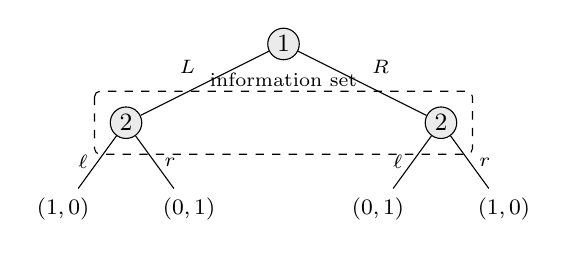
\begin{tikzpicture}[
  font=\small,
  node distance=8mm,
  inner/.style={circle, draw, fill=black!8, minimum size=4mm, inner sep=1pt},
  term/.style={rectangle, draw=none, font=\footnotesize},
  edgelbl/.style={font=\scriptsize, midway},
]
\node[inner] (p1)              {1};
\node[inner] (p2L) at (-2,-1)  {2};
\node[inner] (p2R) at ( 2,-1)  {2};
\node[term]  (o1)  at (-2.8,-2.1) {$(1,0)$};
\node[term]  (o2)  at (-1.2,-2.1) {$(0,1)$};
\node[term]  (o3)  at ( 1.2,-2.1) {$(0,1)$};
\node[term]  (o4)  at ( 2.8,-2.1) {$(1,0)$};
\draw (p1) -- node[edgelbl, above left]{$L$} (p2L);
\draw (p1) -- node[edgelbl, above right]{$R$} (p2R);
\draw (p2L) -- node[edgelbl, left]{$\ell$} (o1);
\draw (p2L) -- node[edgelbl, right]{$r$} (o2);
\draw (p2R) -- node[edgelbl, left]{$\ell$} (o3);
\draw (p2R) -- node[edgelbl, right]{$r$} (o4);
\draw[dashed, rounded corners=2pt]
  ($(p2L)+(-0.4,0.4)$) rectangle ($(p2R)+(0.4,-0.4)$);
\node[font=\scriptsize] at (0,-0.45) {information set};
\end{tikzpicture}
\end{center}

\noindent
Player~1 moves first ($L$ or $R$);  player~2 moves second but
without observing 1's choice — so 2's two decision nodes are in
one information set (the dashed box), and 2's pure strategies
are just $\{\ell, r\}$, not the four functions $\{L,R\}\to\{\ell,r\}$.

The library's EFG follows the textbook structure closely but
factors it slightly differently for the type theory:\ rather than
parameterize the tree by a player type directly, players are
factored through an \emph{information structure}:
\begin{equation}
\label{eq:infostructure}
  \InfoStruct = \bigl(\,n,\,\InfoSet : \mathrm{Fin}\,n \to \mathsf{Type},\,
                       \mathrm{arity} : \forall p\,I,\,\NN_{>0}\,\bigr),
\end{equation}
mapping each player $p \in \mathrm{Fin}\,n$ to a finite type of
information sets and each information set to a positive action
arity.  A \emph{game tree} over $\InfoStruct$ is the inductive
type
\begin{equation}
\label{eq:gametree}
\begin{aligned}
  \Tree(\InfoStruct, \Outcome) \;\coloneqq\;\;
    &\mathsf{terminal}(z : \Outcome) \\
  \mid\;& \mathsf{chance}(k, \mu : \PMF{\mathrm{Fin}\,k}, \mathrm{next} : \mathrm{Fin}\,k \to \Tree) \\
  \mid\;& \mathsf{decision}(p, I : \InfoSet_p, \mathrm{next} : \mathrm{Fin}\,(\mathrm{arity}_p\,I) \to \Tree).
\end{aligned}
\end{equation}
A decision node stores only the information-set ID; the player
identity is recovered from the structure.  An EFG is a tree paired
with a utility $\Outcome \to \Payoff{\Players}$.  Strategies come
in three flavors:
\begin{itemize}\itemsep2pt
\item \emph{Pure}: $\Spure_p = \forall I : \InfoSet_p,\, \mathrm{Fin}\,(\mathrm{arity}_p\,I)$.
\item \emph{Behavioral}: $\Sbeh_p = \forall I,\, \PMF{\mathrm{Fin}\,(\mathrm{arity}_p\,I)}$.
\item \emph{Mixed}: $\Smix_p = \PMF{\Spure_p}$.
\end{itemize}

The library's EFG semantics is \emph{distributional}:\ given a
behavioral profile $\beta : \forall p,\, \Sbeh_p$, the function
$\evalDist(\beta, t) \in \PMF{\Outcome}$ is defined by structural
recursion on $t$, with chance nodes binding the chance distribution
and decision nodes binding the player's behavioral distribution at
the relevant information set.  The compilation
$\EFG \compileTo \KG$ takes strategies to be behavioral profiles,
outcomes to be the EFG's $\Outcome$, the kernel to be $\evalDist$,
and the utility to be the EFG utility.

\designnote{Distributional, not deterministic, semantics.  An
alternative would be to evaluate to a deterministic outcome under
a pure profile and lift to mixed/behavioral profiles externally.
We chose distributional semantics because it (a) fits chance nodes
without ad-hoc lifting, (b) makes Kuhn's theorem
(\S\ref{sec:theorems:kuhn}) a purely structural identity
$\evalDist(\beta) = \evalDist(\mathrm{realize}(\mu))$ for the
realization $\mu$ of $\beta$, and (c) fits the
$\K : \prod_i \Strat_i \to \PMF{\Outcome}$ shape of \KG\ without
the strategies-to-outcomes adapter.}

An \emph{augmented} EFG in the FOSG-paper sense — a thin wrapper
over an EFG that adds a public partition over all reachable
histories and a per-player information partition over reachable
histories, including those at which the player does not act — is
also provided.  Standard EFG information sets are only defined at
decision nodes for the acting player; the augmentation lifts this
to all of history space and is the carrier on which the FOSG/EFG
bridge (\S\ref{sec:languages:bridges}) is most naturally stated.

The EFG \TT{Examples} file carries two canonical sequential games:
the 2-stage \emph{Centipede game} (Rosenthal 1981; payoffs (1,0)
/ (0,2) / (3,1) with backward-induction prediction `(p0 takes)`
leaving the welfare-max (3,1) on the table), and the
\emph{Ultimatum game} (Güth--Schmittberger--Schwarze 1982; a
proposer offers one of three splits to a responder who
accepts/rejects). Each ships with the four `evalPure` outcome
identities plus the textbook backward-induction comparison
inequalities; the full
\TT{EFGGame.IsSubgamePerfectEq} witnesses are not packaged.

\leancorr{\TT{Languages/EFG/} contains \TT{Syntax}, \TT{SOS},
\TT{Compile}, \TT{CompileObs} (compilation to ObsModelCore for
Kuhn), \TT{Augmented} (the augmented EFG), \TT{Kuhn},
\TT{Refinements} (subgame perfection,
\TT{EFGGame.IsSubgamePerfectEq}), \TT{Examples} (binary choice
plus the centipede and ultimatum), \TT{Tests}.
Supplement~§4.2.}

\subsection{Multi-agent influence diagrams}
\label{sec:languages:maid}

A \emph{multi-agent influence diagram} (MAID,
\citealp{KollerMilch2003}) represents a game as a directed acyclic
graph whose nodes are typed as one of three kinds:
\begin{itemize}\itemsep2pt
\item \emph{Chance nodes} $X$ — random variables; each carries a
  conditional probability distribution (CPD) over its domain given
  the realizations of its parents.  This is Nature's contribution.
\item \emph{Decision nodes} $D$ — each owned by a specific player;
  the parents of a decision node represent the information the
  owning player observes when deciding, and the player chooses a
  value in the node's finite domain as a function of those
  parents.
\item \emph{Utility nodes} $U$ — real-valued functions of their
  parents; each utility node is associated with a specific player,
  and that player's payoff is the sum of all their utility nodes.
\end{itemize}

\noindent
The DAG structure makes causal and informational dependence
\emph{explicit} in the syntax:\ the parent set of a decision node
is literally the information available to the deciding player, and
the parent set of a utility node is literally the variables it
depends on.  Where an EFG has to flatten the same information into
a tree with shared information sets, a MAID exposes the same
content as a Bayesian network with decision and utility annotations.

\begin{center}
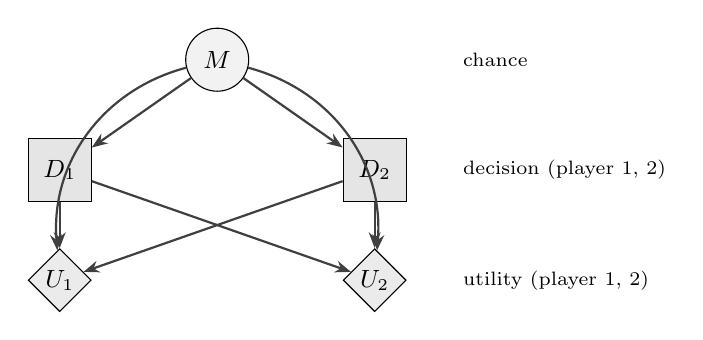
\begin{tikzpicture}[
  font=\small,
  node distance=12mm,
  chance/.style ={circle,   draw, fill=black!5,  minimum size=8mm, inner sep=1pt},
  decision/.style={rectangle,draw, fill=black!10, minimum size=8mm, inner sep=1pt},
  utility/.style ={diamond,  draw, fill=black!8,  minimum size=8mm, inner sep=1pt},
  arr/.style={-{Stealth[length=2mm]}, thick, black!75},
]
\node[chance]   (M)  at (0, 1.4)   {$M$};
\node[decision] (D1) at (-2,0)     {$D_1$};
\node[decision] (D2) at ( 2,0)     {$D_2$};
\node[utility]  (U1) at (-2,-1.4)  {$U_1$};
\node[utility]  (U2) at ( 2,-1.4)  {$U_2$};
\draw[arr] (M)  -- (D1);
\draw[arr] (M)  -- (D2);
\draw[arr] (D1) -- (U1);
\draw[arr] (D1) -- (U2);
\draw[arr] (D2) -- (U1);
\draw[arr] (D2) -- (U2);
\draw[arr] (M)  to[bend right=40] (U1);
\draw[arr] (M)  to[bend  left=40] (U2);
\node[font=\scriptsize, anchor=west] at (3.0, 1.4)   {chance};
\node[font=\scriptsize, anchor=west] at (3.0, 0)     {decision (player 1, 2)};
\node[font=\scriptsize, anchor=west] at (3.0,-1.4)   {utility (player 1, 2)};
\end{tikzpicture}
\end{center}

\noindent
A two-player MAID:\ a market state $M$ is sampled by Nature; each
player observes $M$ and chooses an action $D_i$; each player's
payoff $U_i$ depends on the market state and both decisions.
Decision nodes are squares, chance nodes are circles, utility
nodes are diamonds.

The library formalizes a finite-domain fragment:\ each node has a
finite domain, decision-node parents specify the player's
information, and utility nodes are real-valued.

The compilation $\MAID \compileTo \KG$ proceeds via an
intermediate \emph{frontier evaluator}.  At each step, the
evaluator picks a node whose parents are all assigned and either
(a) samples its chance distribution, (b) consults the player's
strategy at the appropriate information set, or (c) accumulates
its utility into the per-player running sum.  The order of
evaluation is non-trivial:\ when several decision nodes share a
parent set, the evaluator's resolution must be order-independent
to make the compilation well-defined.  The diamond/commutation
properties licensing the order-independent compiler are proved
once; the same \emph{frontier-stability} pattern reappears in the
event-graph-based protocol layer that depends on this library
\citep{KollerMilch2003}.

\tradeoff{The order-of-evaluation issue is, in our view, the
single largest design pressure in the MAID layer.  An obvious
alternative — fixing a topological order at compilation time —
would simplify the proofs but build into the formalism a choice
that no MAID-as-a-mathematical-object cares about.  We accepted
the proof obligations and got an order-independent compiler in
exchange.}

\leancorr{\TT{Languages/MAID/} contains \TT{Syntax}, \TT{SOS},
\TT{FrontierEval}, \TT{FrontierLemmas} (the diamond properties),
\TT{FoldEval}, \TT{Prefix}, \TT{Compile}, \TT{CompileObs},
\TT{Kuhn}, \TT{Theorems}.  Supplement~§4.3.}

\subsection{Multi-round games, repeated games, stochastic games}
\label{sec:languages:multiround}

A multi-round game is a finite list of
\emph{rounds}~\citep{ShohamLeytonBrown2008}, each round consisting
of a state-dependent signal distribution (nature's joint signal),
a per-player view function (state plus signal mapped to an
observation), and a deterministic state transition keyed on the
joint action profile.  Strategies are pure and memoryless at the
protocol level — a function from the player's view to an
\emph{optional} action — with mixed/behavioral and recall
structure imposed externally as analysis-layer concerns.

The library's compilation $\MR \compileTo \KG$ generates the
outcome kernel by folding the round list and threading the state
through the chain of observations and transitions.  A bounded
horizon ensures termination.  Around this layer the library also
provides two standard variants:
\begin{itemize}\itemsep2pt
\item \emph{Repeated games}:\ identical rounds with public
observation of past action profiles.  \TT{RepeatedGame.lean}
provides an infinite-horizon discounted repeated-game helper:
strategies map finite public histories to the next stage action,
payoffs are normalized discounted sums, and
\TT{constStrategy\_isDiscountedNash} records the forward direction
that a stage-game Nash action profile remains Nash under constant
repetition, assuming bounded stage payoffs.

The infinite discounted repeated-game folk theorem is not built
through the finite-list protocol syntax; it is formalized directly
on public \TT{KernelGame} profile streams in
\TT{Concepts/FolkTheorem.lean}.  In the main theorem the repeated
game is taken over the mixed extension, so period actions are
publicly observed mixed stage strategies.  In that observable
mixed-action model, every strictly individually rational feasible
payoff vector is approximated by Nash payoffs of sufficiently
patient discounted repeated games (\Cref{thm:folk-discounted}).

\item \emph{Stochastic games}~\citep{Shapley1953stochastic}:\
rounds chosen by state, with a stochastic transition.  Bounded
horizon, by design.
\end{itemize}

The multi-round layer also compiles into the generic
\emph{InfoModel}/\emph{ObsModel} substrate that the
behavioral$\,\leftrightarrow\,$mixed Kuhn theorem
(\S\ref{sec:theorems:kuhn}) is stated against.  This is the layer
at which a per-round full-recall hypothesis becomes a per-round
\emph{ActionPosteriorLocal} hypothesis sufficient for the
mixed-to-behavioral direction.

\leancorr{\TT{Languages/MultiRound/} contains \TT{Syntax},
\TT{SOS}, \TT{Compile}, \TT{CompileObs} and its linearizations
(\TT{CompileObsLin}, \TT{CompileObsLinAdequacy},
\TT{CompileObsLinRecall}), \TT{RepeatedGame}, \TT{StochasticGame},
\TT{Kuhn}, \TT{Theorems}.  Supplement~§4.4.}

\subsection{Factored-observation stochastic games}
\label{sec:languages:fosg}

To explain factored-observation stochastic games we have to
distinguish two pre-existing notions.  A \emph{stochastic
game}~\citep{Shapley1953stochastic} is a Markov game on a finite
state space:\ at each state, every active player simultaneously
chooses an action; the joint action determines a stage payoff and
a stochastic transition to a next state, and play continues to
horizon.  This formalism handles state and transition randomness
cleanly but is opaque about \emph{what each player observes}
during a transition — the textbook treatment assumes either
perfect monitoring of the state or a particular monitoring scheme
named in prose.  A \emph{factored-observation stochastic game}
(FOSG, \citealp{Kovarik2022}) makes the monitoring explicit and
\emph{factored}:\ each transition produces a per-player
\emph{private} observation (independent component per player) and
a single \emph{public} observation visible to everyone.  A player's
strategy is then a function of their own observation \emph{sequence}
— the only data the player has access to.

\begin{center}\small
\begin{tabular}{@{}lp{0.62\textwidth}@{}}
\toprule
Component & What it adds \\
\midrule
state space + transition & ``where am I, and where am I going?'' \\
active-set per state & which players must move at each state \\
per-state available actions & legality of each player's action \\
reward vector & per-step payoff to each player \\
per-player private obs & what player $i$ alone sees on a transition \\
public observation & what \emph{every} player sees on a transition \\
\bottomrule
\end{tabular}
\end{center}

\noindent
The FOSG framework subsumes the standard formalisms used in the
multi-agent reinforcement-learning literature (POMGs,
Dec-POMDPs) by an appropriate choice of private and public
observation channels, and it specializes to extensive-form games
when the per-player observation sequence is rich enough to identify
the current information set.  This is the modern carrier for
imperfect-information sequential games:\ a player's strategy can
depend only on their own observation sequence, which is
\emph{exactly} the formal counterpart of an information set in the
sequential setting.

In the library, an FOSG carries a state space, an active-set
function, per-player available actions, a transition kernel, a
reward vector, per-player private observations, and a public
observation.  Histories are recorded by an explicit history type.
The finite-horizon FOSG kernel game is the canonical native
carrier on which the bounded Kuhn theorem
(\S\ref{sec:theorems:kuhn}) is proved.

\leancorr{\TT{Languages/FOSG/} contains \TT{Basic}, \TT{History},
\TT{Information}, \TT{Strategy}, \TT{Values}, \TT{Execution},
\TT{OutcomeClosure}, \TT{Serial}, \TT{Compile}, \TT{Kuhn},
\TT{Theorems}.  Supplement~§4.5.}

\subsection{Intrinsic-form games}
\label{sec:languages:intrinsic}

A focused layer formalizes the \emph{intrinsic} (a.k.a.\
Witsenhausen-style) representation of games following
\citet{HeymannDeLaraChancelier2020}:\ rather than fixing an order
in which agents act, the syntax exposes a set of agent decision
\emph{addresses} and information sets directly.  Nature first
selects an exogenous state; choices at the addresses then have to
fit together into a global configuration.  A model is
\emph{solvable} when, for every state and every profile of local
choices, there is a unique compatible configuration and hence a
well-defined law over realized decisions.

This syntax supports the same three ways of randomizing that
appear in sequential games, but without building a tree.  A
player may draw one complete contingent plan, randomize
independently across that player's decision addresses, or randomize
independently at the information atoms the player can distinguish.  The
first comparison is unconditional:\ independent randomization by
address and behavioral randomization by information atom induce
the same local choice laws.  The second is the intrinsic analogue
of Kuhn's theorem.  If the information structure admits a causal
order and the player has perfect recall along that order, then
the conditional behavioral strategy extracted from a mixed plan
preserves the full outcome law against every opponent profile.
The conclusion is equality of distributions over realized
decision profiles, not just equality of one-address marginals.

The intrinsic layer is a separate syntactic root than
EFG/MAID/MR/FOSG, used as a target by representations that prefer
order-independent reasoning.

\leancorr{\TT{Languages/Intrinsic/} contains the strategy
carriers, causal-order and perfect-recall predicates, and the
formal outcome-law equivalence for solvable W-models.  The
definition and theorem anchors are listed in Supplement~§4.6.}

\subsection{Bridges as commuting compilations}
\label{sec:languages:bridges}

A \emph{bridge} between two languages $L_1, L_2$ is a translation
$\tau : \mathrm{Syntax}_{L_1} \to \mathrm{Syntax}_{L_2}$ paired with
a theorem stating that the two compilation paths agree under a
specified semantic relation:
\begin{equation}
\label{eq:bridge}
  R\bigl(\,L_1.\compileTo(x),\;L_2.\compileTo(\tau(x))\,\bigr).
\end{equation}
Different relations $R$ correspond to different bridge strengths:
EU-isomorphism (\S\ref{sec:semantic-core:morphisms}) is the
strongest; protocol simulation (utility-preserving but not
necessarily strategy-bijective) is intermediate;
EU-equivalence-of-equilibria is the minimum useful target.  The
library exposes the following bridges:

\begin{center}\small
\begin{tabular}{@{}llp{0.42\textwidth}@{}}
\toprule
Source & Target & Relation \\
\midrule
NFG  & EFG  & EU-isomorphism (NFG as a depth-1 EFG) \\
NFG  & FOSG & EU-isomorphism (NFG as a one-shot FOSG) \\
EFG  & NFG  & EU-equivalence on the realized strategic form \\
MAID & EFG  & strategic-form refinement (information sets preserved) \\
EFG  & FOSG & game-form simulation (FOSG view of an EFG with serial execution) \\
\bottomrule
\end{tabular}
\end{center}

The bridge theorems are stated as identities on the compiled
kernel games (or game forms), and are the glue that lets a
theorem about, say, EFG behavioral strategies be transported to a
MAID by composing the MAID$\to$EFG bridge with the relevant
strategic-form theorem on the EFG side.

\leancorr{\TT{Languages/Bridges/} contains \TT{NFG\_EFG},
\TT{NFG\_FOSG}, \TT{EFG\_NFG}, \TT{MAID\_EFG}, and \TT{FOSG/}
(\TT{ObsModelCore}, \TT{AugmentedEFG}, \TT{SerialExec}).
Supplement~§5.2.}

\subsection{Relation-parameterized expressiveness}
\label{sec:languages:expressiveness}

The library packages the bridges into a generic expressiveness
framework parameterized by a semantic relation $R$ on
$\KG$.\footnote{In the Lean code the relation, together with its
\TT{refl}/\TT{symm}/\TT{trans} proofs, is bundled in a record called
\TT{EquivalenceLens}; we mention the name only because the supplement
uses it and so does any reader who reads the source.  ``Lens'' here
is the project's bundling vocabulary; it carries no connection to
optics in functional programming or to lenses in category theory.}
A \emph{language} in this layer is a pair $(\mathrm{Syntax},
\compileTo)$ with $\compileTo$ targeting $\KG_\Players$ for some
fixed $\Players$; a \emph{reduction} $L \to M$ over a relation $R$
is a translation $\tau$ and a proof that
$R(L.\compileTo(x), M.\compileTo(\tau(x)))$ holds for every source
$x$.  Reductions compose under transitivity of $R$.

\paragraph{The relation taxonomy.}\
The library catalogues the semantic relations this framework
supports.  They form a refinement order:\ a stronger relation
determines a weaker one.

\begin{center}\small
\begin{tabular}{@{}lp{0.62\textwidth}@{}}
\toprule
Relation & What it preserves \\
\midrule
$\mathrm{ProtocolEquivalent}$ &
  Protocol isomorphism on game forms (strategies and outcomes
  relabeled bijectively, kernel preserved); ignores utility. \\
$\mathrm{UtilityDistributionEquivalent}$ &
  Bisimulation in \KG: both protocol and joint utility
  distribution preserved at every profile. \\
$\mathrm{UtilityDistributionSimulation}$ &
  One-way version of the above; the directed reduction. \\
$\mathrm{EUEquivalent}$ &
  Equal expected utility for each player at corresponding profiles
  (the equilibrium-relevant relation). \\
$\mathrm{EUSimulation}$ &
  Directed EU-comparison; equilibria of the source pull back to
  the target. \\
\bottomrule
\end{tabular}
\end{center}

\noindent
The bridges of \S\ref{sec:languages:bridges} are reductions in
this framework for the relation in their column.  Context-aware
extensions of the framework support languages whose compilation
depends on a typing/visibility context — the natural target for
downstream protocol-language formalizations.

\paragraph{Worked theorems.}\
Two concrete worked expressiveness theorems are packaged in this
form.  An expressiveness claim like ``every finite NFG is
a one-shot FOSG up to EU-isomorphism'' becomes the statement that
$\NFG \to \FOSG$ is a reduction over the EU-isomorphism relation;
``every bounded MAID is an EFG up to strategic-form refinement''
becomes the analogous reduction over the refinement relation.

\designnote{Expressiveness comparisons in the protocol-language
literature are notoriously informal.  By making the relation $R$
explicit, the library forces every comparison statement to commit
to which structural information is preserved and which is not.
The resulting lattice of bridges (NFG, EFG, MAID, MR, FOSG ordered
by which relation we can prove between them) is itself a
contribution.}

\leancorr{\TT{Languages/Expressiveness/} contains \TT{Basic}
(\TT{Language}, \TT{Reduction}), \TT{Relations} (the relation
taxonomy), \TT{CausalContext}, \TT{MAID\_EFG}, \TT{EFG\_FOSG}.
Supplement~§5.1.}

\section{A worked example end-to-end: Prisoner's Dilemma}
\label{sec:worked-example}

To anchor the abstractions of
\Crefrange{sec:semantic-core}{sec:languages}, we trace one small game
through the full syntax-to-theorem pipeline.  The example is deliberately the
smallest non-trivial one — Prisoner's Dilemma in NFG form — and
the corresponding Lean is in
\TT{Languages/NFG/Examples.lean}.

\paragraph{Source syntax.}\
The player type is $\Players = \mathrm{Bool}$, the action type is
\[
  \Act \;=\; \{\textsf{cooperate},\,\textsf{defect}\},
\]
shared between both players, and the payoff matrix is the
classical one ($r_{CC} = 2$, $r_{DD} = 1$, $r_{DC} = 3$ for the
defector and $0$ for the cooperator).  As an \TT{NFGGame}, this is
a record carrying the joint outcome type
$\prod_{i:\mathrm{Bool}} \Act$, the identity outcome map, and the
$\mathrm{Bool} \times \Act \times \Act \to \RR$ utility table.

\paragraph{Compilation to a kernel game.}\
The NFG compiler (\Cref{sec:languages:nfg}) sets the strategy type
to $\Act$ for each player, the outcome type to
$\prod_i \Act$, the kernel to the Dirac evaluation
$\Profile \mapsto \Dirac_\Profile$, and the utility to the input
table.  The resulting \TT{KernelGame} is deterministic; randomness
enters only when we lift to its mixed extension
(\Cref{sec:semantic-core:kernelgame}).

\paragraph{Solution-concept instantiation.}\
The library's $\IsNash$ predicate
(\Cref{sec:solution-concepts:nash}) on the compiled kernel game
unfolds to
\[
  \forall i : \Players,\,\forall a' \in \Act.\quad
    u_i(\Profile) \;\ge\; u_i(\Profile[i \mapsto a']),
\]
which on Prisoner's Dilemma reduces to four inequality checks per
profile.  The Lean proof
\TT{pd\_defect\_is\_nash}:\
\TT{IsNashPure prisonersDilemma pd\_defect\_defect} is a single
\TT{intro/cases/cases/simp} that discharges the four inequalities
by direct evaluation of the utility table.  The corresponding
``cooperate is not Nash'' fact is the symmetric \TT{linarith} after
unfolding the deviation to defect.

\paragraph{Mixed-strategy extension and Nash existence.}\
Lifting to the mixed extension produces a kernel game with
strategy type $\PMF{\Act}$ for each player and outcome type
$\prod_i \Act$ as before.  The library's mixed Nash existence
theorem (\Cref{thm:nash-mixed}) applies nonconstructively and
returns some mixed equilibrium of the extension.  Separately, the
worked example proves that defect is dominant, so the pure
(defect, defect) profile is Nash by the
dominance$\,\Rightarrow\,$Nash chain
(\Cref{sec:solution-concepts:dominance}) without invoking Brouwer.

\paragraph{Bridging to FOSG.}\
The NFG$\to$FOSG bridge of \Cref{sec:languages:bridges} maps
Prisoner's Dilemma to a one-shot FOSG with two world states
($\mathsf{init}, \mathsf{terminal}$), every player active at
$\mathsf{init}$, no observations, and a single deterministic
transition delivering the NFG payoff as the FOSG reward.  The
bridge theorem
\TT{NFG\_FOSG.NFGGame.toFOSG\_terminal\_iff} closes the
expressiveness contract:\ the EU of any pure profile in the FOSG
agrees with the EU in the NFG, so $\Profile^*$ remains a Nash
equilibrium under the utility-distribution-preserving morphism
transport (\Cref{thm:transport}).

\paragraph{What this trace illustrates.}\
\emph{(i)} The NFG syntax is a $\sim$30-line Lean record;
\emph{(ii)} compilation to \TT{KernelGame} is a definitional
unfolding, not a proof;
\emph{(iii)} the strategic-form theorems
(dominance$\Rightarrow$Nash; mixed existence; equilibrium
preservation under bridges) apply as black boxes once the
compilation has fixed the kernel game;
\emph{(iv)} the same game appears as a different syntactic
object in two languages (NFG and FOSG) but with definitionally
equal expected utility, so any equilibrium-level theorem proved
on one of them transports to the other.

\paragraph{Other small examples.}\
The same trace works for the other finite examples in
\TT{Languages/NFG/Examples.lean} and \TT{Languages/EFG/Examples.lean}:
each example follows the same pattern of source syntax, compilation,
and one or two solution-concept facts on the compiled game.

\section{Major theorems}
\label{sec:theorems}

The library proves the central existence and structural theorems
of finite non-cooperative game theory.  The proofs are stated on
the kernel-game/game-form layer (or on layered information-model
abstractions; see \S\ref{sec:theorems:kuhn}), and inherited by
every language via $\compileTo$.  This section sketches their
content; full proofs are in the cited Lean files.

\subsection{Existence of mixed Nash equilibria}
\label{sec:theorems:nash-mixed}

\begin{theorem}[Mixed Nash existence; \TT{KernelGame.mixed\_nash\_exists}]
\label{thm:nash-mixed}
Let $\KG$ be a kernel game with $\Players$ finite, every $\Strat_i$
finite and non-empty, and $\Outcome$ finite.  Then the mixed
extension $\KG^{\mathrm{mix}}$ admits a Nash equilibrium:\ a
profile $\Profile^* \in \prod_i \PMF{\Strat_i}$ with
\[
  \forall i,\,\forall \tau \in \PMF{\Strat_i}.\quad
    \EU(\KG^{\mathrm{mix}}, \Profile^*, i)
      \;\ge\;
    \EU(\KG^{\mathrm{mix}}, \Profile^*[i \mapsto \tau], i).
\]
\end{theorem}

\noindent\emph{Proof structure.}\ Following Nash's
original~\citep{Nash1950, Nash1951}, we define the gain map
\[
  \Phi_i(\Profile)(s)
    \;=\; \frac{\Profile_i(s) + (\mathrm{gain}_i(\Profile, s))^+}
              {1 + \sum_{s'} (\mathrm{gain}_i(\Profile, s'))^+},
  \qquad
  \mathrm{gain}_i(\Profile, s)
    \;=\;
    \EU(\KG^{\mathrm{mix}}, \Profile[i \mapsto \Dirac_s], i)
      - \EU(\KG^{\mathrm{mix}}, \Profile, i),
\]
which sends the product simplex $\prod_i \Delta(\Strat_i)$
continuously into itself.  The Brouwer fixed-point theorem from
the \TT{fixed-point-theorems-lean4}
package~\citep{harfeFixedPointTheorems} is lifted to the product
of standard simplices, and a fixed point of $\Phi$ is shown to be
a Nash equilibrium by an algebraic argument bracketing the positive
parts.

\paragraph{Why mathlib's Brouwer.}  The continuity content of the
proof — that the Nash map is continuous on a compact convex
polytope — is genuinely topological, and mechanizing the topology
of the simplex from scratch would dwarf the rest of the proof.
mathlib already provides a Brouwer-on-the-disk theorem and the
infrastructure to lift it across homeomorphisms; we use the
standard simplex's homeomorphism to a closed ball.  The product
of simplices step is handled by an explicit product-fixed-point
lemma rather than by appealing to the product theorem in topology.

\tradeoff{Brouwer is non-constructive, so mixed Nash existence is
\TT{noncomputable}.  A constructive existence proof would require
either an explicit algorithmic construction
(Lemke–Howson~\citep{LemkeHowson1964} for two-player games, or
the support-enumeration class for finite games more generally) or
a constructive fixed-point theorem on a finite simplicial
structure (Sperner's lemma~\citep{Sperner1928} suffices for
two-player games but the multi-player extension is not as clean).
We took the topological route because an existing Lean~4
mechanization of the Brouwer fixed-point theorem was available
as the standalone \TT{fixed-point-theorems-lean4}
package~\citep{harfeFixedPointTheorems}, which proves Brouwer for
nonempty compact convex subsets of finite-dimensional normed
spaces via a cubical Sperner's-lemma route (Kuhn 1960); this
gave us a ready dependency in the right shape for arbitrary $n$
players and let us focus on the strategic-form content of the
proof.  Algorithm-level Nash existence is independent enough to
live in a downstream module.}

\leancorr{Statement \TT{KernelGame.mixed\_nash\_exists} in
\TT{Theorems/NashExistenceMixed.lean}; the product-simplex
Brouwer wrapper in \TT{Concepts/ProductSimplexBrouwer.lean}.
Supplement~§6.1.}

\subsection{Existence of correlated and coarse correlated equilibria}
\label{sec:theorems:correlated-existence}

\begin{theorem}[CE / CCE existence; \TT{KernelGame.correlatedEq\_exists}, \TT{coarseCorrelatedEq\_exists}]
\label{thm:ce-exists}
Under the same finiteness hypotheses as
\Cref{thm:nash-mixed}, $\KG$ admits a correlated equilibrium and a
coarse correlated equilibrium.
\end{theorem}

\noindent\emph{Proof.}\ The independent product distribution
$\bigotimes_i \Profile^*_i$ over the mixed Nash profile
$\Profile^*$ of \Cref{thm:nash-mixed} is a correlated equilibrium
of the original $\KG$ (every recommendation-dependent deviation
factors through a constant-strategy unilateral deviation in
$\KG^{\mathrm{mix}}$).  CCE existence is the corollary
$\Pref\text{-CE}\subseteq\Pref\text{-CCE}$
(\S\ref{sec:solution-concepts:correlated}).

\tradeoff{This route gives CE existence as a corollary of
mixed Nash existence and is the cleanest path through the
finite-game machinery already in the library.  Hart and
Mas-Colell's regret-matching no-regret learning
construction~\citep{HartMasColell2000} produces CCE existence
constructively without going through Brouwer.  We have not
formalized regret-matching itself, but the existence theorem is
still available as a corollary of Nash existence; if a future
constructive Nash-existence proof becomes available the dependency
inverts trivially.}

\leancorr{\TT{KernelGame.correlatedEq\_exists} and
\TT{coarseCorrelatedEq\_exists} in
\TT{Theorems/CorrelatedEqExistence.lean}.  Supplement~§6.2.}

\subsection{The minimax theorem}
\label{sec:theorems:minimax}

\begin{theorem}[Von Neumann's minimax; \TT{KernelGame.von\_neumann\_minimax}]
\label{thm:minimax}
Let $\KG$ be a finite two-player zero-sum kernel game.  There exist
a real value $v$ and a mixed Nash profile $\sigma$ of
$\KG^{\mathrm{mix}}$ such that player $1$ cannot push player $0$'s
payoff below $v$ by deviating from $\sigma_1$, and player $0$ cannot
push their payoff above $v$ by deviating from $\sigma_0$:
\[
  \EU(\KG^{\mathrm{mix}}, \sigma, 0) = v,\qquad
  \forall s_1,\ \EU(\KG^{\mathrm{mix}}, \sigma[1 \mapsto s_1], 0) \ge v,
\]
\[
  \forall s_0,\ \EU(\KG^{\mathrm{mix}}, \sigma[0 \mapsto s_0], 0) \le v.
\]
Moreover, all mixed Nash equilibria of a two-player zero-sum game
give player $0$ the same expected utility.
\end{theorem}

\noindent\emph{Proof.}\ \Cref{thm:nash-mixed} gives existence of a
mixed Nash equilibrium.  In a two-player zero-sum game, mixed Nash
profiles give saddle-style inequalities for $\EU(\cdot, 0)$,
which combine with the zero-sum-Nash equality lemma and mixed Nash
existence to deliver the displayed guarantees.  The classical
max-min/min-max equality is the standard mathematical reading of
the finite saddle inequalities; the Lean theorem is stated in the
guarantee form above.

\leancorr{Statement \TT{KernelGame.von\_neumann\_minimax} in
\TT{Theorems/Minimax.lean}; supporting zero-sum-Nash equality in
\TT{Concepts/ZeroSumNash.lean} (\TT{IsZeroSum.nash\_eu\_eq}).
Supplement~§6.3.}

\subsection{Backward induction (Zermelo) and the one-shot deviation principle}
\label{sec:theorems:zermelo-odp}

A \emph{subgame-perfect equilibrium}~\citep{Selten1965} (SPE) of
an extensive-form game is a strategy profile that is a Nash
equilibrium not just of the whole game but of every subgame:\ the
restriction of $\sigma$ to any decision node and its descendants
is itself Nash on the subtree rooted there.  This rules out
``empty threats''  — Nash profiles that prescribe a player to do
something off-path that they would not actually want to do if the
off-path subgame were reached.  In a finite perfect-information
tree, SPE is the standard refinement of Nash equilibrium, and is
the equilibrium concept the theorems below characterize.

\begin{theorem}[One-shot deviation principle]
\label{thm:odp}
Let $G$ be a finite perfect-information extensive-form game.  A pure
profile $\sigma$ is a subgame-perfect equilibrium of $G$ iff it has
no profitable one-shot deviation:\ at every reachable decision node,
the action prescribed by $\sigma$ yields at least as much expected
utility (holding the rest of $\sigma$ fixed) as any alternative.
\end{theorem}

\begin{theorem}[Zermelo's backward induction]
\label{thm:zermelo}
Every finite perfect-information extensive-form game has a pure
subgame-perfect equilibrium.
\end{theorem}

\noindent The backward induction itself constructs, by recursion
on the tree, a profile with no profitable one-shot deviation; the
ODP closes the loop to subgame-perfection.  Two non-trivial
ingredients are worth flagging:
\begin{itemize}\itemsep2pt
\item \emph{Disjointness of subtrees in perfect-info trees}:\ in
a perfect-info tree, sibling subtrees have disjoint information-set
supports.  This is what allows backward induction to fix actions
at a decision node without breaking optimality elsewhere.

\item \emph{Reachable-decision quantification}:\ the ODP's
hypothesis quantifies over reachable decision nodes only.  An
explicit reach-by relation makes this precise and lets the proof
ignore unreachable nodes whose action choice cannot affect EU.
\end{itemize}

\tradeoff{Backward induction is constructively well-defined on a
finite tree, but the library's Zermelo is \TT{noncomputable}
because intermediate steps invoke classical reasoning to compare
real-valued utilities.  A computable variant restricting to
rational utilities would compile but is not packaged.}

\leancorr{Statements \TT{EFG.oneShotDeviation\_iff\_spe} and
\TT{EFG.zermelo} in \TT{Theorems/OneShotDeviation.lean} and
\TT{Theorems/Zermelo.lean}; the subtree disjointness lemma is
\TT{perfectInfo\_disjoint\_subtrees}; the reachability relation
is \TT{EFG.ReachBy}.  Supplement~§6.4.}

\subsection{Kuhn's theorem: \texorpdfstring{behavioral $\leftrightarrow$ mixed strategies}{behavioral vs. mixed strategies}}
\label{sec:theorems:kuhn}

Kuhn's theorem~\citep{Kuhn1953} relates two carriers of randomness
in extensive-form games:\ a \emph{mixed strategy} is a
distribution over pure strategies (a single global lottery),
while a \emph{behavioral strategy} chooses an independent local
lottery at each information set.  The two are payoff-equivalent
under recall conditions; without recall, the asymmetry is
genuine.

The library proves Kuhn's theorem on a representation-neutral
substrate, the \emph{observation model}:\ a tuple
$(\sigma, \mathrm{Obs}, \Act)$ recording the world state, each
player's observation type, and the per-observation action arity.
A behavioral profile is a per-player function
$\InfoState_i \to \PMF{\Act_i}$; a mixed profile is a per-player
distribution over the deterministic functions
$\InfoState_i \to \Act_i$.\footnote{Notational reconciliation:\
the Lean code uses \TT{runDist}/\TT{runDistPure} for the
profile-evaluation function on the observation-model carrier; we
write $\evalDist$ throughout the chapter for uniformity with the
EFG-language naming.  The two refer to the same operation
specialized to the relevant carrier.}

\begin{theorem}[Kuhn behavioral $\to$ mixed]
\label{thm:kuhn-bm}
Under the bounded-horizon hypothesis (no infinite traces) and the
\emph{no-non-trivial info-state repeat} hypothesis, every
behavioral profile $\beta$ admits an equivalent mixed profile
$\mu(\beta)$ in the sense
\[
  \evalDist(\beta) \;=\; \mu(\beta) \mathbin{\bind} \evalPure.
\]
\end{theorem}

\begin{theorem}[Kuhn mixed $\to$ behavioral]
\label{thm:kuhn-mb}
Under per-step semantic locality assumptions (sufficient for the
\emph{ActionPosteriorLocal} property), every mixed profile $\mu$
admits an equivalent behavioral profile $\beta(\mu)$ in the sense
\[
  \evalDist(\beta(\mu)) \;=\; \mu \mathbin{\bind} \evalPure.
\]
\end{theorem}

\noindent The two directions are not symmetric.  $B \to M$ does
not need recall — the mixed lottery can be constructed
ex-ante by independent product across information states — but
does need horizon-separation (which holds on snapshot-refined
$\InfoState$'s).  $M \to B$ requires the per-step recall property
that, given a player's information state, the conditional
distribution of their action under $\mu$ does not depend on
information \emph{outside} the player's recall.  This is
strictly weaker than perfect recall in the textbook sense:\ it
does not require remembering one's own past observations
literally, only that the action conditional has the right
locality.

The snapshot-refined information-state structure is packaged as a
derived layer on top of an arbitrary observation model.  A second
proof of the $M \to B$ direction is given via the mixed-Nash-induced
correlated distribution.  Language-specific Kuhn theorems for EFG,
MAID, MR, and FOSG follow by composing the language's compilation
to the observation-model layer with the generic theorem.

\tradeoff{Stating Kuhn on the observation-model layer rather than
on a specific syntactic class of EFGs is the single largest piece
of abstraction work in the library.  The benefit is that one proof
serves every language with a generic compilation through that
layer; the cost is a stack of technical infrastructure
(information-state snapshots, the locality predicates) that is not
in the textbook proof.  We judge the tradeoff to be sharply
positive:\ language-specific Kuhn theorems become single-line
corollaries of a single core result.}

\leancorr{\TT{Theorems/Kuhn/} contains \TT{ObsModel} (the
snapshot-refined wrapper), \TT{ObsModelCore}, \TT{KuhnModel}, the
two proof files \TT{BehavioralToMixedCore} and
\TT{MixedToBehavioralCore}, and \TT{CorrelatedRealization} (the
alternative $M \to B$ route).  The hypothesis predicates
\TT{NoNontrivialInfoStateRepeat}, \TT{HorizonSeparation},
\TT{ActionPosteriorLocal}, \TT{PerStepPlayerRecall} live on
\TT{ObsModelCore}.  Supplement~§6.5.}

\subsection{Welfare and welfare theorems}
\label{sec:theorems:welfare}

The library packages the basic welfare analysis:\ social welfare
is well-defined under finiteness, every
team-game welfare maximizer is Nash, and the price of stability
in a team game is $1$.  We do not formalize the deeper welfare
theorems of mechanism design here — they live in
\S\ref{sec:mechanism-auctions}.

\leancorr{\TT{Concepts/WelfareTheorems.lean}.}

\section{Mechanism design and auctions}
\label{sec:mechanism-auctions}

The mechanism-design and auction layers are direct consumers of
the kernel-game core.  They serve a dual role:\ they formalize
classical results that belong in any game-theory library, and
they smoke-test the reusability of the core.  Bayesian games and the
auction payoff layers build on the kernel-game/game-form layer and the
solution-concept catalogue; the quasilinear mechanism and
social-choice layers introduce their own finite structures (payments,
contracts, signal structures, bargaining, social-welfare functions)
while reusing the preference and solution-concept vocabulary.

\subsection{Bayesian games}
\label{sec:mech:bayesian}

A \emph{Bayesian game}~\citep{Harsanyi1967} models situations
where players have \emph{private information} that affects payoffs
— each player knows their own private state but only has a prior
belief over others'.  Harsanyi's reduction encodes this private
information as a \emph{type} $\theta_i \in \Theta_i$ for each
player; types are drawn jointly from a common-prior distribution
$\mu \in \PMF{\prod_i \Theta_i}$ known to all players, but only
$\theta_i$ is observed by player $i$.  A pure strategy is then a
contingent plan $\Theta_i \to \Act_i$ that prescribes an action
for every type the player might turn out to be.  Concretely, a
finite Bayesian game is the tuple
$(\Theta, \Act, \mu, u)$ with finite $\Theta_i, \Act_i$ and a
payoff $u : (\prod_i \Theta_i) \times (\prod_i \Act_i) \to
(\Players \to \RR)$ depending on both the realized type vector and
the chosen joint action.  Behavioral strategies replace the pure
version by
$\Theta_i \to \PMF{\Act_i}$.

The Bayesian game compiles to a kernel game via the \TT{ofEU}
adapter (\Cref{sec:semantic-core:kernelgame}), which packages an
EU-only specification as a kernel game whose point-mass outcome
carries the expected-utility payoff vector.  The strategy type is
$\Theta_i \to \Act_i$, and the outcome kernel is the deterministic
point mass at the \emph{ex-ante} expected utility
\[
  \mathrm{exAnteEU}(B, \Profile, i)
    \;=\; \sum_{\theta} \mu(\theta)\;
        u(\theta, \Profile_1(\theta_1), \dots, \Profile_n(\theta_n))(i),
\]
folded into a single payoff vector per profile.  The
type$\,\times\,$action sampling is therefore not a separate
sampling step in the kernel game's $\K$ but is folded into the EU
function — a deliberate use of \TT{ofEU} that lets every
EU-specific solution concept on \KG\ apply to Bayesian games
without further bookkeeping.

\emph{Bayesian Nash equilibrium}~\citep{Harsanyi1967} is then the
ordinary $\IsNash$ predicate of the compiled kernel game,
unfolded as
\[
  \forall i,\, \forall s' : \Theta_i \to \Act_i.\quad
    \mathrm{exAnteEU}(B, \Profile, i) \;\ge\;
    \mathrm{exAnteEU}(B, \Profile[i \mapsto s'], i).
\]
This is the ex-ante Bayes-Nash condition used by the current
library API; ex-post and interim variants are not separate packaged
definitions in this file.

\tradeoff{Continuous type spaces and continuous action spaces are
the natural setting for much of auction theory beyond
sealed-bid mechanisms with discrete bid grids.  As discussed in
\Cref{sec:prelim:pmf}, this falls outside the discrete-PMF
discipline and is not in scope.  All Bayesian-game results in the
library hold for finite type and action spaces.}

\leancorr{\TT{Mechanism/BayesianGame.lean} (\TT{BayesianGame},
\TT{exAnteEU}, \TT{toKernelGame}, \TT{BayesNash},
\TT{bayesNash\_iff\_exAnteEU}).  Supplement~§8.1.}

\subsection{Finite information design}
\label{sec:mech:info-design}

The information-design layer packages the finite Bayesian-persuasion
substrate used by signaling and disclosure examples.  A
\emph{signal structure} is a finite stochastic kernel
$S : \Omega \to \PMF{M}$ from states to public messages.  Given a
prior $\mu \in \PMF{\Omega}$, it induces the joint law
\[
  \nu_S(\omega,m) = \mu(\omega) S(m \mid \omega)
\]
over states and messages, together with the message marginal
$\nu_S^M$, whose finite-sum form is recorded as
\TT{messageMarginal\_apply}.  The predicate \TT{HasPriorMarginal}
says that a joint state-message distribution has state marginal
$\mu$; the basic theorem \TT{joint\_hasPriorMarginal} proves that
every signal structure satisfies this identity.  The library also
exposes two canonical signals:\ \TT{uninformative}, which sends the
unique message regardless of the state, and \TT{fullInformation},
which reports the realized state.

A finite persuasion problem fixes a prior, a signal structure, a
sender payoff, and a receiver payoff.  A decision rule maps public
messages to receiver actions.  Receiver optimality is written with
the unnormalized message weights
\[
  \sum_{\omega \in \Omega}
    \mu(\omega) S(m \mid \omega) u_R(\omega,a),
\]
which is equivalent to posterior expected utility whenever message
$m$ has positive probability and remains meaningful at zero-probability
messages.  A rule is \TT{IsPersuasive} when every induced action is
receiver-optimal at its message.  Sender welfare is the expected
sender utility under the induced joint distribution, with the
finite-sum form recorded as \TT{senderEU\_eq\_sum}; equivalently,
it is the sum of message-contingent sender scores
(\TT{senderEU\_eq\_sum\_senderScore}).

The signal-structure layer is intentionally a substrate rather than the
concavification (optimal-value) theorem:\ it gives the finite objects,
Bayes-plausibility invariant, persuasion predicate, and sender
objective on which finite persuasion examples and later optimal-design
theorems can be stated.

\leancorr{\TT{Mechanism/InformationDesign.lean}
(\TT{SignalStructure}, \TT{joint}, \TT{HasPriorMarginal},
\TT{joint\_hasPriorMarginal}, \TT{messageMarginal\_apply},
\TT{PersuasionProblem}, \TT{IsPersuasive},
\TT{senderEU\_eq\_sum}, \TT{senderEU\_eq\_sum\_senderScore}).}

\paragraph{Feasible posteriors and the splitting characterization.}\
A complementary, belief-based view of disclosure is packaged in
\TT{Mechanism/FeasiblePosteriors.lean}, stated fully generally with no
finiteness hypotheses.  An \emph{experiment} is a distribution
$\tau \in \PMF{\PMF{\Omega}}$ over posterior beliefs; its
\emph{mean posterior} $\overline{\tau} = \tau \mathbin{\bind}
\mathrm{id}$ averages those beliefs back to a prior.  The experiment
is \emph{Bayes-plausible} for $\mu$ exactly when
$\overline{\tau} = \mu$ — the splitting/martingale condition of
\citet{KamenicaGentzkow2011}.  Rather than route through
measure-theoretic conditioning, the file builds the canonical coupling
that realizes a Bayes-plausible experiment (the joint law
$\tau(b)\,b(\omega)$ whose belief marginal is $\tau$ and whose state
marginal is $\overline{\tau}$), proves the splitting direction
(\TT{isBayesPlausible\_iff\_coupling\_fst}), and records that the
feasible set is convex (\TT{isBayesPlausible\_bind}) and closed under
sequential composition (\TT{isBayesPlausible\_bind\_pointwise}), with
the uninformative and fully-revealing experiments as the extremes.

The multi-receiver generalization
(\TT{Mechanism/JointFeasiblePosteriors.lean}) calls a joint experiment
over profiles of posteriors \emph{feasible} when a single common-prior
coupling induces every agent's beliefs at once.  The library proves
the necessary direction — every feasible joint experiment has each
agent's marginal Bayes-plausible
(\TT{IsJointFeasible.bayesPlausible\_agentMarginal}) — and is
deliberately honest that the converse fails for two or more agents
\citep{Arieli2021}, so no full characterization is claimed.

\leancorr{\TT{Mechanism/FeasiblePosteriors.lean}
(\TT{meanPosterior}, \TT{IsBayesPlausible}, \TT{posteriorCoupling},
\TT{isBayesPlausible\_iff\_coupling\_fst},
\TT{isBayesPlausible\_bind});
\TT{Mechanism/JointFeasiblePosteriors.lean}
(\TT{IsJointFeasible},
\TT{IsJointFeasible.bayesPlausible\_agentMarginal}).}

\subsection{Mechanism design and the revelation principle}
\label{sec:mech:revelation}

A \emph{general mechanism}~\citep{Myerson1981} is a
type-space-and-action-rule
$M = (\Theta, \Act, g : ({\textstyle\prod_i}\Act_i) \to (\Players \to \RR))$;
a strategy profile is a family $(\sigma_i : \Theta_i \to \Act_i)_i$.
A \emph{direct mechanism} is a mechanism with $\Act_i = \Theta_i$;
the canonical strategy is the identity.  The Lean definition
of Bayesian incentive compatibility is the ex-ante finite condition
that truthful reporting is a Bayes-Nash equilibrium, quantified over
type-contingent misreport functions
$s'_i : \Theta_i \to \Theta_i$.

\begin{theorem}[Revelation principle]
\label{thm:revelation}
Let $M$ be a general mechanism with finite types and actions, $\mu$
a common prior over types, and $\sigma$ a Bayesian Nash equilibrium
of $M$.  Then the direct mechanism
$M^{\mathrm{direct}}$ obtained by composing each player's report with
$\sigma_i$ — i.e.\ $M^{\mathrm{direct}}(\theta) = g(\sigma(\theta))$ —
is BIC against type-contingent misreports.
\end{theorem}

\noindent The proof is the textbook argument in finite, ex-ante
form:\ a type-contingent report $s'_i$ in $M^{\mathrm{direct}}$
corresponds to the type-contingent deviation
$\theta_i \mapsto \sigma_i(s'_i(\theta_i))$ in $M$, and the Nash
hypothesis on $\sigma$ rules out profitable deviations.

\leancorr{\TT{Mechanism/MechanismDesign.lean} and
\TT{Mechanism/RevelationPrinciple.lean} (\TT{GeneralMechanism},
\TT{IsBNE}, \TT{toDirect}, \TT{revelation\_principle}).
Supplement~§8.3.}

\paragraph{Vocabulary and surrounding lemmas.}\
The library exposes \TT{isStrategyProof} as a synonym for
\TT{isIC} (the literature uses the two interchangeably).
\TT{Mechanism.socialWelfare} is the utilitarian aggregate of
per-player payoffs on a report profile, and
\TT{IsIndividuallyRational} is the participation constraint
parameterized by an outside-option function $o : \Players \to
\RR$:\ every player gets at least $o_i$ at every type profile.
The standard zero-outside-option normalization is exposed as
\TT{IsNonNegative}.  These are scaffolding for downstream
welfare-vs-truthfulness analyses.

\subsection{Dominant-strategy implementability}
\label{sec:mech:implementability}

The Bayesian mechanism above is payoff-only:\ its rule returns a
payoff vector and never names a chosen alternative.  A second
mechanism layer, \TT{SCFWithPayments}, makes the \emph{allocation}
explicit — agents have type-dependent valuations
$v_i : \Theta_i \to A \to \RR$ over a shared alternative set $A$, a
choice rule selects an alternative, and a payment rule charges each
agent — so that quasilinear utility
$v_i(\theta_i, \mathrm{choice}(\theta)) - p_i(\theta)$ is defined and
implementability acquires structural content.

\paragraph{Necessity:\ weak monotonicity.}\
A choice rule is \emph{weakly monotone} when, holding the others'
reports fixed, an agent's value gain from the alternative chosen at one
of its types over the alternative chosen at another is larger under the
first type.  Every dominant-strategy incentive-compatible mechanism has
a weakly monotone choice rule:\ adding the two truthfulness
constraints — type $\theta_i$ not wishing to report $\theta'_i$, and
$\theta'_i$ not wishing to report $\theta_i$ — cancels the payments and
leaves exactly weak monotonicity.  This is the multi-dimensional
analogue of Myerson's monotonicity~\citep{Bikhchandani2006,
Myerson1981} and the necessary half of the implementability
characterization; the converse (weak monotonicity suffices on convex
domains) is not formalized.

\paragraph{Single-parameter Myerson payments.}\
For real single-parameter direct mechanisms, the library proves the
one-dimensional implementability theorem in the envelope-payment form.
An allocation rule $x_i(\theta)$ is monotone in agent $i$'s own report
when increasing $\theta_i$ weakly increases $x_i$.  The Myerson
payment rule is
\[
  p_i(\theta)
    =
  \theta_i x_i(\theta)
    -
  \int_{0}^{\theta_i}
      x_i(z,\theta_{-i})\,dz .
\]

\begin{theorem}[Myerson payment formula and implementability]
\label{thm:myerson-payments}
Every DSIC single-parameter mechanism has a monotone allocation rule.
Conversely, every monotone allocation rule whose one-dimensional slices
are interval-integrable is implemented in dominant strategies by the
Myerson payment rule.  If the mechanism is zero-normalized and the
allocation slices are continuous, then DSIC payments are uniquely
given by the same envelope formula.
\end{theorem}

\noindent The necessity proof is the standard payment-sandwich
argument: truthfulness at reports $\theta_i$ and $b_i$ gives upper and
lower bounds on the payment difference, and their compatibility forces
monotonicity.  The sufficiency proof integrates the monotone
allocation slice and uses the envelope identity to show that every
misreport loses weakly relative to truth-telling.

\leancorr{\TT{Mechanism/Myerson.lean}
(\TT{SingleParameterMechanism}, \TT{payment\_sandwich},
\TT{isMonotone\_of\_isDSIC},
\TT{withMyersonPayment\_isDSIC\_of\_isMonotone},
\TT{payment\_eq\_myersonPayment\_of\_isDSIC\_of\_zeroNormalized}, and
\TT{existsUnique\_zeroNormalized\_payment\_of\_isMonotone}).}

\paragraph{Sufficiency:\ affine maximizers and VCG.}\
An \emph{affine maximizer} fixes positive weights $w_i$ and an
alternative bias $\kappa : A \to \RR$ and selects the alternative
maximizing $\sum_i w_i\,v_i(\theta_i, \cdot) + \kappa$, paired with
Clarke pivot payments:\ each agent is charged the externality it
imposes on the others — their best attainable weighted welfare minus
their welfare at the chosen alternative — a nonnegative transfer.
Scaling agent $i$'s utility by $w_i$ recovers the entire affine
objective at the chosen alternative — which the choice rule maximizes —
minus a charge independent of $i$'s own report, so no misreport can
help and the mechanism is dominant-strategy truthful.  By Roberts'
theorem~\citep{Roberts1979} affine maximizers are essentially the only
dominant-strategy rules on unrestricted domains; the library proves the
truthful direction, with \emph{VCG} (unit weights, no bias:\ efficient
allocation with Clarke pivot payments) as the canonical special case,
recovering the auction-layer VCG result of \Cref{sec:mech:auctions} at
the abstract level.

\leancorr{\TT{Mechanism/Monotonicity.lean}
(\TT{SCFWithPayments}, \TT{IsDSIC}, \TT{IsWeaklyMonotone},
\TT{weaklyMonotone\_of\_dsic}); \TT{Mechanism/AffineMaximizer.lean}
(\TT{affineMaximizer}, \TT{affineMaximizer\_isDSIC},
\TT{affineMaximizer\_payment\_nonneg}, \TT{vcg}, \TT{vcg\_isDSIC}).}

\subsection{K-implementation:\ influencing a game by nonnegative
transfers}
\label{sec:mech:kimplementation}

Mechanism design creates a game; \emph{k-implementation}
\citep{MondererTennenholtz2004} starts from a game that already
exists.  An interested party — unable to redesign the game, prohibit
strategies, or charge the players — observes the realized strategy
profile and commits to nonnegative transfers
$V : \prod_i X_i \to \RR_{\ge 0}^{\Players}$ on top of the players'
utilities.  Rationality is one-round dominance:\ players avoid
dominated strategies, where throughout this layer ``dominates'' means
weak dominance with a strict witness.  A transfer scheme
\emph{implements} a target set $O$ when the subsidized game has at
least one undominated profile and every undominated profile lies in
$O$; it is a \emph{$k$-implementation} when in addition the total
transfer at every surviving profile is at most $k$; the
\emph{implementation price} of $O$ is the infimum of feasible budgets.
The point of the notion is that promises off the desired path cost
nothing, so desirable outcomes are often implementable far below the
face value of the promises.  The library defines subsidies and
implementation on arbitrary kernel games — no finiteness enters the
definitions — and proves the singleton theory in a strengthened form.

\begin{theorem}[Singleton implementation price]
\label{thm:kimpl-singleton}
For a kernel game with finitely many players and finite nonempty
strategy sets, the implementation price of a singleton target
$\{z\}$ is
\[
  k(z) \;=\; \sum_{i}\; \max_{x_i \in X_i}
      \bigl( u_i(x_i, z_{-i}) - u_i(z) \bigr).
\]
The formula holds as a greatest lower bound with no further
hypotheses; the infimum is attained — and consequently $z$ is Nash iff
$\{z\}$ is 0-implementable — under the nondegeneracy condition that
every player has \emph{another} player with an alternative to its
target action.
\end{theorem}

\noindent Both refinements sharpen the original paper, which imposes
nondegeneracy on the whole statement.  An
$\varepsilon$-bump construction shows the greatest-lower-bound form is
unconditional, and a machine-checked one-player counterexample shows
where nondegeneracy is genuinely load-bearing:\ in a one-player game
with a payoff tie the target is Nash and yet no zero-budget
implementation exists, because without an opponent no strict witness
can dominate the off-target action.  Only the direction
``0-implementable $\Rightarrow$ Nash'' is hypothesis-free.  A second
subtlety justifies the finiteness:\ in infinite games a dominated
strategy need not be dominated by any \emph{undominated} strategy
(the paper's infinite-ascent example, mechanized both as an
order-theoretic core and as a concrete game), so the nonemptiness
clause of implementation can fail catastrophically.  The finite case
is repaired once and for all by a reusable maximal-element lemma for
transitive irreflexive relations on finite types.

\leancorr{\TT{Core/Subsidy.lean}; \TT{Implementation/Basic.lean}
(\TT{IsImplementation}, \TT{IsKImplementation}, \TT{implPrice});
\TT{Implementation/Singleton.lean} (\TT{implementationGap},
\TT{singletonTransfer\_isKImplementation}, \TT{implPrice\_singleton},
\TT{exists\_zero\_singletonKImplementation\_iff\_isNash});
\TT{Implementation/Examples.lean}
(\TT{onePlayerTie\_zero\_not\_mem\_implementationCosts});
\TT{Concepts/Dominance/Undominated.lean}
(\TT{InfiniteAscentCounterexample}); \TT{Math/Fintype.lean}
(\TT{exists\_maximal\_rel\_of\_finite\_trans\_irrefl}).}

\paragraph{A price calculus.}\
Because the singleton price is a closed-form functional of the
deviation gaps, structural corollaries come cheaply.  In an exact
potential game~\citep{MondererShapley1996} the gaps telescope through
the potential $\Phi$:\ the price of $\{z\}$ equals
$\sum_i \max_{x_i} (\Phi(x_i,z_{-i}) - \Phi(z))$, is bounded by
$n\,(\max \Phi - \Phi(z))$, and vanishes exactly at the local maxima
of $\Phi$ under unilateral moves — the Nash-iff-free-implementation
equivalence becomes a discrete first-order condition.  In a different
direction, if the game's outcome kernel is
$\varepsilon$-differentially private — a unilateral strategy change
multiplies every outcome probability by at most $e^{\varepsilon}$ —
and utilities lie in $[0,U]$, then every deviation gain is at most
$(e^{\varepsilon}-1)U$, so \emph{every} singleton target has price at
most $n\,(e^{\varepsilon}-1)\,U$.  This recasts the
approximate-truthfulness argument of
\citet{McSherryTalwar2007} as a uniform implementation-price bound; a
zero-utility game with a fully revealing kernel witnesses that the
converse fails.

\leancorr{\TT{Implementation/Singleton.lean}
(\TT{implPrice\_singleton\_eq\_sum\_potentialGaps},
\TT{implPrice\_singleton\_le\_card\_mul\_potentialGap},
\TT{implPrice\_singleton\_eq\_zero\_iff\_potential\_localMax});
\TT{Implementation/DifferentialPrivacy.lean}
(\TT{IsEpsilonDifferentiallyPrivate},
\TT{implPrice\_singleton\_le\_card\_mul\_dp\_bound});
\TT{Implementation/Examples.lean}
(\TT{revealingZeroUtilityGame\_not\_zeroDifferentiallyPrivate}).}

\paragraph{Mixed extensions, and a corrected Theorem 3.}\
When the interested party can observe mixed strategies themselves —
the paper's ``algorithm observability'' — transfers attach to mixed
profiles, and the paper's Theorem~3 asserts that a mixed profile is a
mixed equilibrium \emph{iff} it is 0-implementable in the mixed
extension, deriving both directions from its (unproved) regular-games
Theorem~2.  The library proves the constructive direction:\ every
observable mixed Nash profile is 0-implementable.  The converse is
\emph{false} as stated:

\begin{theorem}[Failure of the converse for unrestricted transfers]
\label{thm:kimpl-mixed-converse}
There is a two-player $2\times2$ game and a non-Nash profile $z$ of
its mixed extension together with nonnegative transfers on mixed
profiles under which the subsidized mixed extension has exactly one
undominated profile, namely $z$, at zero transfer — a
0-implementation of a non-equilibrium.
\end{theorem}

\noindent The construction rewards proximity to the target uniformly
across opponent strategies, so every non-target mix is strictly
dominated by the mix halfway closer to the target — an infinite
ascent with no maximum below the target — while a separate
off-column bonus protects the target itself and vanishes on the
desired path.  The transfer is necessarily discontinuous at the
target; the diagnosis is that the paper's Theorem~2 (and hence the
converse half of Theorem~3) requires an implicit admissibility class
for transfers.  To our knowledge this correction is new:\ the
published corrections to the paper
\citep{Eidenbenz2007, Eidenbenz2011, DengTangZheng2016} concern its
algorithmic claims only.

The \emph{corrected} converse is then proved under a semantic
admissibility hypothesis — for each player, the subsidized mixed game
must admit an \emph{undominated best response} to the target
opponents, which is exactly the selection property whose finite-game
analogue is the finite-ascent lemma.  Under it, the implementation
price of a mixed singleton equals the sum of pure-deviation gaps (the
affine-in-own-strategy structure collapses mixed deviations to a
finite maximum), the infimum is attained under the mixed
nondegeneracy condition via a distance-bump transfer whose strict
witnesses avoid the counterexample's discontinuous jump, and
zero-cost admissible implementation is equivalent to mixed Nash.  The
counterexample's transfer is proven to violate the selection
hypothesis, so the two results fit together exactly.  A concrete
\emph{analytic} sufficient condition is also formalized, resting on a
game-free compactness lemma of independent interest:\ on a compact
own-strategy space, upper-semicontinuity of every payoff column
implies that every strategy has an undominated weak dominator (Zorn's
lemma plus the finite-intersection property — no continuity in the
column variable is needed).  Consequently columnwise own
upper-semicontinuity of the subsidized payoff on the finite mixed
simplex alone implies the selection property, and the same analytic
price formula holds.  Budgets strictly above the formula are realized
by continuous positive-slack distance-penalty transfers; under the
same mixed nondegeneracy condition as above, exact attainment is by
the distance-bump transfer, whose subsidized own-payoff is a
continuous base function with a single upper-semicontinuous spike at
the target.  The regular-game interface packaging itself is also
formalized; what remains is a Theorem~2-style price statement for
arbitrary compact strategy spaces.

\leancorr{\TT{Math/Topology/WeakDominance.lean}
(\TT{exists\_pointwiseUndominated\_dominator\_of\_compact\_usc},
\TT{UpperSemicontinuous.update\_of\_le});
\TT{Implementation/Mixed.lean}
(\TT{mixedNash\_exists\_zero\_singletonKImplementation},
\TT{MixedSelectionAdmissibleAt}, \TT{mixedAdmissibleImplPrice\_singleton},
\TT{mixedSingletonDistanceTransfer},
\TT{exists\_zero\_mixedAdmissibleKImplementation\_iff\_isNash},
\TT{MixedOwnUpperSemicontinuous},
\TT{MixedOwnUpperSemicontinuous.selectionAdmissible},
\TT{mixedAnalyticImplPrice\_singleton},
\TT{mixedAnalyticImplPrice\_singleton\_of\_nondegenerate},
\TT{exists\_zero\_mixedAnalyticKImplementation\_iff\_isNash},
\TT{mixedSingletonDistanceTransfer\_analyticAdmissible},
\TT{mixedSingletonContinuousApproxTransfer});
\TT{Implementation/Regular.lean}
(\TT{RegularOwnUpperSemicontinuous},
\TT{RegularOwnUpperSemicontinuous.selectionAdmissibleAt});
\TT{Implementation/Examples.lean}
(\TT{mixedConverse\_zeroKImplementation\_and\_not\_nash},
\TT{mixedConverse\_implPrice\_singleton\_eq\_zero},
\TT{mixedConverseTransfer\_not\_selectionAdmissible}).}

\paragraph{Implementation devices and correlated equilibria.}\
Without algorithm observability the paper's Section~6 interposes a
\emph{recommendation device}:\ signals are drawn from a target
distribution $\mu$, each player privately receives its coordinate,
and transfers may depend on the signal profile and the realized
actions.  The library compiles the device and game into a kernel game
whose strategies are signal-contingent rules, relates the paper's
per-signal (interim) dominance to ex-ante dominance of the compiled
game by a law-of-total-expectation bridge, and proves the paper's
Theorems~7 and~8:\ for a correlated equilibrium $\mu$ (in particular,
for the product law of a mixed Nash profile), the obedient profile is
implemented \emph{exactly}, at zero transfer on every supported
signal, with obedience the unique undominated rule profile.
Uniqueness needs full support of $\mu$ — a rule deviating only at a
never-drawn signal is observationally obedient — and an available
non-conforming opponent action; both hypotheses are discharged on a
concrete uniform-correlated example.  The bonus that enforces
obedience is paid only when some opponent deviates, hence never on
path.

Beyond the paper, the layer distinguishes the pointwise realized
budget from the mediator's \emph{expected} outlay and proves a
quantitative generalization to arbitrary target laws:\ any device
whose obedient profile is interim dominant for $\mu$ pays in
expectation at least $\sum_i \max_{d_i}
\operatorname{swapRegret}_i(\mu,d_i)$ — so expected-zero-cost
implementation forces $\mu$ to be a correlated equilibrium — while a
regret-paying device (conditional swap-regret payments on path, the
usual bonus off path) implements every finite $\mu$ at exactly that
expected budget.  Thus the formal expected-cost device theorem has the
closed regret expression \(\sum_i \max_{d_i}
\operatorname{swapRegret}_i(\mu,d_i)\), and the zero-cost correlated
equilibrium theorem is the regret-zero case, connecting the device
layer to the regret characterization of correlated equilibria in
\Cref{sec:solution-concepts}.  Under the paper's \emph{pointwise}
budget the price is instead sandwiched between the largest one-signal
conditional regret and the largest supported sum of conditional
regrets, with equality at the lower end when regret obligations do
not overlap on the support; the general pointwise optimum is a finite
linear program, not a closed regret expression.  The linear program
itself is formalized (budget rows plus conditional-incentive rows over
on-path payments), with reusable weighted dual certificates for price
lower bounds, and a concrete overlapping instance whose exact price
$4/3$ is machine-checked to lie strictly inside the sandwich $[1,2]$.

\leancorr{\TT{Implementation/Device.lean}
(\TT{InterimDominantKImplementsDistribution},
\TT{exists\_recommendationDevice\_obedient\_zeroTransfer\_exactKImplementation},
\TT{InterimWeaklyDominates.toWeaklyDominates});
\TT{Implementation/Examples.lean}
(\TT{deviceTie\_exists\_strictRecommendationDevice\_exactKImplementation});
\TT{Implementation/Device.lean}
(expected-cost side:\ \TT{expectedRealizedTransfer},
\TT{sum\_maxSwapRegret\_le\_expectedRealizedTransfer\_of\_interimDominant},
\TT{isCorrelatedEq\_of\_interimDominantExpectedKImplDist\_zero},
\TT{regretRecommendationDevice\_obedient\_interimDominantExpectedKImplDist};
pointwise side:\ \TT{recommendationDevicePointwiseImplPrice\_sandwich},
\TT{recommendationDevicePointwiseImplPrice\_eq\_recommendationPaymentImplPrice},
\TT{le\_recommendationPaymentImplPrice\_of\_weighted\_certificate});
\TT{Implementation/DeviceLP.lean}
(\TT{recommendationPaymentFeasible\_iff\_lpFeasible},
\TT{le\_recommendationPaymentImplPrice\_of\_dual\_certificates});
\TT{Implementation/Examples.lean}
(\TT{OverlappingRegretPaymentExample.recommendationPaymentImplPrice\_strict\_between\_sandwich});
\TT{Concepts/Correlation/Regret.lean} (\TT{maxSwapRegret},
\TT{maxConditionalSwapRegret}).}

\paragraph{Signal-blind transfers, VCG, and dominance rigidity.}\
For incomplete-information (informational) games the party may see
actions but not the realized signals, so transfers are
\emph{signal-blind}.  Zero-cost implementation is then impossible in
general:\ the paper's Figure~4 game, transcribed payoff-by-payoff, has
an ex-post equilibrium that no signal-blind transfer scheme
$k$-implements for \emph{any} $k$.  The positive result (the paper's
Theorem~6) concerns VCG:\ in a combinatorial auction whose valuations
range over a quasi-field, a frugal surplus-maximizing VCG mechanism
admits a conformance bonus making the bundled truthful profile
ex-post dominant at zero cost — the library proves the underlying
Lemma~1 outright and shows by two further counterexamples that its
hypotheses are necessary (frugality, via a four-good example where a
$\Sigma$-based cheat strictly gains; bounded valuations, via a
scaling argument).  The paper's stronger claim that the truthful
profile is the \emph{unique} undominated one is governed by a general
rigidity fact:

\begin{theorem}[Dominance rigidity]
\label{thm:kimpl-rigidity}
If a strategy weakly dominates every strategy of a player, then that
player's undominated strategies are exactly those with identical
payoff against every opponent context.  Consequently, when each
coordinate of a profile weakly dominates everything, the undominated
profiles form the product of these payoff-equivalence classes, and
the target is uniquely undominated iff every class is trivial.
\end{theorem}

\noindent This turns the paper's uniqueness claim into an explicit
non-redundancy condition on the mechanism — two reports that induce
the same allocation and payments against every opponent report are
necessarily \emph{both} undominated, witnessed on a concrete
redundant-report auction — and replaces bespoke strictness
hypotheses in the device and VCG capstones by an unconditional
characterization of the undominated set.

\leancorr{\TT{Mechanism/InformationalGame.lean}
(\TT{StrategyEquivalentWithTransfer},
\TT{IsExPostDominantProfileWithTransfer.undominatedStrategyProfiles\_eq});
\TT{Implementation/Informational.lean}
(\TT{figure4\_no\_signalBlind\_kImplementation},
\TT{conformanceBonusTransfer\_isSignalBlindKImplementation\_of\_strict},
\TT{conformanceBonusTransfer\_undominatedStrategyProfiles\_eq});
\TT{Implementation/VCG.lean}
(\TT{frugal\_vcg\_bundled\_report\_ge\_qBased\_report},
\TT{conformanceBonusTransfer\_bundledTruthful\_undominatedStrategyProfiles\_eq},
\TT{lemma1\_fails\_without\_frugality\_trueUtility},
\TT{not\_exists\_uniform\_bound\_informationalGame});
\TT{Concepts/Dominance/Undominated.lean} (\TT{UtilityEquivalent},
\TT{undominatedProfiles\_eq\_utilityEquivalentClass\_of\_forall\_weaklyDominates}).}

\paragraph{The corrections literature.}\
Two of the paper's algorithmic claims were corrected later, and the
library mechanizes the corrected picture where it can be
self-contained.  The exact-implementation algorithm~OP is not
optimal~\citep{Eidenbenz2007, Eidenbenz2011}:\ on the published
counterexample the library proves \emph{both} sides — the optimal
exact cost is~$3$, and the OP-shaped transfer family has minimum
cost exactly~$5$ — so the suboptimality of the algorithm's output,
not merely of one transfer, is machine-checked.  The paper's
NP-hardness proof by a two-player SAT reduction is incorrect
\citep{Eidenbenz2007}; the corrected reductions of
\citet{DengTangZheng2016} (six players for pure dominance, two
players for dominance by mixed strategies) are the natural target for
a future \TT{SATReduction} module and are not yet formalized, as they
depend on the external constructions.

\tradeoff{Three observability regimes are deliberately distinguished:\
transfers on realized pure profiles (the base theory), transfers on
mixed profiles (Theorem~3's ``algorithm observability,'' where the
corrected converse above lives), and signal-blind transfers on
actions (devices, Figure~4, VCG).  The paper's Theorem~2 for
compact-continuous ``regular'' games is formalized in the part needed
for the mixed-extension theorem:\ the semantic selection hypothesis,
the compact upper-semicontinuity bridge that implies it, and the
regular-game interface packaging.  What is not formalized is a full
Theorem~2-style price statement for arbitrary compact strategy
spaces.  The mixed-extension counterexample above is exactly the
witness that the paper's omitted proof needs an admissibility class
for transfers; unrestricted transfers make the converse false.}

\subsection{Hidden-action contracts}
\label{sec:mech:contracts}

The principal–agent layer \TT{Mechanism/Contracts/Basic.lean}
formalizes the moral-hazard problem~\citep{Holmstrom1979}:\ a
risk-neutral agent privately chooses a costly action that
stochastically determines an outcome, and the principal designs a
payment schedule on outcomes.  The library records the agent's expected
utility (expected payment minus action cost), the principal's (expected
outcome reward minus expected payment), the welfare identity that the
two sum to social surplus
(\TT{principalUtility\_add\_agentUtility}), limited-liability and
incentive predicates, and \emph{linear contracts}
$t \mapsto \alpha\,r(t)$ with the principal-share formula
$(1-\alpha)\,\mathbb{E}[\mathrm{reward}]$
(\TT{principalUtility\_linearPayment}).  The \emph{first-best} benchmark
is the headline:\ moral hazard cannot beat the full-information surplus
(\TT{principalUtility\_le\_firstBest}).  The ``sell the firm'' contract
($\alpha = 1$) makes the agent the residual claimant, so its privately
optimal action is a surplus-maximizer
(\TT{isIncentivized\_linearPayment\_one\_iff}) — first-best
\emph{efficiency} — though the principal then extracts none of it, its
payoff falling to zero (\TT{principalUtility\_linearPayment\_one}).

\leancorr{\TT{Mechanism/Contracts/Basic.lean}
(\TT{PrincipalAgent}, \TT{agentUtility}, \TT{principalUtility},
\TT{linearPayment}, \TT{principalUtility\_add\_agentUtility},
\TT{principalUtility\_le\_firstBest}).}

\subsection{Social choice}
\label{sec:mech:social}

The library formalizes the basic social-choice setup:\ a finite
set of alternatives, a finite set of voters with strict
preferences, and a social welfare function or social choice
function, together with the structural fragments needed downstream
(preference profiles, the existence of a social-welfare-maximizing
alternative under utilitarian aggregation).  On top of this it
proves \emph{Arrow's impossibility theorem}~\citep{Arrow1951}:\
with at least three alternatives and a nonempty finite electorate,
every collectively rational social-welfare function satisfying weak
Pareto and independence of irrelevant alternatives (on the domain of
strict rankings) is dictatorial.  The proof follows Geanakoplos's
pivotal-voter argument, and a companion statement records the
dictator's strict preference as coinciding with society's on every
ranking profile.  The strategic analogue, the
Gibbard–Satterthwaite theorem~\citep{Gibbard1973, Satterthwaite1975}
— a strategy-proof social choice function with at least three
alternatives in its range and a nonempty finite electorate is
dictatorial — is also formalized, by the classical reduction to
Arrow through an induced social-welfare function.

The library also formalizes the classical results around majority
rule.  \emph{May's theorem}~\citep{May1952} characterizes the rule
axiomatically:\ over two alternatives, and for an arbitrary finite
electorate in which voters may be indifferent, a social decision
function agrees with majority rule --- the sign of the vote tally ---
on every profile if and only if it is anonymous, neutral, and
positively responsive (\TT{may\_theorem}).  \emph{Condorcet's paradox}
--- pairwise majority preference can
cycle even when every voter has a strict ranking --- is recorded as
the acyclicity failure of the majority relation
(\TT{condorcetMajority\_not\_acyclic}).  Its positive counterpart is
\emph{Black's median-voter theorem}~\citep{Black1948}:\ when
preferences are single-peaked, the median voter's ideal point is a
Condorcet winner (\TT{median\_is\_condorcet\_winner}).  \emph{Sen's
liberal paradox}~\citep{Sen1970} completes the impossibility group:\
no social decision function is simultaneously Paretian and minimally
liberal --- each of two individuals decisive over some pair of
alternatives (\TT{sen\_paretian\_liberal}).

\leancorr{\TT{Mechanism/SocialChoice.lean}, \TT{Mechanism/Arrow.lean},
\TT{Mechanism/GibbardSatterthwaite.lean}, \TT{Mechanism/Condorcet.lean},
\TT{Mechanism/MedianVoter.lean}, \TT{Mechanism/May.lean},
\TT{Mechanism/SenParetianLiberal.lean}.}

\subsection{Fair division}
\label{sec:mech:fair-division}

Fair division is organized under the mechanism/social-choice branch
because its objects are allocations and fairness predicates rather
than strategic equilibria.  The library has separate indivisible and
divisible packages.

\paragraph{Indivisible goods.}\
For finite additive valuations over indivisible goods, the library
defines envy-freeness, EF1, EFX, proportionality, and maximin-share
guarantees.  It proves the standard implications
envy-free $\Rightarrow$ EFX $\Rightarrow$ EF1 under nonnegative
valuations, and envy-free $\Rightarrow$ proportionality when all goods
are allocated.

\begin{theorem}[EF1 for indivisible goods]
\label{thm:indivisible-ef1}
For any finite set of agents and finite set of indivisible goods with
additive valuations, the envy-cycle allocation rule and the
round-robin allocation rule both return allocations that are EF1.
\end{theorem}

\begin{theorem}[Two-agent EFX]
\label{thm:indivisible-efx-two}
For two agents with additive nonnegative valuations over finitely many
indivisible goods, there exists an EFX allocation.
\end{theorem}

\begin{theorem}[MMS upper bound]
\label{thm:mms-average}
For additive nonnegative valuations, each agent's maximin share is at
most its proportional average value for the whole set of goods.
Consequently every proportional allocation is a maximin-share
allocation.
\end{theorem}

\leancorr{\TT{Mechanism/FairDivision/Indivisible/Basic.lean}
(\TT{IsEnvyFree}, \TT{IsEF1}, \TT{IsEFX},
\TT{IsEnvyFree.isProportional}, \TT{exists\_efx\_two\_agents});
\TT{Indivisible/EnvyCycle.lean}
(\TT{envyCycleAllocation\_isEF1});
\TT{Indivisible/RoundRobin.lean}
(\TT{roundRobinAllocation\_isEF1});
\TT{Indivisible/MaximinShare.lean}
(\TT{maximinShare\_le\_average}, \TT{IsProportional.isMaxminShare}).}

\paragraph{Divisible goods.}\
The divisible package treats cake-cutting on the unit interval with
finite non-atomic measure valuations.  The two-agent theorem is
cut-and-choose in the Steinhaus tradition~\citep{Steinhaus1948};
proportionality for any finite number of agents is proved by a
Dubins--Spanier-style moving-knife construction
\citep{DubinsSpanier1961}; envy-free existence for any finite number
of agents is proved through Stromquist's KKM/compactness route
\citep{Stromquist1980}.

\begin{theorem}[Divisible fair division]
\label{thm:divisible-fair-division}
Let $N$ be a nonempty finite set of agents, and let each agent have a
finite non-atomic measure on the unit interval.  Then there exists a
measurable allocation of the interval that is envy-free.  There also
exists a proportional allocation, and every envy-free allocation is
proportional under the library's finite-agent proportionality
predicate.
\end{theorem}

\leancorr{\TT{Mechanism/FairDivision/Divisible/CutAndChoose.lean}
(\TT{cutAndChoose\_ef\_exists}, \TT{cutAndChooseRule\_isEnvyFree});
\TT{Divisible/DubinsSpanier.lean}
(\TT{dubinsSpanierProportional},
\TT{dubinsSpanierRule\_isProportional});
\TT{Divisible/Stromquist.lean}
(\TT{stromquist\_envyFree\_exists});
\TT{Divisible/Existence.lean}
(\TT{proportional\_exists}, \TT{ef\_exists},
\TT{ef\_and\_proportional\_exists}).}

\subsection{Auctions}
\label{sec:mech:auctions}

The auction directory contains six formats at different
levels of completeness:

\begin{itemize}\itemsep4pt
\item \emph{Vickrey (second-price)}~\citep{Vickrey1961}.  The
highest bidder wins and pays the second-highest bid; truthful
bidding is a weakly dominant strategy.  The proof is by case
analysis on whether $i$'s valuation exceeds the maximum other bid; in
each case, the EU of bidding $v_i$ matches or exceeds the EU of
any other bid.

\item \emph{First-price sealed bid}~\citep{Vickrey1961}.  The
highest bidder pays their own bid.  The file defines the
deterministic first-price game and proves that no single bid is a
dominant strategy for any bidder.

\item \emph{All-pay auction}~\citep{KrishnaMorgan1997}.  Every
bidder pays their own bid regardless of winning.  The
formalization does not build a kernel game; it records elementary
payoff facts such as overbidding being unprofitable, winner
profit, rent dissipation, and a symmetric negative-payoff lemma.

\item \emph{Reserve Vickrey}.  A second-price auction with a reserve
price is packaged as a kernel game via the principled auction-game
interface.  The library proves dominant-strategy truthfulness and
records the usual utility identities for winners, losers, and
allocation.

\item \emph{Vickrey–Clarke–Groves (VCG)}~\citep{Vickrey1961, Clarke1971,
Groves1973}.  Generalizes Vickrey to multi-item, combinatorial
settings:\ each agent's payment equals the externality they impose
on others.  The library proves dominant-strategy incentive
compatibility for finitely many players, with the efficient
allocation supplied as a hypothesis and no finiteness imposed on the
allocation or type spaces.

\item \emph{Knapsack auctions}.  Agents have public weights and
single-parameter values; feasible binary allocations are subsets whose
total weight is at most capacity.  The welfare-maximizing allocation
rule is monotone in each agent's reported value, so the Myerson
payment rule makes the mechanism DSIC.  The same file also includes a
finite dynamic-programming optimal allocation for natural weights and
values, and a half-approximation theorem for the integral greedy rule
against the dynamic-programming optimum.
\end{itemize}

Vickrey and first-price are direct kernel-game constructions via
the \TT{ofEU} adapter.  VCG is packaged as a finite setup with an
efficient allocation rule and a payment function; all-pay is
packaged as a collection of real-valued payoff lemmas.  Solution
concepts come from \Cref{sec:solution-concepts} wherever a full
kernel game has been constructed.

\begin{theorem}[Knapsack DSIC and approximation]
\label{thm:knapsack-auction}
For a nonnegative-capacity binary knapsack auction, the
welfare-maximizing allocation rule is monotone and the mechanism using
Myerson payments is DSIC.  For natural weights and values, the dynamic
programming allocation is feasible and optimal, and the integral
greedy value is at least one half of the dynamic-programming optimum.
\end{theorem}

\tradeoff{Auctions are typically formalized in the literature
under continuous bid spaces and continuous valuations; this gives
the cleanest expressions for symmetric equilibrium bids and
expected revenue formulas.  Our discrete formalization is
faithful to the strategic content it formalizes
(truthful bidding is dominant in Vickrey/VCG; first-price has no
dominant bid; all-pay payoff inequalities are available) but is
not the primary place a researcher would go to study revenue
ranking under continuous distributions.  We treat the auction layer
primarily as a smoke test of the core library; downstream, an
extension to continuous auctions over mathlib's measure theory
would be the natural next step.}

\leancorr{\TT{Auctions/Vickrey.lean} (\TT{vickrey\_truthful\_dominant}),
\TT{Auctions/ReserveVickrey.lean}, \TT{Auctions/FirstPrice.lean},
\TT{Auctions/AllPay.lean}, \TT{Auctions/VCG.lean}, and
\TT{Auctions/Knapsack/Basic.lean}
(\TT{welfareMaximizingAllocationRule\_isMonotone},
\TT{welfareMaximizingMechanism\_isDSIC},
\TT{dynamicProgrammingOptimalAllocation\_feasible},
\TT{dynamicProgrammingOptimalAllocation\_optimal}, and
\TT{integralGreedy\_halfApprox\_dpOptimal}).  Supplement~§8.4.}

\section{The project-local Math layer}
\label{sec:math-layer}

The library has a project-local \TT{Math/} namespace between
mathlib and the game-theoretic development.  It packages
mathematical infrastructure that is needed repeatedly by the game
library but is not itself game theory.  A declaration belongs here
when it can be stated without players, utilities, equilibria,
strategies, or mechanisms.  Once those words become part of the
statement, the result belongs in \TT{GameTheory/}.

This separation keeps the kernel-game API small.  The game-theory
files can speak in terms of expected utility, mixed profiles, traces,
or information states, while the reusable algebra about PMFs,
products, couplings, finite traces, DAGs, denominator clearing, and
online regret remains available to every language layer.

\subsection{Discrete probability infrastructure}
\label{sec:math-layer:probability}

The largest part of \TT{Math/} is the discrete-probability layer.
\TT{Math.Probability} introduces the library's notation for kernels
and expected values over mathlib's \TT{PMF}.  It contains the finite
sum wrappers used throughout the paper and the bounded-tsum lemmas
that let expected utility remain meaningful on infinite outcome
carriers when utilities are bounded.  \TT{Math.ProbabilityMassFunction}
adds pushforward, bind-congruence, support, conditioning, and
monotonicity lemmas for PMFs.

Product distributions are factored into \TT{Math.PMFProduct}.  The
basic operation is \TT{pmfPi}, the independent product of finitely
many player-indexed PMFs.  The companion files record the algebra
needed by mixed extensions and information-model proofs:\ coordinate
projection, coordinate update, bind/factorization laws,
conditioning, and independence from a coordinate.  This is why the
same \TT{pmfPi} facts can support normal-form mixed extensions,
correlation regimes, observation models, MAID compilation, and
FOSG/MultiRound execution.

The probabilistic relation layer is \TT{Math.Coupling}.  It defines
relation lifting for PMFs by a joint distribution with prescribed
marginals and support contained in the relation.  This is not a game
notion, but it is the right vocabulary for bisimulation-style
arguments:\ equality of laws, projection through a view, and
one-step relational simulation are all special cases.  The companion
\TT{Math.NondeterministicRefinement} file lifts the same discipline
from single laws to families of laws indexed by an unweighted
resolution type.

\subsection{Runs, traces, and finite process closure}
\label{sec:math-layer:runs}

Several language compilers need to iterate stochastic transitions.
\TT{Math.PMFIter} provides state-only Kleisli iteration:\ starting
from a state and a transition kernel, it returns the law of the state
after a fixed number of steps.  \TT{Math.TraceRun} records the entire
finite state trace instead of only the final state.  The
parameterized version, \TT{Math.ParameterizedChain}, proves the
tower-property calculation used by Kuhn-style arguments:\ averaging
over hidden pure strategies can be represented by a single sequential
chain with local conditioning.

\TT{Math.OutcomeClosure} packages a common finite-process argument.
If a continuation value is preserved by every nonterminal step, and
the process has a rank that decreases on supported transitions, then
running the stopped process for enough fuel and projecting terminal
states recovers the initial value.  FOSG outcome closure uses this
as a game-neutral lemma; the game-specific file only supplies the
state type, terminal predicate, transition kernel, rank, and
observation map.

\subsection{Finite combinatorics and ordered structure}
\label{sec:math-layer:combinatorics}

The language layer also uses finite combinatorics that is independent
of payoffs.  \TT{Math.DAG} formalizes acyclic binary relations and
topological orders, including the equivalence between acyclicity and
existence of a topological order for finite predecessor-set DAGs.
The MAID syntax uses this to separate graph well-formedness from
strategic interpretation.  \TT{Math.BoundedLists} enumerates lists of
bounded length over a finite alphabet, a small combinatorial tool
used by finite-horizon trace and history constructions.

\TT{Math.Reindex} contains generic finite-sum and \TT{ENNReal}
tsum reindexing lemmas.  \TT{Math.SimplexApproximation} contains
the denominator-clearing estimates for finite probability vectors.
Those estimates are the arithmetic substrate for turning a feasible
mixed payoff vector into a finite periodic path in the discounted
folk-theorem development.

\TT{Math.Fintype}, \TT{Math.Fin}, and
\TT{Math/Fintype/Transport.lean} package finite-cardinality and
\TT{Fin n} transport lemmas used to move theorem statements between
arbitrary finite carrier types and canonical \TT{Fin} indices.  These
are intentionally game-free: their statements mention only functions,
subtypes, finite cardinalities, and finite sums.

\subsection{Analysis, optimization, and learning}
\label{sec:math-layer:analysis}

Some infrastructure is analytic rather than combinatorial.
\TT{Math.OptimizationLocalGlobal} states a small abstract vocabulary
for fixed points, no-improvement maps, and local optimality.  The
mixed-Nash proof uses this style to isolate the algebraic step that
turns a fixed point of the Nash map into a no-profitable-deviation
profile.

\TT{Math.OnlineLearning} is the game-free online-learning component.
Its multiplicative-weights file defines the distribution updated by
exponential weights and proves the finite-horizon external-regret
bound.  The game-theoretic self-play theorem imports that result and
then identifies each player's online losses with external-regret
gains in the kernel game.  This prevents the no-regret proof from
being entangled with equilibrium terminology.

\TT{Math.SchauderFixedPoint} proves a Schauder fixed-point theorem
for nonempty compact convex subsets of real normed spaces, using the
standalone Brouwer theorem through a finite-net approximation.  The
main mixed-Nash theorem uses the finite-dimensional Brouwer wrapper,
not Schauder.  Schauder is included because it marks the mathematical
shape of a compact-strategy extension:\ the missing layer is the
game-theoretic compactness and continuity API, not the abstract
fixed-point theorem.

\TT{Math.FixedPoint.KKM} proves the finite
Knaster--Kuratowski--Mazurkiewicz covering lemma~\citep{KKM1929} for
closed covers of the standard simplex, plus an open-cover variant.  It
is used by the Stromquist fair-division proof, but the theorem itself
is stated without agents, utilities, or cake-cutting language:

\begin{theorem}[KKM covering lemma; \TT{kkm\_closed\_cover}]
\label{thm:kkm}
Let $F_i$ be closed subsets of the standard simplex indexed by
$i : \mathrm{Fin}\,n$.  If every face of the simplex is covered by the
sets whose indices belong to that face, then all the $F_i$ have a
common point.
\end{theorem}

\TT{Math.MeasureTheory.UnitInterval} supplies the measure-theoretic
unit-interval facts consumed by divisible fair division: pushforward of
a non-atomic measure along the subtype embedding, continuity of the
cumulative distribution function, interval-measure identities, and the
existence of cuts realizing a target measure value in $[0,1]$.

\subsection{Epistemic and semantic utilities}
\label{sec:math-layer:semantic}

Finally, \TT{Math.Knowledge} records the S5 knowledge operator
induced by a view function.  It is deliberately stated without
players, priors, or payoffs:\ indistinguishability is equality of
views, knowledge is truth on the equivalence class, and coarsening is
postcomposition by a projection.  The common-knowledge files in
\TT{Concepts/Knowledge/} add the game-theoretic and probabilistic
structure on top.

The same pattern appears throughout the Math layer.  It supplies
small, reusable mathematical contracts; the game library supplies
the interpretations.  That boundary is one reason the same semantic
core can support normal-form games, extensive-form games,
information models, stochastic games, mechanisms, auctions,
cooperative games, and learning dynamics without re-proving the
underlying probability and finite-process algebra in each setting.

\leancorr{\TT{Math/Probability.lean},
\TT{Math/ProbabilityMassFunction.lean}, \TT{Math/PMFProduct/},
\TT{Math/Coupling.lean}, \TT{Math/NondeterministicRefinement.lean},
\TT{Math/PMFIter.lean}, \TT{Math/TraceRun.lean},
\TT{Math/ParameterizedChain.lean}, \TT{Math/OutcomeClosure.lean},
\TT{Math/DAG.lean}, \TT{Math/BoundedLists.lean},
\TT{Math/Reindex.lean}, \TT{Math/SimplexApproximation.lean},
\TT{Math/Fintype.lean}, \TT{Math/Fintype/Transport.lean},
\TT{Math/Fin.lean}, \TT{Math/FixedPoint/KKM.lean},
\TT{Math/MeasureTheory/UnitInterval.lean},
\TT{Math/OptimizationLocalGlobal.lean}, \TT{Math/OnlineLearning/},
\TT{Math/SchauderFixedPoint.lean}, and \TT{Math/Knowledge.lean}.}

\section{Discussion: design tradeoffs}
\label{sec:discussion}

This section collects, in one place, the design choices that
shaped the library, paired with what each gained and what each
cost.  We have referred to these tradeoffs locally throughout the
chapter; the goal here is to make the global picture explicit so
that a downstream user can decide whether the library's contract
matches their needs.

\subsection{Finite, discrete probability}
\label{sec:discussion:finite}

\paragraph{Choice.}\ Every distribution is a \TT{PMF}; every
strategy/outcome carrier is a \TT{Fintype} or carries a
\TT{Fintype} hypothesis on the relevant theorem.  No
$\sigma$-algebra is ever invoked.

\paragraph{Gained.}\ Every strategic-form definition is a
$\sum$-of-products identity that the library's \TT{simp} set can
manipulate.  No measurability hypotheses propagate through
strategy spaces, profile distributions, or outcome distributions.
Equational reasoning under the \TT{PMF} monad is mechanically
straightforward.  Compilation between languages is a calculation
on finite sums and Dirac/Bind compositions.

\paragraph{Lost.}\ The cost of mechanizing measure theory and
the catalogue of classical results that fall outside the discrete
contract are described in detail in
\S\ref{sec:prelim:pmf}; we do not repeat them here.  What §8 adds
is the consequence for downstream consumers:\ a protocol or
auction layer that builds on this library inherits the discrete
contract and must either rephrase its objects in finite/discrete
shape (e.g.\ a discretized bid grid, a finite type lattice) or
build a parallel measure-theoretic infrastructure on top of
mathlib and accept the corresponding proof obligations.  In
practice this is a hard contract:\ existing downstream users of
the library work in the discrete idiom uniformly, and the
library's design does not provide an automatic bridge to a
continuous version.  An honest reading of \S\ref{sec:prelim:pmf}
should leave the consumer with a sense of which classical
theorems they can call into and which they cannot.

\subsection{Protocol/preference split}
\label{sec:discussion:protocol-preference}

\paragraph{Choice.}\ \TT{GameForm} is utility-free; \TT{KernelGame}
adds utility.  Solution concepts exist in two forms:\ EU-specific
predicates on \TT{KernelGame} and preference-parameterized
predicates (\TT{*For}) on \TT{GameForm}.

\paragraph{Gained.}\ Theorems about strategic structure (Kuhn,
information-set machinery, the deviation hierarchy) state and
prove once at the \TT{GameForm} layer, parametric in any
preference preorder.  EU is one preference preorder; lexicographic,
maximin, or non-EU preferences are other preorders that get the
same theorems.  The library is therefore reusable for, e.g.,
ordinal-preference solution concepts without rewriting the
strategic skeleton.

\paragraph{Lost.}\ One additional indirection for \emph{generic}
users.  A user who only ever cares about expected utility writes
\TT{G.IsNash $\sigma$} and is done; a user who wants to state a
generic theorem parametric in the preference must write
\TT{G.IsNashFor pref $\sigma$} and supply the preference
explicitly.  Two versions of every solution concept exist
(\TT{IsNash}, \TT{IsNashFor}, etc.), connected by \TT{\_iff\_}
bridges; the \TT{simp} set has to know about both.  In practice the
EU-only ergonomics dominates daily use and the generic version is
visible only to library authors stating preference-parametric
theorems.

\paragraph{Why.}\ The split is motivated by classical
mechanism-design practice~\citep{Myerson1991}, where the
``social-choice rule + payment scheme = mechanism'' decomposition
is exactly the protocol/preference split made structural.  Once we
saw that several classical theorems (dominance $\Rightarrow$ Nash;
correlated $\Rightarrow$ coarse correlated; the deviation hierarchy)
were preference-agnostic, building them at the \TT{GameForm} layer
became the natural design.

\subsection{The \texttt{*For} style versus typeclass overloading}
\label{sec:discussion:for-style}

\paragraph{Choice.}\ Preferences are passed as explicit
\TT{Prop}-valued arguments to \TT{*For} solution concepts; they
are not registered as typeclass instances on \TT{KernelGame}.

\paragraph{Gained.}\ Several library theorems quantify over two
preferences at once (monotonicity of $\IsNashFor$ in the
preference; Pareto dominance, which takes a $(\Pref, \sPref)$
pair; strict-implies-weak bridges; the
transport theorems of \S\ref{sec:semantic-core:transport}, which
relate a preference either to its pullback along an outcome
bijection or to its projection through a common observed outcome
view).
With explicit-argument preferences each of these is one line; with
a typeclass-based design each would force ad-hoc local instances
and \TT{let}-binding tricks at the call site.

\paragraph{Lost.}\ Slight verbosity at the call site for the
\emph{generic} user:\ they write \TT{G.IsNashFor G.euPref}~\Profile\
instead of \TT{G.IsNash}~\Profile\ whenever they instantiate the
generic version at EU.  The EU-only user is unaffected — the
EU-specific predicates (\TT{IsNash}, \TT{IsBestResponse},
\TT{IsCorrelatedEq}, …) are exposed directly and the
\TT{\_iff\_} bridges make round-tripping free for the EU case.

\paragraph{Why.}\ The honest version of the argument is not that
typeclasses are categorically wrong here — a \TT{[Preference G]}
typeclass with a default \TT{euPref} instance would in fact make
the EU-only case ergonomically uniform.  Rather, the multi-preference
theorems listed above fit explicit-argument predicates naturally
and fit typeclasses awkwardly, and the EU-only ergonomic is
recovered cheaply by the EU-specific layer.  The library does
use a typeclass where one is the right fit:\ \TT{PrefPreorder
pref} asserts that a preference is reflexive and transitive — a
property of the relation, not a choice between relations, and
Lean's inference resolves it without diamond/multi-preference
issues.

\subsection{Solution concepts on \texttt{KernelGame} only}
\label{sec:discussion:kg-only}

\paragraph{Choice.}\ \TT{IsNash}, \TT{IsDominant}, \TT{IsBR},
\TT{IsCorrelatedEq}, etc.\ are defined on \TT{KernelGame} and on
\TT{GameForm}.  They are \emph{not} re-defined on each
representation (NFG, EFG, MAID, MultiRound, FOSG); concrete
representations bridge to the central definitions via $\toKG$.

\paragraph{Gained.}\ The library has one canonical
``\texttt{IsNash} of an EFG game'' — the \TT{IsNash} of its
compiled kernel game.  Theorems about Nash on EFGs do not have to
be re-proved each time a new EFG-like representation is added;
they are corollaries of the core theorems via composition with
$\compileTo$.  This is the workhorse of the bridge architecture
of \S\ref{sec:languages:bridges}.

\paragraph{Lost.}\ Concrete representations occasionally have a
representation-specific solution concept that is more natural in
their syntax than in the kernel-game image (subgame-perfect
equilibrium for EFGs, perfect Bayesian equilibrium for Bayesian
games).  These exist as separate definitions (e.g.\
\TT{EFG.IsSubgamePerfectEq}); the library proves their relation
to the central \TT{IsNash} as a theorem rather than building it
into the definition.

\subsection{Noncomputable definitions and classical reasoning}
\label{sec:discussion:noncomputable}

\paragraph{Choice.}\ Many definitions are \TT{noncomputable},
particularly those that invoke real-number operations, the
classical disjunction \TT{Function.update} on abstract index types,
or fixed-point theorems.  We do not attempt to expose computable
witnesses for, e.g., \TT{mixed\_nash\_exists}.

\paragraph{Gained.}\ Proofs are shorter and more uniform.  Classical
reasoning is locally invoked via \TT{open Classical in} and is
flagged at every use.  Real-number arithmetic uses mathlib's full
real-number API without restriction.

\paragraph{Lost.}\ The library is not a Nash-equilibrium algorithm.
A \TT{\#eval}-style execution will not produce a witness from
\TT{mixed\_nash\_exists}.  Constructive consumers must write their
own algorithm and prove it converges to a Nash equilibrium of the
same kernel game.

\paragraph{Why.}\ The library targets formalization of theorems,
not algorithm certification.  Brouwer's fixed-point theorem is
inherently non-constructive; replacing it with a constructive
substitute (Sperner's lemma) would change the proof shape of
\Cref{thm:nash-mixed} without changing the statement, and would
not improve the user's experience unless they happened to be
running the Lean kernel as an evaluator.  We treat constructive
existence as a separate, downstream concern.

\subsection{Distributional, not deterministic, EFG semantics}
\label{sec:discussion:efg-distributional}

\paragraph{Choice.}\ \TT{GameTree.evalDist} returns a \TT{PMF}
$\Outcome$ given a \emph{behavioral} profile.  No deterministic
``play'' function exists at the EFG level; pure strategies are
lifted to behavioral via point-mass distributions.

\paragraph{Gained.}\ Chance nodes integrate without ad-hoc
adapters.  Kuhn's theorem becomes a structural identity
$\evalDist(\beta) = (\mathrm{realize}(\mu)) \mathbin{\bind}
\evalDist^{\mathrm{pure}}$ rather than a probabilistic
equivalence, and the full game-form $\toGF$ has the
$\K : \prod_i \Strat_i \to \PMF{\Outcome}$ shape natively.

\paragraph{Lost.}\ Reasoning about a single play of an EFG (a
single deterministic execution path) requires unfolding a
\TT{PMF}.  This is a wash:\ traditional textbook reasoning quietly
assumes determinism while writing distributional formulas, so
making the distributional semantics primary forces explicit
bookkeeping in places where the textbook is implicit.

\subsection{\texorpdfstring{$\mathrm{Fin}\,n$}{Fin n} player types in bridges}
\label{sec:discussion:fin-n}

\paragraph{Choice.}\ Bridge theorems often canonicalize the
player type to $\mathrm{Fin}\,n$ for the appropriate $n$.

\paragraph{Gained.}\ A canonical concrete carrier on which to
state the bridge.  Two bridges into and out of $\mathrm{Fin}\,n$
compose without re-indexing in the middle.

\paragraph{Lost.}\ Source-game player types (e.g.\
$\mathrm{Bool}$ for two-player games) must be transported across
an equivalence \TT{Bool $\simeq$ Fin 2} to use the bridge.

\paragraph{Why.}\ \TT{KernelGame.reindex}
(\S\ref{sec:semantic-core:reindex}) makes the transport a
one-line operation.  Treating $\mathrm{Fin}\,n$ as the canonical
finite-cardinality witness lets every bridge avoid having to
pick one for itself.

\subsection{What we did not formalize and why}
\label{sec:discussion:scope}

For honesty's sake we list what is missing.

\begin{itemize}\itemsep2pt
\item \emph{Repeated and stochastic games at infinite horizon.}
The library's repeated games are bounded.  The folk-theorem-style
results (Friedman, Fudenberg–Maskin) require infinite or
discounted horizons, which interact with measure theory and
which we have not formalized.

\item \emph{Continuous strategy / type / outcome spaces.}  See
\S\ref{sec:discussion:finite}.

\item \emph{Computational complexity.}  Nash existence is
formalized; PPAD-completeness~\citep{DaskalakisGoldbergPapadimitriou2009}
is not.  Approximate-equilibrium algorithmic results are not
formalized.

\item \emph{Cooperative game theory beyond Shapley values.}  The
library defines the Shapley value and proves null-player,
additivity, linearity, and symmetry lemmas.  The full uniqueness
axiomatization, the core, the nucleolus, balanced collections, and
the Bondareva–Shapley theorem~\citep{Bondareva1963, Shapley1967}
are not formalized.

\item \emph{Impossibility theorems in social choice.}  Arrow,
Gibbard–Satterthwaite, and Sen's liberal paradox are formalizable
in this framework but are not in the current library.

\item \emph{Bayesian persuasion and information design.}
Kamenica–Gentzkow~\citep{KamenicaGentzkow2011} and successors are
out of scope.

\item \emph{Mean-field / population games.}  These require the
continuum and are out of scope.
\end{itemize}

These are not bugs; they are the boundary of the library's
contract.

\section{Related work}
\label{sec:related-work}

We organize related work along several axes:\ the textbook tradition
the library mechanizes, prior efforts to mechanize fragments of
game theory in interactive theorem provers, current Lean projects in
the same neighborhood, and adjacent formalizations in dependent type
theory or higher-order logic that could plausibly serve as alternative
platforms.

\subsection{Textbook game theory}
\label{sec:rw:textbooks}

The library's substantive content is drawn from the standard
textbook canon.  \citet{vNM1944} laid the basis for the
expected-utility decision theory the library uses without
modification; the minimax theorem first appears
in~\citet{vN1928}.  \citet{Nash1950} and~\citet{Nash1951} are the
sources for the existence theorem in the form proved in
\Cref{thm:nash-mixed}.  \citet{Aumann1974, Aumann1987} introduce
correlated equilibrium and its EU equivalence with
incentive-compatibility under a correlation device.
\citet{Selten1965} introduces subgame perfection and
\citet{Selten1975} trembling-hand perfection, both of which the
library formalizes.  The one-shot deviation principle---the
standard characterization of subgame-perfect equilibrium in
finite perfect-information games---is the form proved in
\Cref{thm:odp}.
\citet{Harsanyi1967} formalizes Bayesian games and
type-conditional strategies.  \citet{Kuhn1953} is the source of
the behavioral-vs-mixed equivalence, originally proved under
perfect recall;~\citet{Aumann1964} extended it to infinite
extensive games.
\citet{Friedman1971} and~\citet{FudenbergMaskin1986} are the
classical references for the discounted repeated-game folk theorem
formalized in \Cref{thm:folk-discounted}.

For comprehensive surveys we draw
on~\citet{OsborneRubinstein1994},
\citet{MaschlerSolanZamir2013},~\citet{ShohamLeytonBrown2008},
and~\citet{Myerson1991}.  The mechanism-design layer follows
Myerson's revelation-principle exposition;
the auction layer follows~\citet{Krishna2010}.  Algorithmic
game theory, including the price of anarchy, is treated
in~\citet{NisanRoughgardenTardosVazirani2007}, with Roughgarden's
smoothness framework~\citep{Roughgarden2015}, his selfish-routing
analysis of the price of anarchy~\citep{Roughgarden2005}, and
Koutsoupias–Papadimitriou's original
PoA~\citep{Koutsoupias1999} all relevant.

The factored-observation stochastic-game
formalism~\citep{Kovarik2022} unifies extensive-form games,
partially observable Markov games, and
multi-agent reinforcement-learning settings; the library uses it
as the most general native presentation, while keeping EFG and
NFG as distinct languages because the textbook tradition treats
them so.  The sequence-form representation
of~\citet{KollerMegiddoVonStengel1994} is conspicuously absent
from the library; we discuss this in \Cref{sec:future}.

Multi-agent influence diagrams are due
to~\citet{KollerMilch2003} and have been further developed
in~\citet{PfefferGal2007} and~\citet{HammondEtAl2023}.  The
order-independence and frontier-commutation lemmas for MAID
compilation are partly formalized in our library
(\TT{MAID/FrontierLemmas.lean}); strategic-relevance and
d-separation analyses remain extension targets.

\subsection{Prior formalizations of game theory}
\label{sec:rw:formalization}

\paragraph{Coq.}\ \citet{Vestergaard2006} gives a Coq-formalized
constructive proof of sequential Nash equilibria.
\citet{LeRouxMartinDorelSmaus2017} formalize a Nash-equilibrium
existence theorem in both Coq and Isabelle, taking a constructive
route distinct from our Brouwer-based proof.
\citet{Bertot2016} formalized the Stable Marriage / Gale–Shapley
algorithm in Coq.

\paragraph{Isabelle/HOL.}\ Lange, Caminati, Kerber, Rowat, and
collaborators have produced a substantial body of mechanized
auction theory in Isabelle, including VCG, combinatorial
auctions, and revenue-equivalence
fragments~\citep{KerberLangeRowat2016, CaminatiKerberLangeRowat2014}.
Their setting is more directly continuous than ours, since
Isabelle's analysis library makes real-valued bid spaces
ergonomic.  Isabelle's CryptHOL~\citep{Lochbihler2016} formalizes
discrete probability and probabilistic programs and has been
used for cryptographic-protocol verification rather than
game-theoretic equilibria.

\paragraph{Lean.}\ The discrete-probability monad \TT{PMF}, the
standard simplex and its convex/topological API, finite-type
infrastructure, and the surrounding analysis the library depends
on are all in mathlib~\citep{mathlib2020}; the Brouwer fixed-point
theorem itself is supplied by the standalone
\TT{fixed-point-theorems-lean4}
package~\citep{harfeFixedPointTheorems}.

The closest neighboring project is
\TT{EconCSLib}~\citep{EconCSLib2026}, a public Lean~4 library and
knowledge base for computational economics.  Its current scope
includes strategic, extensive, and coalitional games; social choice
and fair division; matching; auctions and mechanism design; and
supporting fixed-point, minimax, and linear-programming material.
The overlap with the present library is therefore substantial:
equilibrium concepts, zero-sum games, mechanism design, voting,
auctions, matching, and cooperative-game primitives all appear in
both developments.

The projects nevertheless have different design centers.
\TT{EconCSLib} is organized as a broad computational-economics
library, with lightweight domain-specific APIs, locally stated
assumptions, and a large blueprint/knowledge-base layer.  The
present library is organized around semantic interoperability:
\TT{GameForm} and \TT{KernelGame} are the common stochastic targets,
and the language layer proves compilation and bridge theorems from
NFG, EFG, MAID, FOSG, multi-round, and intrinsic presentations into
that target.  The two code bases are not API-compatible, but the
mathematical overlap is large enough that a shared
crosswalk of definitions, theorem statements, and intended adapters
would be valuable.  Such coordination would reduce duplicated proof
engineering and clarify which results should be shared, ported, or
kept deliberately separate because they serve different interfaces.

Several Lean developments focus on the Nash-existence slice.
\TT{math-xmum/Brouwer}~\citep{MathXMUMBrouwer2026} and the
\TT{Solo-ary/Game-Theory-Formalization}
artifact~\citep{SoloAryGameTheoryFormalization2026} both formalize
a Scarf/Brouwer route to mixed Nash equilibria in finite games.
These are directly relevant to our \Cref{thm:nash-mixed} proof
route, but their stated endpoint is narrower:\ fixed-point
infrastructure and Nash existence, not a multi-language semantic
library with theorem transport across representations.
\TT{MixedMatched/formalizing-game-theory}
~\citep{MixedMatchedFormalizingGameTheory} is an exploratory Lean
formalization of game-theoretic structures, including heterogeneous
strategy types and pure/mixed strategy profiles.  It is useful as a
modeling comparison, but it does not try to provide the language
layer, representation bridges, or theorem suite developed here.

Other Lean projects overlap with specific subfields rather than with
the whole library.  \TT{lean-social-choice}
~\citep{LeanSocialChoice} formalizes social-choice results including
Arrow's theorem; \TT{apportionmentlib}~\citep{Apportionmentlib2026}
formalizes apportionment theory, including Balinski--Young-style
impossibility results.  The combinatorial-games library
\citep{LeanCombinatorialGames} develops Conway-style terminating
two-player perfect-information games, nimbers, and surreal-number
connections.  It is deep game theory, but it is a different
formalism from the stochastic, expected-utility, partial-information
games treated here.

Among the Lean projects we found, the feature combination emphasized
in this paper remains distinctive:\ a protocol/preference split, a
multi-language layer, FOSG and MAID/EFG bridges, the Kuhn theorem at
an observation-model level, and mechanism-design constructions all
inside one semantic framework.  This is the comparison that matters
for the claims made here; it is not a claim that other Lean
formalizations are merely isolated or that future coordination is
unnecessary.

\paragraph{Other systems.}\ ACL2, HOL4, and Mizar each have
isolated game-theoretic results we are aware of but no substantial
library; we omit them for space.

\subsection{Verified probability and probabilistic programming}
\label{sec:rw:probability}

The library's reliance on \TT{PMF} places it in a tradition of
discrete probability formalizations.  \citet{HurdMcIverMorgan2005}
mechanized probabilistic guarded commands in HOL, and
\citet{Audebaud2009} formalized proofs of randomized algorithms
in Coq, both with semantic foundations that anticipate the
discrete Giry monad.  \citet{Tassarotti2019} developed a
separation logic for concurrent randomized programs in Coq.
\citet{Lochbihler2016} (CryptHOL) does similar
work in Isabelle, with cryptographic applications.  Mathlib's
\TT{PMF}~\citep{mathlib2020} provides the API on which our
library builds.

The measure-theoretic side is more developed in mathlib than the
discrete side, with substantial integration across the Lean Borel,
Lebesgue, and product-measure infrastructures; an extension of the
present library over mathlib's measure theory would draw on this.

\subsection{Mechanized programming-language semantics}
\label{sec:rw:pl}

The library's language layer borrows several patterns from
mechanized programming-language semantics:\ structural
operational semantics, denotational compilation into a common
target, simulation/refinement~\citep{Milner1989, AbramskyJung1994,
HarperPLFA, BentonHurKennedyMcBride2014}, and CompCert-style
verified-translation pipelines~\citep{Leroy2009}.  The
``language as syntax + compiler to a common semantics'' framing
is direct PL practice; what is unusual in our setting is that the
common semantics is a strategic object (a kernel game) rather
than a behavioral one.

\subsection{Categorical game theory}
\label{sec:rw:category}

A growing body of work treats games and strategies as objects in
a category with a compositional algebra of game forms.
\citet{Pavlovic2009, Hyland2010} are early examples;
\citet{GhaniHedgesWinschelZahn2018} introduce \emph{open games}
and the bidirectional ``selection function'' approach;
\citet{Joyal1977} pioneered the categorical view of two-player
games (in a logical setting).  Our protocol-map and simulation
infrastructure is inspired by this tradition without committing
to any of its specific frameworks.  An open-games-as-coalgebras
approach would be a natural reformulation; we did not take it
because the kernel-game record is already small enough that
adding a categorical superstructure would, on net, cost
ergonomics.

\subsection{Mechanized formal verification of equilibria in protocols}
\label{sec:rw:protocols}

A different line of work mechanizes
equilibrium reasoning about cryptographic and economic protocols
directly.  \citet{HalpernPass2008, AbrahamDolevGonenHalpern2006}
and successors formalize rationality-based protocol analysis and
incentive-compatible distributed algorithms.

Recent Lean case studies are in the same spirit.  The
\TT{VerifiedHandshake} artifact~\citep{VerifiedHandshake2026}
mechanizes a commitment wrapper for Stag-Hunt-ordered games and
audits the axiom footprint of the proved statements.  It is not a
general game-theory library; it is a sharp example of a
protocol-specific equilibrium theorem.  Lean AMM work is similarly
specific:\ \citet{PuscedduBartoletti2024AMM} and the associated
\TT{lean4-amm} repository~\citep{Lean4AMM} formalize automated
market-maker state and economic properties, while
\TT{amm-axioms-lean}~\citep{AMMAxiomsLean2026} derives
constant-product and weighted-geometric-mean AMM behavior from swap
axioms.  These projects should be viewed as downstream or adjacent
economic-protocol formalizations, not as substitutes for a reusable
library of game representations.  They typically commit to one
domain model and prove protocol-specific results.  Our library is
meant to make that style of work less bespoke by supplying the
strategic-form infrastructure, equilibrium predicates, stochastic
semantics, and representation bridges that such developments would
otherwise build by hand.

\section{Future directions}
\label{sec:future}

The library is intentionally a foundation:\ it is meant to be
extended.  We list the extensions we view as natural, in
descending order of how much existing infrastructure they would
re-use.

\subsection{Algorithmic and constructive Nash}
\label{sec:future:algo}

\Cref{thm:nash-mixed} is non-constructive (Brouwer); a natural
extension is a constructive proof for two-player games via the
\emph{Lemke–Howson} pivoting algorithm~\citep{LemkeHowson1964} or
via \emph{Sperner's lemma}~\citep{Sperner1928} (a combinatorial
fixed-point statement on triangulated simplices that yields
Brouwer constructively for low dimensions), packaged as an
algorithmic witness function on top of the existing strategic-form
definitions.  The \emph{PPAD}-hardness
story~\citep{DaskalakisGoldbergPapadimitriou2009} — where PPAD is
the complexity class of problems whose existence is guaranteed by
a parity argument on a directed graph, the canonical example being
end-of-line — is at a different level (it concerns problem
reductions, not proof-of-existence) and is largely orthogonal:\ a
complexity formalization would need an independent computation
model.

\subsection{Sequence form and efficient EFG solving}
\label{sec:future:sequence-form}

A \emph{sequence} in an extensive-form game with perfect recall is
the list of own-actions a player has taken along a history.  The
\emph{sequence-form representation}
of~\citet{KollerMegiddoVonStengel1994} (see also the survey
of~\citet{vonStengel2002}) replaces the exponential-sized pure
strategy space by realization probabilities indexed by sequences,
turning equilibrium computation into a linear or quadratic
program of size polynomial in the tree.  Adding the sequence-form bridge as a fourth EFG
strategy carrier (alongside pure, behavioral, mixed) would let
the library state and prove correctness of the standard solving
algorithms (LP duality$\Rightarrow$two-player zero-sum value;
sequence-form quadratic program for general-sum games).  The
Kuhn-theorem infrastructure of \Cref{sec:theorems:kuhn} already
supplies the recall layer.

\subsection{Counterfactual regret minimization}
\label{sec:future:cfr}

\emph{Counterfactual regret minimization} (CFR,
\citealp{Zinkevich2007CFR}) is the dominant family of algorithms
for finding approximate equilibria in large imperfect-information
extensive-form games; it works by tracking, at each information
set, the cumulative regret for not having played each action,
counterfactually weighted by the probability of reaching that
information set under the opponents' play.  The regret-equilibrium
duality and the no-regret learning machinery a CFR proof would
consume are already formalized (\Cref{sec:solution-concepts:regret},
\Cref{sec:theorems:learning}) — including explicit routes to
$\varepsilon$-CCE via no-regret self-play without going through
Brouwer at each finite horizon.  What remains specific to CFR is the counterfactual,
information-set-local regret decomposition for extensive-form games
and its convergence proof on top of that base.

\subsection{Imperfect-recall extensions}
\label{sec:future:absent-mind}

The Kuhn theorem in the library handles a recall hypothesis
weaker than perfect recall (per-step ActionPosteriorLocal).  The
basic \emph{absent-minded-driver}
phenomenon~\citep{PiccioneRubinstein1997} is formalized in
\TT{Languages/MultiRound/AbsentMindedDriver.lean}.  The protocol
has one player and two indistinguishable decision rounds; it
violates \TT{ViewDeterminesRound}, the MultiRound
no-absent-mindedness condition.  The payoff calculation is also
mechanized:\ with payoffs $0$ for the first exit, $4$ for the
second exit, and $1$ for missing both exits, the ex-ante optimal
continuation probability is $2/3$, while decision-time
re-optimization at the single information set under those arrival
odds chooses $1/3$ and strictly improves the decision-time value.

Natural extensions are the broader imperfect-recall pathologies
around this example:\ general conditions for time consistency,
relations between information-set revisitation and behavioral
optimality, and representation-neutral EFG/FOSG versions of the
same construction.  These should live on the observation-model
layer already used by Kuhn's theorem, with the MultiRound example
serving as the finite sanity check.

\subsection{Infinite and continuous games}
\label{sec:future:infinite}

The largest single extension would be to relax the discrete-PMF
discipline and use mathlib's measure theory.  This would let the
library state and prove:\ Glicksberg's theorem on continuous
payoff functions over compact strategy
spaces~\citep{Glicksberg1952}, the Milgrom–Weber existence theorem
for Bayesian games with uncountable type
spaces~\citep{MilgromWeber1985}, infinite-horizon discounted
stochastic games~\citep{Shapley1953stochastic, MertensNeyman1981},
and continuous-action or public-randomization variants of the folk
theorem.  The current library proves the discrete observable
mixed-action approximate discounted folk theorem of
\Cref{thm:folk-discounted}; a measure-theoretic extension would
give it continuous companions.

This is a substantial extension and would change the library's
character.  The fixed-point ingredient is partly isolated:
\TT{Math/SchauderFixedPoint.lean} proves Schauder's theorem for
compact convex subsets of real normed spaces.  What remains for
continuous games is not just a fixed-point theorem but the
measure-theoretic and topological game layer around it.  We see
that less as a single project and more as a parallel library with
shared infrastructure (the
\TT{KernelGame}/\TT{GameForm} skeleton generalizes to a kernel
$\K : \prod_i \Strat_i \to \mathcal{P}(\Outcome)$ for a measure
type $\mathcal{P}$, with the discrete \TT{PMF} as one
instantiation).

\subsection{Cooperative game theory}
\label{sec:future:cooperative}

The cooperative branch lives at \TT{Cooperative/} (a parallel
paradigm to the non-cooperative core occupying the rest of the
library; see \Cref{sec:theorems:shapley-uniqueness} for the
framing).  Already formalized:\ TU coalitional games with the
Shapley value~\citep{Shapley1953} and the four classical axioms
used by the Lean uniqueness theorem,
the unanimity-basis decomposition (Möbius inversion on the subset
lattice), the full Shapley uniqueness theorem
(\Cref{thm:shapley-unique}), the Banzhaf~\citep{Banzhaf1965} and
Shapley–Shubik~\citep{ShapleyShubik1954} power indices, simple
(voting) games, convex (supermodular) games with the
$\mathrm{IsConvex} \Leftrightarrow$ monotone-marginals characterization
\citep{Shapley1971} and closure under sum and nonnegative scalar,
the core (efficient $\land$ coalition-rational) with the
convex-set closure property and individual rationality, core
closure under finite sums and nonnegative scalar multiplication,
the Shapley-in-core theorem for convex games (hence nonempty core),
the positive-cone specialization through nonnegative
unanimity-basis coefficients, additive games (the identity
allocation), and the 3-player majority game as a worked example.
The \emph{cost of stability}~\citep{Bachrach2009} — the least external
subsidy that makes the grand coalition stable — is formalized
(\TT{IsStabilizable}, \TT{costOfStability}) with its monotonicity, the
vanishing of the cost on games with a nonempty core, and zero-cost
classes (nonnegative unanimity coefficients, additive games).
Balanced collections and the easy direction of the
\emph{Bondareva–Shapley} theorem~\citep{Bondareva1963, Shapley1967}
— a nonempty core implies balancedness — are formalized
(\TT{IsBalancedCollection}, \TT{CoalGame.IsBalanced},
\TT{IsCore.isBalanced}) by the double-counting swap over a core
allocation.
Nash bargaining
\citep{Nash1950bargaining} is formalized through the IR / weak-Pareto
characterization (the Nash maximizer is only weakly Pareto on the
disagreement boundary in this general non-convex setting), with
symmetric and affine-invariant variants;
the \emph{egalitarian} bargaining solution~\citep{Kalai1977} is also
formalized as \TT{IsEgalitarian} (the maximal feasible equal-gain
point), together with the fact that it gives at least the common gain
of the symmetric Nash solution, and the
\emph{Kalai–Smorodinsky} solution~\citep{KalaiSmorodinsky1975} through
its proportionality characterization
(\TT{IsKalaiSmorodinskyRelativeTo}, carrying IR, strong Pareto,
symmetry, and affine invariance for any reference point), with the
solution proper (\TT{IsKalaiSmorodinsky}) fixing the ideal point and
bounding each player's gain by it.
Stable matching~\citep{GaleShapley1962} is formalized through the
\TT{IsMatching}/\TT{IsBlockingPair}/\TT{IsStable} predicates, with the
existence of a stable matching proved via the Gale–Shapley
deferred-acceptance algorithm (\Cref{thm:gale-shapley}).

Natural extensions:\ the converse (hard) direction of
Bondareva–Shapley \citep{Bondareva1963, Shapley1967} — balancedness
implies a nonempty core — which closes the characterization of
core-nonempty games and is the flagship LP-duality (Farkas) result;
the nucleolus \citep{Schmeidler1969}; the Aumann–Shapley value for non-atomic
games~\citep{AumannShapley1974}; NTU coalitional games; and further
bargaining solutions.

\subsection{Information design and signaling}
\label{sec:future:info-design}

In \emph{Bayesian persuasion}~\citep{KamenicaGentzkow2011} a
sender designs an information structure (a signal-generation
mechanism that maps the state of the world to a public message)
to influence a receiver's posterior beliefs and hence their
action; the design problem is to choose the most persuasive
signal mechanism subject to the receiver's Bayesian rationality.
\emph{Signaling games}~\citep{Spence1973} are the strategic
analogue with an informed sender choosing a costly signal whose
cost may itself depend on type.  \emph{Information
design}~\citep{Bergemann2019} generalizes the persuasion setup to
multiple receivers and richer outcome rules.

The finite substrate is formalized in
\TT{Mechanism/InformationDesign.lean}:\ finite signal structures
$\Omega \to \PMF{M}$, induced joint state-message laws, the
message marginal formula, the Bayes-plausibility invariant,
uninformative and full-information signals, finite sender/receiver
persuasion problems, persuasive decision rules, and finite-sum
expressions for sender expected utility.  This is the right layer
for discrete persuasion examples and for connecting disclosure
problems back to the Bayesian-game infrastructure of
\Cref{sec:mech:bayesian}.  A complementary belief-based layer
(\Cref{sec:mech:info-design}) provides the Bayes-plausibility
\emph{splitting} characterization via the canonical posterior coupling
and its multi-receiver necessary direction~\citep{Arieli2021}.

Natural extensions are substantive theorems over this substrate:
finite concavification of the optimal sender value, value-of-information
results, optimal signal existence on a bounded finite message alphabet,
explicit finite signaling-game refinements, positive characterizations
or counterexample libraries for multi-receiver feasibility, and bridges
from persuasive decision rules to direct mechanisms.  Continuous type spaces and compact belief simplices
would require the measure-theoretic extension discussed in
\Cref{sec:future:infinite}; the finite layer is useful independently
and should remain separate from that analytic generalization.

\subsection{Social choice impossibility theorems}
\label{sec:future:social-choice}

\emph{Arrow's impossibility theorem}~\citep{Arrow1951} — no
social-welfare function aggregating individual ordinal preferences
over $\ge 3$ alternatives can simultaneously satisfy unanimity,
non-dictatorship, and independence of irrelevant alternatives — is
formalized (\Cref{sec:mech:social}, \TT{Mechanism/Arrow.lean}),
via Geanakoplos's pivotal-voter argument on a strict-linear-order
rationality layer.  Its strategic analogue
\emph{Gibbard–Satterthwaite} \citep{Gibbard1973, Satterthwaite1975}
— any non-dictatorial social choice function with full range over
$\ge 3$ alternatives is manipulable — is formalized as well
(\TT{Mechanism/GibbardSatterthwaite.lean}), by the reduction to
Arrow through an induced social-welfare function.
\emph{Sen's liberal paradox}~\citep{Sen1970}, showing that even a
minimal individual-rights condition is inconsistent with Pareto
efficiency plus universal domain, is formalized as well
(\Cref{sec:mech:social}, \TT{Mechanism/SenParetianLiberal.lean}), on
the same strict-ranking social-choice layer.  With the ordinal
impossibility results in place, the natural extensions are the
randomized and quantitative refinements — probabilistic social choice
and manipulation-robustness bounds — that would build on the library's
discrete-probability layer.

\subsection{Multi-agent learning}
\label{sec:future:learning}

With the no-regret core in place (\Cref{sec:theorems:learning}), the
open directions are the asymptotic and internal-regret refinements.
The multiplicative-weights and self-play bounds are stated for a
\emph{fixed} learning rate, where the residual error does not
vanish; the horizon-dependent tuning $\eta \approx \sqrt{\log|A|/T}$
that makes external regret sublinear — and so turns the per-horizon
$\varepsilon$-bound into a genuine \emph{convergence} statement — is
the natural next step \citep{Cesa-BianchiLugosi2006,
BlumMansour2007}.  Beyond it:\ internal-regret minimization driving
play to \emph{correlated} (not merely coarse correlated)
equilibrium; Robinson's theorem that fictitious play converges in
two-player zero-sum games; and the reinforcement-learning algorithms
(self-play with function approximation, MCTS) that the FOSG and
observation-model layers were built to host.

\subsection{Stable matching beyond existence}
\label{sec:future:matching}

The Gale–Shapley deferred-acceptance algorithm and the existence of a
stable matching from an arbitrary strict preference
profile~\citep{GaleShapley1962} are formalized
(\Cref{thm:gale-shapley}, \TT{Cooperative/GaleShapley.lean}), together
with proposer-optimality and receiver-pessimality
(\TT{daMatching\_man\_optimal}, \TT{daMatching\_woman\_pessimal}).  The
natural extensions are the remaining structural results:\ the lattice
structure of the set of stable matchings, strategy-proofness for the
proposing side, and the many-to-one (hospitals/residents)
generalization with the rural-hospitals theorem.  A computable
extraction of the $O(n^2)$ algorithm paired with the existing
correctness proof is a further refinement; Bertot's Coq
formalization \citep{Bertot2016} is a useful reference point.

\subsection{Type-theoretic refactoring opportunities}
\label{sec:future:refactor}

We close with two design directions internal to the library
itself.  First, an open-games-style
reformulation~\citep{GhaniHedgesWinschelZahn2018} would expose the
\TT{KernelGame} category in a shape suitable for compositional
reasoning at a higher abstraction level; this would not change
the theorems but might simplify their proofs.  Second, the
library's \TT{noncomputable} discipline could be tightened by
isolating the constructive fragment (definitions and theorems
that do not invoke classical reasoning) as a separately-named
namespace; this would make the boundary between the constructive
finite-game fragment and the non-constructive existence-of-Nash
fragment visible in user code.


\bibliographystyle{plainnat}
\bibliography{references}

\end{document}
